\documentclass[twoside]{NSF}
 \usepackage{xcolor}
 \usepackage{amssymb}
\usepackage{rotate}
\let\oldemptyset\emptyset
\let\emptyset\varnothing
\usepackage{pifont}
\usepackage{array}

\newcolumntype{R}[1]{>{\raggedright\arraybackslash}p{#1}}
\useunder{\uline}{\ul}{}

\usepackage{ textcomp }
\usepackage[para,online,flushleft]{threeparttable}

\def\changemargin#1#2{\list{}{\rightmargin#2\leftmargin#1}\item[]}
\let\endchangemargin=\endlist 
\usepackage{makecell}
  \usepackage[T1]{fontenc} 
    \usepackage{textcomp} 
   \usepackage{mathpazo} 
   \usepackage{framed}
      \usepackage{pifont}
\usepackage{adjustbox}
\usepackage{epstopdf}
\epstopdfDeclareGraphicsRule{.gif}{png}{.png}{convert gif:#1 png:\OutputFile}
\AppendGraphicsExtensions{.gif}
\usepackage{rotating}
\usepackage{framed}
\usepackage{colortbl}
\usepackage{wrapfig}
\usepackage{color, soul}
\sethlcolor{red}
\makeatletter
\def\SOUL@hlpreamble{%
    \setul{\dp\strutbox}{\dimexpr\ht\strutbox+\dp\strutbox\relax}%
    \let\SOUL@stcolor\SOUL@hlcolor
    \SOUL@stpreamble
}
\makeatother

% \usepackage{draftwatermark}
% \SetWatermarkText{Draft}
% \SetWatermarkScale{1}
% \SetWatermarkLightness{.91}

\usepackage{pgfplots}
  
\definecolor{maroon}{cmyk}{0,0.87,0.68,0.32}
\setlength{\parskip}{0.5mm}
\usepackage{indentfirst}
\setlength{\parindent}{0.75cm}

\usepackage{tcolorbox}

\newcommand{\quart}[4]{\begin{picture}(80,4)%1
    {\color{black}\put(#3,2){\circle*{4}}\put(#1,2){\line(1,0){#2}}}\end{picture}}

\usepackage{longtable}
\usepackage{tcolorbox}
\usepackage{caption}
\usepackage{multirow}
\usepackage{comment}
\usepackage{pifont}
\usepackage{array}
\usepackage{enumitem}
\usepackage[hidelinks]{hyperref}
\usepackage{fancyhdr}

\newenvironment{myitemize}
{ \begin{itemize}[topsep=0pt,itemsep=0pt,leftmargin=*]
    \setlength{\itemsep}{0pt}
    \setlength{\parskip}{0pt}
    \setlength{\parsep}{0pt}     }
{ \end{itemize}                  } 

\usepackage{caption}


 \fancyfoot{}
%\pagestyle{fancy}
 \fancyfoot{}

\newenvironment{mysmallize}
{ \begin{itemize}[topsep=3pt,itemsep=0pt,leftmargin=10]
    \setlength{\itemsep}{0pt}
    \setlength{\parskip}{0pt}
    \setlength{\parsep}{0pt}     }
{ \end{itemize}                  } 

\usepackage{array}
\usepackage{ragged2e}
\newcolumntype{P}[1]{>{\RaggedRight\hspace{0pt}}p{#1}}



\newenvironment{mynumns}
{ \begin{enumerate}[topsep=0pt,itemsep=0pt,leftmargin=*]
    \setlength{\itemsep}{0pt}
    \setlength{\parskip}{0pt}
    \setlength{\parsep}{0pt}     }
{ \end{enumerate}   }
 
 \definecolor{ao(english)}{rgb}{0.0, 0.5, 0.0}
    

\newcommand{\be}{\begin{mynumns}}
\newcommand{\ee}{\end{mynumns}}

\newcommand{\bi}{\begin{myitemize}}
\newcommand{\ei}{\end{myitemize}}


\newcommand{\bii}{\begin{mysmallize}}
\newcommand{\eii}{\end{mysmallize}}

\newcommand{\tion}[1]{\S\ref{tion:#1}}

\newcommand{\tbl}[1]{Table~\ref{tbl:#1}}
\newcommand{\fig}[1]{Figure~\ref{fig:#1}}

\newcommand{\eq}[1]{Equation~\ref{eq:#1}}

\usepackage[T1]{fontenc} 
\usepackage{textcomp} 
\usepackage{mathpazo} 
   

\definecolor{grey}{gray}{0.9}
\usepackage{xcolor}

\hyphenation{}

\newcommand{\jnote}[1]{{\color{blue}[JEFF: #1]}} 
\newtheorem{criteria}{Success Criteria}

\usepackage[tikz]{bclogo}
 
\def\checkmark{\tikz\fill[scale=0.4](0,.35) -- (.25,0) -- (1,.7) -- (.25,.15) -- cycle;} 

 
\def\firstcircle{(90:1.75cm) circle (2.5cm)}
\def\secondcircle{(210:1.75cm) circle (2.5cm)}
\def\thirdcircle{(330:1.75cm) circle (2.5cm)}

\newenvironment{eval}[1]%
{\noindent\begin{minipage}[c]{\linewidth}%
\begin{bclogo}[couleur=gray!25,%
                arrondi=0.1, % barre=zigzag,% 
                logo=\bcattention,%
                ombre=true]{~#1}  \begin{criteria}\small}%
{\end{criteria}\end{bclogo}\end{minipage}\vspace{2mm}}

\newcommand{\IT}{{\sffamily {\em \mbox{ADVICE}}}}
%\newcommand{\ITS}{\mbox{{\IT}-#1}}
\newcommand{\ITTT}{\mbox{{\IT}-2}}
\newcommand{\ITS}[1]{\mbox{{\IT}-#1}} 
 

\newcommand{\ACT}[1]{{\sffamily {\bf TASK}$_{#1}$}}

\newcommand{\TITLE}{SHF: Medium: Harmonizing Minds \& Machines (Optimizing Model-Based Software Engineering)} 

 \usepackage[labelfont=small,font=bf]{caption}
 \captionsetup{font+=sf} 
 
  \usepackage{pifont}

\usepackage{listings}
\usepackage{tcolorbox}
\newtcolorbox{blockquote}{colback=gray!15,boxrule=0.4pt,colframe=gray!15,fonttitle=\bfseries,top=2pt,bottom=2pt}

\usepackage{MnSymbol}% http://ctan.org/pkg/mnsymbol
\usepackage{amsmath}% http://ctan.org/pkg/amsmath
\usepackage{adjustbox}% http://ctan.org/pkg/adjustbox

\newcommand*{\skepcon}{\ensuremath{\mathrel{\medvert\mskip-5.7mu\clipbox{1 0 0 0}{$\sim$}}}}





\usepackage{changepage}
\usepackage{framed}

% pretty bars
\newcommand{\sbar}[1]{{\color{darkgray}\rule{\dimexpr 0.6cm * #1 / 100}{5pt}\color{lightgray}\rule{\dimexpr 0.6cm * (100 - #1) / 100}{5pt}}}


\makeatletter
\renewenvironment{framed}{%
 \def\FrameCommand##1{\hskip\@totalleftmargin
 \fboxsep=\FrameSep\fbox{##1}
     \hskip-\linewidth \hskip-\@totalleftmargin \hskip\columnwidth}%
 \MakeFramed {\advance\hsize-\width
   \@totalleftmargin\z@ \linewidth\hsize
   \@setminipage}}%
 {\par\unskip\endMakeFramed}
\makeatother

% environment derived from framed.sty: see leftbar environment definition
%\definecolor{formalshade}{rgb}{0.93,0.93,0.93}

\definecolor{formalshade}{HTML}{F9E3DF}
\newcommand{\gray}{\cellcolor{lightgray}}

\definecolor{darkblue}{rgb}{0.2, 0.2, 0.2}

\newenvironment{formal}{%
  \vspace{-5pt}\def\FrameCommand{%
     \vspace{-10pt} \hspace{1pt}%
    {\color{darkblue}\vrule width 2pt}%
    {\color{formalshade}\vrule width 4pt}%
    \colorbox{formalshade}%
  }%
  \MakeFramed{\advance\hsize-\width\FrameRestore}%
  \noindent\hspace{-1pt}% disable indenting first paragraph
  \begin{adjustwidth}{}{7pt}%%\vspace{2pt}%
     
}
{%
  \vspace{0pt}\end{adjustwidth}\endMakeFramed%
}


\usepackage{titlesec}

\titlespacing\section{-5pt}{      12pt plus 4pt minus 2pt}{0pt plus 2pt minus 2pt}
\titlespacing\subsection{-5pt}{   8pt plus 4pt minus 2pt}{0pt plus 2pt minus 2pt}
\titlespacing\subsubsection{-5pt}{4pt plus 4pt minus 2pt}{0pt plus 2pt minus 2pt}

\pgfplotsset{compat=1.18}
\begin{document}
 \pagestyle{empty}
\ProjectTitle{\TITLE}
\ProjectAuthor{Tim Menzies (PI), IEEE Fellow;  and Sandeep Kuttal
(co-PI), NC State}
\begin{nsfsummary} 
\begin{center}
{\bf \TITLE}\\\vspace{1mm}
 Tim Menzies (PI) IEEE Fellow; and Sandeep Kuttal
(co-PI), NC State
 \end{center}
  
\noindent
%\pagestyle{empty}
\noindent{\bf  OVERVIEW}

Model-based software engineering involves using high-level abstractions to guide discussions, code generation, and validation, with models serving as blueprints for developers and automated tools enhancing productivity. However, as models grow, identifying optimal options for stakeholders becomes challenging. To address this, we will iteratively develop {\IT} , a human-in-the-loop AI tool that learns stakeholder preferences from textual statements.  {\IT}'s AI tools leverage large language models to explore and infer human preferences, employing human-in-the-loop multi-objective swarm optimization to find solutions aligning with domain constraints.

The success of  {\IT} will be measured by (a) expediting human identification, exploration, assessment, and agreement on crucial model options, and (b) implementing agreed-upon options that enhance system performance. For instance, if an operator of a drone fleet focuses on issues raised by  {\IT}, they demonstrate quicker detection and mitigation of danger scenarios. 

\noindent{\bf KEYWORDS:} Model-based Software Engineering, Human-in-the-loop, User studies, Software Analytics, Optimization.

\noindent{\bf  INTELLECTUAL  MERIT}

This research introduces methodologies in SE to address inference challenges during team disputes, navigating uncharted domains. In response to the surge in AI-assisted tools, a key innovation lies in actively incorporating human feedback, prioritizing collective team decision-making, and seamlessly integrating symbolic and sub-symbolic models. This multidimensional approach sets it apart from current research paradigms. The intellectual merits of this work encompass: (1) Methodological Framework: The development of a robust methodology applicable to decision-making domains, offering advancements for fellow researchers in diverse fields. (2) Model Sharing: Dissemination of models and the {\IT} tool to the wider research and practitioner communities, fostering collaboration and enhancing capabilities in software engineering and decision-making. (3) Algorithmic Insights: Contribution of valuable algorithms, visualizations, and essential decision-making parameters and rules, providing a foundational resource for informed choices and effective problem-solving. (4) Empirical Insights: Each study conducted to enhance {\IT} generates empirical data and insights, enriching the scientific understanding of decision-makers in the domain. This research has the potential to revolutionize software design decision-making.


\noindent{\bf BROADER IMPACTS}

The project's broader impact is comprehensive, addressing five crucial areas. (1) It advances discovery and enhances education by reshaping the curriculum for graduate Software Engineering classes. Engaged students delve into interdisciplinary research at the crossroads of AI, SE, and HCI. Additionally, they gain valuable hands-on experience through internships at NASA, fostering collaboration and the development of lifelong professional relationships. (2) The project is committed to actively mentoring underrepresented groups, reflecting the significant contributions of both PIs to diversity and inclusion. Students involved in the project will have the opportunity to attend prestigious events such as the Grace Hopper conference and the Richard Tapia Celebration of Diversity in Computing. Additionally, a dedicated portion of the grant will be allocated to support initiatives focused on Broadening Participation in Computing (BPC). (3) The collaboration with NASA enhances infrastructure, providing access to extensive logs and field data. The team's diverse expertise ensures robustness. (4) Broad dissemination will be achieved through  through the publication of research in leading SE venues and sharing knowledge via keynotes and invited talks. Emphasizing open science, all project scripts, models, and data will be accessible on GitHub, freely available for researchers and industrial practitioners. (5) The work explores the synergy between humans and AI, introducing transformative concepts in decision-making with applications in security, safety, and software engineering, thereby carrying significant societal implications.

%The broader impact of this project is multifaceted and addresses all five crucial areas. (1) It contributes to the advancement of discovery and promotes teaching and learning by incorporating  the curriculum and lecture notes for graduate Software Engineering classes, overseen by PI Menzies and co-PI Sandeep Kuttal, will undergo revisions inspired by this research. 

% (2) The project prioritizes broadening participation by actively mentoring underrepresented groups, aligning with both PIs' substantial contributions to diversity and inclusion through their teaching, research, and service. 
 
% (3) The grant inherently Enhance infrastructure for research and education by collaborating with  Our collaboration with NASA not only provides access to extensive infrastructure logs and field data but also enhances the robustness and reliability of our project. The team is well-qualified and diverse, with members possessing the expertise needed for the task. The PI specializes in building AI optimizers, while the Co-PI excels in studying human subjects and creating tools tailored to their needs. Dr. Misty Davies, affiliated with NASA Ames and an expert in building fmtool models, is also part of the SMART-STEReO project. This collaboration facilitates knowledge exchange among all individuals involved in the task, fostering far-reaching knowledge sharing and collaboration between students and personnel.

%(4) Broaden dissemination to enhance scientific and technological understanding by publishing the research at top SE venues (e.g. ICSE, ASE, FSE) and sharing the knowledge with Keynotes and invited talks.

%(5) Benefits to society: This work explores the synergy between humans and AI, introducing a creative, original, and potentially transformative concept. Initially focusing on first responder scenarios, it addresses the intricate decision-making tasks faced by individuals operating in high-stakes environments, where split-second decisions can have life-altering consequences. The emphasis on rapid and accurate decision-making is particularly vital in these scenarios. The models and tools developed through this initiative extend beyond their initial focus, finding broader applications in domains such as security, safety, and software engineering. Consequently, the research has far-reaching implications and effects on society in general.
 
 
 
 
 
 


%Search-based Software Engineering, 



\end{nsfsummary}


\begin{nsfdescription}
%\thispagestyle{empty}
 \begin{center}
{\bf \TITLE}\\
{Tim Menzies (PI) IEEE Fellow; and Sandeep Kuttal (co-PI), NC State}
 \end{center}


% \begin{comment}
% Current SOTA: Explanation tools such as LIME and SHAP are useful to explain the black-box AI models, which could help detect bias and ensure fairness in some cases. 

% Current issues: Such explanation tools are vulnerable to intentionally biased algorithms, and can be easily fooled. More specifically: generate biased decisions for the real distribution, generate random(thus unbiased) decisions for outliers away from the real distribution.

% Potential solutions:
% Semi-supervised learning: focus on the denser space by assign weights to data points. 
% Historical knowledge (TimeLIME): perturb samples according/restricted to the historical frequency of samples with a population
% Goal space knowledge (VEER): Not sure if we could relate this to fair/LIME. Perhaps, selectively generate samples using parents with higher VEER ranks? (That is, only generate samples within the top-k\% best area).

% About single arity of LIME:
% Pro: 
% The importanct part of every single feature is more straightforward 
% Con: 
% Assumes the “smoothness” of space. 
% Does not care about the association of features.
 
% Slack, Dylan, et al. "Fooling lime and shap: Adversarial attacks on post hoc explanation methods." Proceedings of the AAAI/ACM Conference on AI, Ethics, and Society. 2020.
  
% \end{comment}

%%XXXX are all my OMNI02 refereces refeakky OMNI-2
% https://docs.google.com/document/d/13qcecrpJojqSeJDfs-kNrbsT4f3VtVVocQrgxOffEcI/edit
 
 
% \begin{wrapfigure}{r}{2.5in}
% 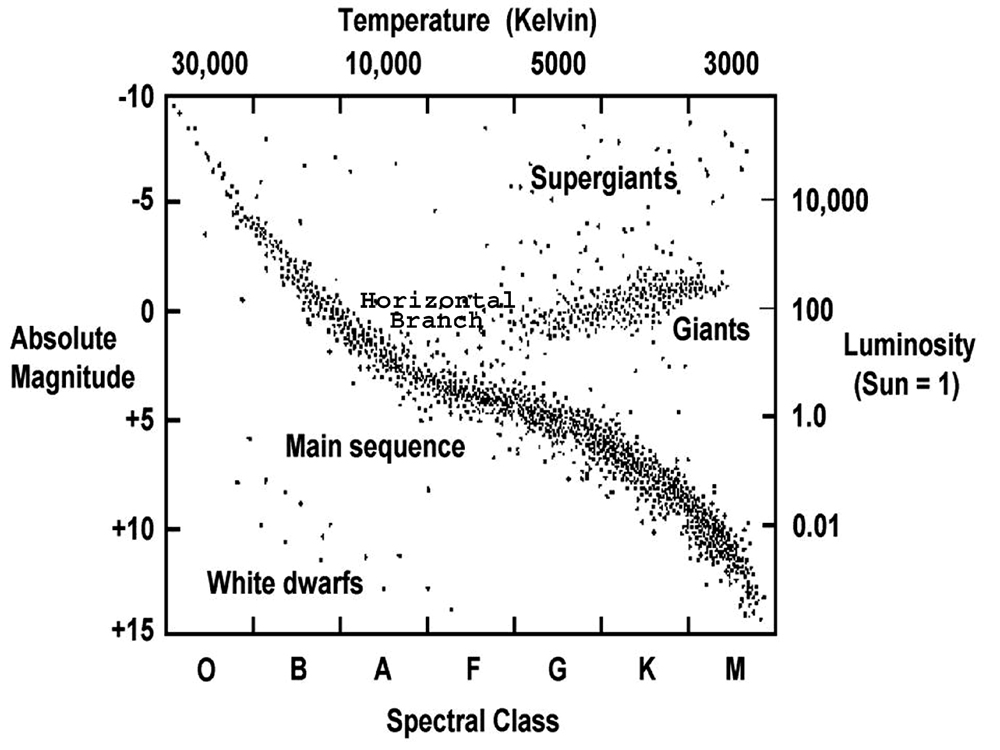
\includegraphics[width=2.5in]{fig/mainsequence.png}
% \caption{ Astronomers use  Hertzsprung-Russell diagrams to determine where is a star within the overall life-cycle of all stars.   Can we do something similar with software systems?}\label{fig:hr}
% \end{wrapfigure}
% \begin{wrapfigure}{r}{2in}
% 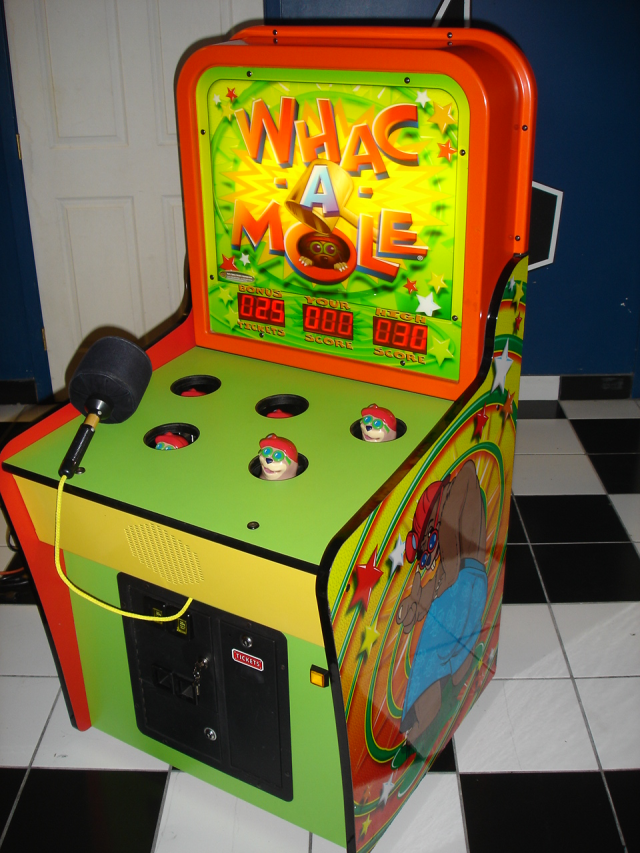
\includegraphics[width=2in]{fig/WhacaMole.png}
% \caption{ Whac-A-Mole   defenders try to
% surprise an attacker by  appearing  in different holes.}
% \end{wrapfigure}

\section{Introduction} 


``Model-based software engineering''  is where teams use high-level abstractions to guide discussion, code generation, or validation~\cite{8804427}.
Unlike document-centric
approaches, models serve as blueprints for developers to write code, and tools automate
much of the noncreative work (which translates to gains
in productivity and quality).
But
as models grow larger, it becomes harder to find  options that are most useful and most acceptable to  stakeholders.  E.g.
Section \ref{advice0} shows a seemingly simple space of options that generates trillions of possibilities.

We conjecture that    (a)
\underline{\bf if automated tools    understood stakeholder preferences and  goals} then  ~those tools can   (b)~
\underline{\bf help  development teams     explore and mature their models, faster
with   less cognitive effort}.

To check, this,   we propose
{\IT}, a tool that learns  preferences and goals from
stakeholder's ``electronic footprint'' (see examples
of that footprint in  Table~\ref{info}). \IT ~will be developed iteratively over the period of this grant.  {\IT}'s AI tools will   (a)~use  {\em large}  {\em language}  {\em models} to explore that text
\begin{wrapfigure}{r}{3in}
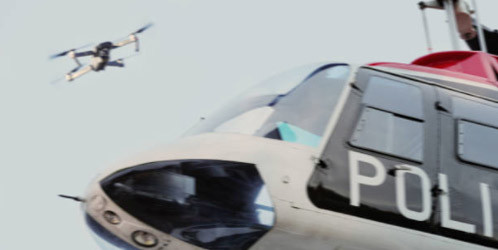
\includegraphics[width=3in]{fig/heli.png}
\caption{Model-based reasoning can find unsafe conditions
(e.g. drones   colliding      with     aircraft).}
\end{wrapfigure} 
     to infer human preferences;
 and (b)~human-in-the-loop {\em multi-objective swarm optimization } 
to help humans find the most preferred solutions
which best satisfy domain constraints.
We call this system 
{\IT}
since it takes advice    from both humans and AI. 


% \begin{wrapfigure}{r}{2.7in}
% \caption{351 options for  CS department services, inked via 510 edges (i* format~\cite{bresciani2004tropos}). }\label{cs}
% 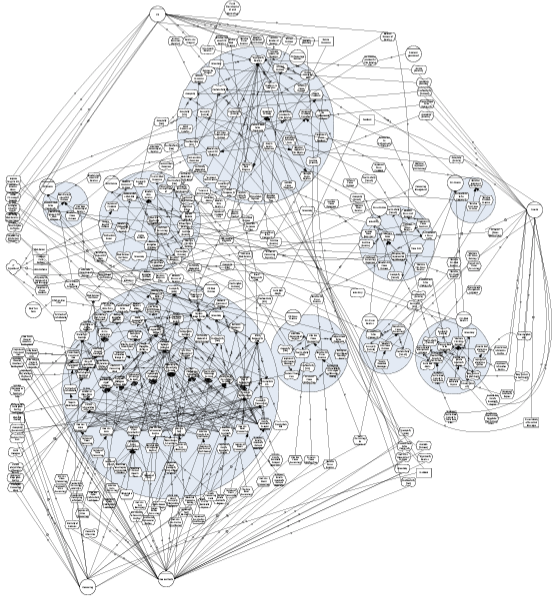
\includegraphics[width=2.7in]{fig/cs.png}
% \end{wrapfigure}

% \begin{formal}
% Combining human \& AI {\em advice} lets
% {\em teams} design and use \underline{\em model-based software}, 
% \underline{\em better} and \underline{\em faster}.
% \end{formal}
 

\begin{table}[!b]
\small
 \begin{tabular}{|p{.98\linewidth}|}\hline
 
\rowcolor{blue!10}
Team members might write opinion pieces on  Stack Overflow or medium.com 
(or other   forums), 
\\
When browsing the web, human often 
{\em lingered} longer on   pages that most interest the.  We could use  {\em lingering} to learn what
other opinions they   care about.
\\\rowcolor{blue!10}
For project under
version control, we can asee
who has commented/revised what parts of
the design.
\\
Given a version control system with comments, plus a way to register 
thumbs-up or thumbs-down ``votes'', 
we can access {\em current} and 
{\em past} decisions
of a team member.
\\\rowcolor{blue!10}
Sentiment analysis tools~\cite{novielli2015challenges}  running on text from team members
 can learn   ``hot button''
issues. \\\hline
\end{tabular}
 \caption{ Humans generate    electronic footprints that can be used   to learn    preference information.
 }\label{info}
\end{table}

This proposal will test {\IT}  on model-based software for emergency response units. 
For budgetary reasons,   emergency services   build their own drone fleets separate to each another
 (e.g.   local police
may run their own drone service). Such separate design processes    problems  when   drones have to work together   (e.g.   local, state and federal agencies called in to fight
brush fires).

To address these challenges, our tool, {\IT}, will simulate emergency services' drone models and undergo three kind of experiments. In CPU-intensive studies, we will identify hazardous scenarios, while in human-intensive studies, participants will monitor drones for off-nominal behavior. Unbeknownst to them, the simulation will enact danger scenarios identified earlier. Additionally, ablation studies will assess scenarios handled solely by AIs or humans. This forward-looking approach explores the effectiveness of human-AI interactions in managing drone-related emergency scenarios.

%To avoid those problems, {\IT} will simulate models of the  emergency services' drones.  In {\em CPU-intensive studies},  {IT} will explore the drone models to find the most interesting/dangerous scenarios. Also, in {\em human-intensive studies}, we will see how early humans can detect and repair off-nominal drone behavior.  Humans will be asked to play a simulation game where they must monitor a fleet of   drones,  watching for off-nominal situations, intervening when necessary. Unbeknownst to them, the game will then enact the   danger scenarios found in the CPU-intensive studies.  we will  also run  {\em} ablation studies where   dangerous scenarios must be handled by (a) the AIs without human input or (b) the humans without AI input

 \underline{\bf SUCCESS CRITERIA:} 
 {\IT}   will be a success if (a)~in less time, more humans can  find and explore and  assess and agree on the most
important model options;  and
(b)~the agreed upon options actually improve system performance. For example,
if an operator of a drone fleet focuses on the issues raised by \IT, they
are faster at detecting and mitigating   danger scenarios.




\subsection{Drawbacks with prior work}

 In our own experience, the best results in model-based
reasoning come from combining human and artificial intelligence advice.
For example, the model-based tool we call {\IT} addresses 
fundamental research problems   seen in  our prior work on  
the \ITS{0}
prototype. As discussed in  Section \ref{advice0},
  \ITS{0}
  found insights using {\em both}  human and  algorithmic sources 
(plus some data   mining) to reflect on the shape
of the data before deciding where to go next.
{\ITS{0}} made found better  decisions  designs  than
 state-of-the-art optimizers such as 
FLASH, HYPEROPT and OPTUNA~\cite{bergstra2015hyperopt,nair18,akiba2019optuna} 
since:
\bi 
\item \ITS{0} guided it search using human knowledge gathered at runtime;
\item  FLASH, HYPEROPT,OPTUNA use a  more
simplistic approach based on  naive random mutations.  
\ei
But even with all that,    \ITS{0} had   fundamental limitations.
While \ITS{0} did not ask questions about 
  all examples,
it can still exhaust humans with   its numerous questions. 

Also, \ITS{0} did not support debates between {\em teams} of designers
(particularly when some
of those team members have conflicting goals\footnote{How can members of the same
software development teams have competing goals? Consider the task of designing a social media tool. The security-focused team members might want elaborate authentic procedures, while the marketing-oriented team members might have much simpler, but far less secure, log-in procedures.}). 
This lack of team support is  a critical problem. As global
communications improve,   the more we can build system using  teams communicating  around the globe. In the (very likely) scenario that programmers in South America or Africa will cost 5\% to 20\%   of their North American counterparts,   many  projects will reduce their development costs by  using   teams from around the world.  In that scenario, tools like \ITS{0} would urgently need   team support.


To address this, 
{\IT} uses  stakeholders' electronic footprint (e.g. see   Table~\ref{info})
and  large language models
to automatically find the preferences of teams of stakeholders. Also, the swarm optimizers of {\IT}  will find   combinations of optiions that 
 most  overlaps with  team's preferences. That is:
\[
\textit{\IT} = \textit{\ITS{0}} +
\underbrace{\mathit{large\; language\; models}}_{\mathit{  find\; the \;preferences}} + 
\underbrace{\textit{swarm\; optimization}}_{\mathit{ uses\; the\; preferences}}
\]


 % \textcolor{red}{This is global software development..people are working together across time zones and cultures to collaborate together... they need to coordinate and communicate...but having logs can help reduce that work}
 
% \subsection{Proposed Research}
 
% To  make   \ITS{0}   team-capable, we need to make
% it smarter. The tool
%  needs more background knowledge so that it can ask  better, and fewer, questions to the design team.  In this work, we propose:

% \begin{center}
%  {\bf    Large language models (LLMs) to
%   mine team member preferences from their   {\em electronic footprints}.
% \end{center}
% As
%  shown in Table~\ref{info}, that 
%  {\em footprint}   can take many forms (social media posts, activity 
%  on question\&answering forums, browser history, comments on issues within a version control system, etc etc). Once a model-based reasoner has mined those preferences, then it can:
%  \bi 
%  \item {\em Avoid asking questions} that can be answered
%  with respect to the background knowledge;
%  \item
% {\em Shift the conclusions} towards those that are most acceptable to team members.
%  \ei
% More specifically,
% given natural language tools
% like Latent Dirichlet Allocation~\cite{Agrawal_2018} or word2vec~\cite{Mikolov13}  or BERT~\cite{Burstein19}, we will find clusters within that footprint  that characterize 
%  words  that are most liked/disliked
% by our team members.  Once the clusters are available, then we need to change tools like  \ITS{0} such that it tries to favors solutions   drawn from
%  the preferred clusters. To that end, we suggest a new variant on PSO (particle swarm optimization, see \S\ref{XXX}).  Hence, in short, our design for \ITS{1} is:
% \[
% \mathit{\ITS{1}} = \mathit{\ITS{0}} +
% \underbrace{\mathit{LLMs}}_{\mathit{  Finds\; preferences}} + 
% \underbrace{\mathit{PSO}}_{\mathit{ Uses\;  preferences}}
% \]
%  \ITS{1}  would act  like another member of the team, incrementally assessing   design options;
% sometimes asking questions; sometimes proposing compromise positions between feuding design;  as well as reporting 
%   overlooked insights.
 


% %   Given team members belonging to that
% % team for more than a few days, it would be practical for each team member to spend an hour running {\ITTT} on some small canned examples
% % that reveal that team member's attitudes
% % and preferences to across different parts of
% % the policy space within models like
% % Figure~\ref{fig:scrumModel}.\\
%  As listed in \S\ref{XXX}, there are    many research questions raised by this proposal. But at a high-level, all those questions are really different expressions of the same concern: 
% \begin{formal}
% If a model  accommodates   more preferences,
% will that  make   decision-making \underline{better} or \underline{worse}?  
%   \end{formal}  
% %\begin{formal} If models  use  extra  team and cloud knowledge,  will that  make    reasoning \underline{better} or \underline{worse}?   \end{formal}
% \noindent
% This is an important question. Clearly,   too much   divergent advice from too many sources is   counter-productive.
% As we mine a team's footprint, each  new piece of advice  is like a force that ``pulls''   the design in a certain direction. At some point, a design can be pulled in too many directions and no one's goals will be achievable.
% Hence, we   must ask   when  does  ``enough {\IT}''      become ``too much''? 


\subsection{Competencies of this Team}

This  PI and co-PI of this proposal have the experience (quantitative algorithmic reasoning and human qualitative studies) needed to succeed at this project.  PI Menzies has been working on fast algorithms for model-based SE for decades~\cite{DBLP:conf/re/FeatherM02,DBLP:journals/computer/MenziesOR07}
 and recently  had success in finding ``short-cuts''
 that allow for the rapid processing of very
 large models~\cite{Mathew17,nair18,lustosa21,lustosa22}.
 Co-PI Kuttal has extensive expertise on tool building (e.g., \cite{KuttalSSR11,tochipaper,KuttalSR13-chi}), conducting quantitative and qualitative studies (e.g., \cite{Abimgitposter2022,Diwanjiposter2022,Zhou2018,Kuttal2021, MartosKK16}), studying gender and expert based biases (e.g., \cite{Kuttal2021g, Kuttal2019, Alexposter2022, KuttalKMB21}), and mining cloud information (e.g., \cite{sarma2016hiring, KuttalCWBS21, KuttalSRW18, abs-1810-13062}). 
% Much of that has been focused on small ``lab'' problems. In this work, we explore
% that kind of reasoning, but at a much large scale.
% Specifically, we explore
% {\em the design of software for fleets
% of emergency manned and unmanned aerial vehicles}. 


  \subsection{Clarification Point: There are ``models'' and then there are ``models''}

In this proposal, we take care to distinguish two kinds of models.
  Large language models  (LLMs) are built    from sequences
of tokens from  a very large corpus. 
LLMs represent knowledge in a diffuse network  (within a neural net)-- which makes that knowledge hard to read.
On the other hand, model-based SE (MBSE) models focus on very specific domains
and are built by combinations of automatic, 
semi-automatic, and manual methods. These  MBSE models 
 use notations designed  for human readability. 
  LLMs contain much amounts of general knowledge while the MBSE models contain knowledge very specific to one domain.
Our claim is  (a) neither of these two kinds of model    replaces the other; and (b) best results
come from combining them both.  

\subsection{Scope of this Work}

Currently, we do not plan to deploy tools from this proposal into a live emergency situation. Given the safety-critical nature of emergency situations, we would have to first prove the value of our tools before any emergency service would consider using them in a live setting. Hence, this proposal.

That said, if our tools mature to that point, we would look for opportunities for live field tests.

% \subsection{Structure of this Proposal}

% The rest of this proposal is organized as follows. \cite{XXX}

 
 



% Recently we have had been exploring this problem as automatic   search-based SE optimization and  configuration problem.
% The task if multi-objective since different stakeholders usually
% make different decisions about the relevant importance of different
% test cases and use cases.
% In those tools, stakeholder preferences are
% stated before those algorithms run. The algorithms then return a set of solutions
% that attempt to trade-off between those initial preferences.
% \subsection{Terminology and Scope} 


 
% \bi
% \item
%  By \underline{\em footprint}, we mean the information
% in Table~\ref{info} comprising all the extra web content
% that can better inform us about the context of some piece of software.
% \item
% By \underline{\em stakeholders} we mean anyone who cares about the software design such as  
% managers, developers, U/IX designers, lawyers (auditing a design for discrimination), and members of emergancy response groups trying to understand and improve what is going on in a model.
% \item
% By \underline{\em team}, we mean a group of up to a dozen {\em stakeholders} arguing about some software,
% \item
% or its design. {\ITS{0}} refers to a system with {\em no} team or footprint knowledge.

% \item
%   This proposal is focused on \underline{\em  requirements engineering} (RE). RE
%  used  to happen before
% analysis, design, coding, and testing (and for mission-critical applications, there is still
% a pressing need for this to occur   before   coding starts).
% But in  the age of DevOps and Autonomous/self-adaptive systems and Software 2.0, requirements can be explored many   times in a software project\cite{Ramirez2012,ReqAwareness2010}. Hence, after Bencomo et al.~\cite{9662414}, we say
%  {\em ``Requirements engineering is any discussion about what to build and  how to
% trade-off competing costs/benefits. It can happen before, during, or after runtime~\cite{9662414}.''}. 
% \item
% \underline{\em Search-based RE}   seeks optimal or near optimal solutions in a search space of candidate solutions, guided by a fitness function that distinguishes   better and worse solutions~\cite{search12}.
%  \item
% \underline{\em Interactive Search-based RE}    lets   stakeholders     interactively
%   offer advice  to better guide that search~\cite{araujo2017architecture}. 
% \item

%   We will explore \underline{\em model-based} RE, not "green-field" discussions.
% That is to say, 
% participants in our experiments will NOT start with some blank sheet of paper. Rather, they will change some pre-existing
% knowledge in some models.   
%  We make this choice since, in this age of the mash-up, the software is rarely built without the consideration of some set of background constraints such as pre-existing requirements, legislative or corporate policies, prior design decisions, etc.  
% \item
% In this proposal, we will focus on \underline{\em serial  RE discussions} where some design artifact (the model) is being passed along a circle of stakeholders who may update the model before passing it down the circle
% (stopping when the model
% traverses the entire circle
% without revisions or comments).
% This research project will form foundations for exploring ``parallel RE design discussions'' where N people
% debate the same version of a model at the same time (future work).
%  \item
%  While we mostly focus on requirements engineering, there are an obvious extension  
%  that  could be explored, time permitting i.e.  how to extend this work to \underline{\em minimal test suite} generation; 
%  \ei


\section{Why Study MBSE (Model-Based SE)}\label{modmode}

 

% MBSE fosters   artifact reuse and  product
% quality, while shortening time to market. Amorim et al. comment~\cite{8804427} that 
% MBSE is part of
% a long-term trend towards model-centric approaches adopted
% by other engineering disciplines including mechanical, and electrical.
 \noindent We study model-based methods since they are widely used in SE. For example:
 \bi 
 \item
 In the cyberphysical realm, it is standard
practice~\cite{8453177} to deliver hardware along with
a simulation system (often written in Simulink or C).
Developers use  that simulation  during verification. 
\item
In
 requirements engineering, 
 software product line researchers explore a space of inter-connected features in a software design~\cite{mendonca2009splot,89chen2018sampling,90nair2018finding,galindo2019automated,Kira92,hierons2016sip,el2014opti,saber2017seeding,pohl11}.  Such feature models
 can be reversed engineering from code, then used
 to debate proposed   changes
 to a system~\cite{sayyad2013optimum}.
\item
 Proponents of domain-specific languages
 argue for a systems-development life-cycle that begins with (a)~defining a domain language~\cite{fowler10_dsl},
 then (b)~modeling \& executing that system
 via that   language. Low code proponents
 then add some visual editor to allow
 for rapid changes to the model~\cite{prinz2021low}).
 \item
 Software safety researchers generate   two models: one for the system under study and another for the safety properties.   Automatic tools then check for        violations of   safety  in the systems model~\cite{holzmann2014mars,8880058}.
 \item
Models can be used for the generation of runtime
systems. This is especially useful for   automotive
and embedded systems that make extensive use of models (e.g. generating executables from Simulink~\cite{mader2013oasis}).
\item 
Researchers in search-based
software engineering (SBSE) explore   models with sets of goals that may be  competing.
We have applied SBSE to models
of cloud-based architectures~\cite{chen2017riot}  (looking for ways to reduce the cost of the overall design);
NASA spaceships~\cite{DBLP:conf/re/FeatherM02} (looking for cheaper satellites that can handle more error conditions);
video encoders~\cite{nair18tse} (looking for better and faster
compression control parameters);
software process models (looking for   more functionality, at less cost) \cite{sayyad2013scalable}. % REMOVED: sayyad2013scalable
% \item
% One problem with us models was ensuring that the model corresponded to the domain it is modelling. One way to avoid that problem is to assemble the model from pre-exiting parts that are known to effect the domain. For example, Amazon Web Services
% parses the configuration files of their web applications to generate a security model
% (which is then explored for security violations by automatic theorem provers). This tool
% is run millions of time per day at AWS~\cite{8880058}.
\ei
% One reason for the increased use of
% model-based methods in SE is the
% recent increased access
% to  cloud-based CPU farms.
% With that compute power, it becomes practical
% and simple to run many ``what-if'' queries on models. This means
% that more options can be explored before committing to one particular design.
The field of model-based SE is vast. To make progress within the scope of one NSF proposal,
 we need to focus in on one kind of MBSE; the 
 emergency manned and unmanned aerial vehicles discussed below.

 
\section{What Models to Study?  (Software Models of Emergency Response Units)  }\label{egmodel}


 

 When emergency services interact, all their systems
(which may be developed separately) must now  also interact.
For example combination of  local, state and federal agencies   must now
work together in the same region
to fight brush fires.
 This can lead to many problems,
 particularly when different kinds of aircraft
 are in close proximity.
 For example, when drones are out of sight of an operator, FAA regulations requires that some manned vehicle flies overhead to act as an air-traffic controller. 
These manned aircraft may fly as low as 500' while, at the same time, unmanned drones (operate by some other emergency service) can climb  as high as 400'.
Analysts working at  NASA's SMART-STEReO project  
  used
model-based simulations~\cite{hulse2021fmdtools,Walsh20} 
to determine that 
 wind gusts,   minor operator errors, or miscommunication between the services can lead to 
a collision between manned and unmanned aerial vehicles, terminating the drones (and  losing whatever    mission functionality that drone was providing). 

SMART-STEReO~\cite{hardy22}  is an experiment in building a combined 
executable model from  the  ``ConOps'' (concepts of  operations) documents
from  different  
     emergency services.
 SMART-STEREO
  represents its knowledge in    SysML~\cite{friedenthal2014practical},   an extension to the UML modeling language.
For this  projects, the  advantage of SysML is that is is widely used
(at the time of this writing, the standard SysML text~\cite{friedenthal2014practical} has over 2400 citations)
which means recruiting enough model builders for that project
is not expected to be a problem. On the other hand, SysML does
not come with a simulation engine.
For that purpose,   we will use Hulse et. al's  fmdTools kit~\cite{hulse2021fmdtools}.
A SysML  ConOps expressed
in fmdTools includes
include
requirements tables;
derived requirements flow; requirements trace matrices; requirements allocation matrices; requirements maps; high-level diagrams of mission scenario use
cases and activities. fmdTools can execute these to   produce output
like Figure~\ref{fsim}.





% this kind of simulation analysis (e.g. see Andrej Karpathy comments on Software 2.0\footnote{ Karpathy describes Software 2.0 as "agile meets AI".
% In software 2.0, development teams
% split it two. Team1 does traditional software development while Team2's job is the care and feeding of an optimizer that
% is exploring options that will soon be adopted by Team1.  For example, Team2 could use the optimizers to (a)~auto-configure the NLP tools or (b)~find good caching options
% for the data management system.  
% For more details, see \url{https://karpathy.medium.com/software-2-0-a64152b37c35}.}).
% \item 
% Hence we assert that the methods learned here will assist a wide range of optimization-based and simulation-based software development.




 Why select this case study? As shown top of Figure~\ref{fsim}, this is a domain rich with  many models-- all of which can be executed to study their interactions.
 SMART-STEReO is part of a 
is a ten-year research effort with a budget of over \$20M/year from 2024.
PI Menzies has been working with the these personnel for nearly 15 years. Hence, we can expect that  
SMART-STEReO will be a ready source of 
mission-critical
\begin{wrapfigure}{r}{4.8in}
\begin{center}
    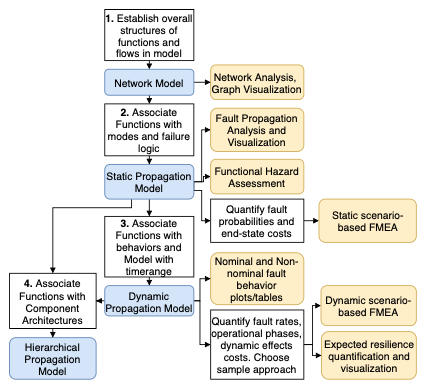
\includegraphics[height=2.4in]{fig/fmdtools.png}   
    ~ 
    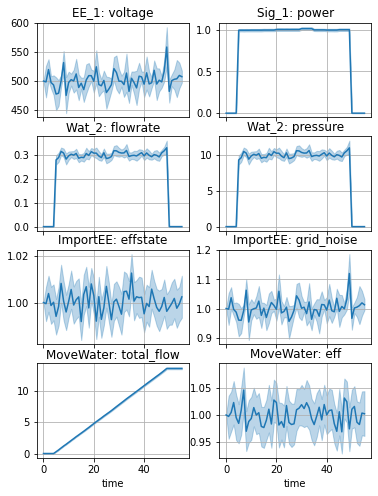
\includegraphics[height=2.5in]{fig/sim.png}
    \end{center}
\caption{Left:   fmdTools models. 
Right:  fmdTools  simulations .
From~\cite{hulse2021fmdtools}.}\label{fsim}
\end{wrapfigure} 
case study material for this project\footnote{And see also,  the ``intent to colloborate'' letter in "Additional Single Copy Documents" from that  team.}.
 Also,      the above tools     (including fmdtools) are freely available under open source licences. 
Hence, combining \IT{} with fmdtools will be a relatively straight-forward. 


Before going on we note   this proposal is not ``hard-wired'' into SMART-STEReO, SysML, or fmdTools.
From the perspective of this proposal, all the above
is just a  compiler that converts
ConOps memos into an executable (via intermediary forms within
SysML and fmdTools, that we may never need to examine in great detail).
 Once that executable is running, then the tools described  below can offer
 a general method for simulation-based analysis
 that should work for many   domains including
 drones,  autonomous cars, large cloud-based applications, and many more 

%\subsection{Why do we need more MBSE Tools?}

 
%  \begin{wrapfigure}{r}{2.7in}
%  \caption{351 options for  CS department services~\cite{bresciani2004tropos}. }\label{cs}
%   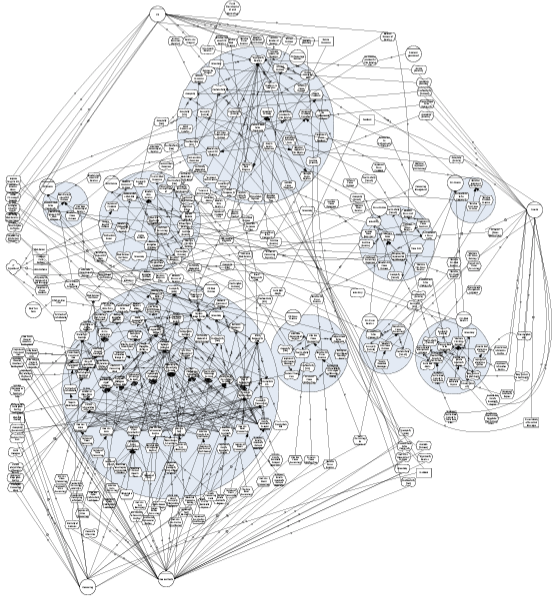
\includegraphics[width=2.7in]{fig/cs.png}
%  \end{wrapfigure}
% Why do we need more
%  MBSE tools like \ITS{1}? What is insufficient about 
%  tool suites like those shown in Figure~\ref{fsim}?

% ==> after intoructing  problems: not enough just to see them run. need to be more critical

% ==> congitive overlaod, reduce expr ost

% {\em Fourthly},
% just to answer one frequently asked question about this line of research, we could characterize the above as a  "simulation analysis" but not a "reliability  analysis":
% \bi 
% \item
% For large complex systems,  some researchers~\cite{hulse2021fmdtools,briand22,leveson2016engineering,LEVESON2009475}
% have moved from   a ``reliability'' perspective 
% (that might, say, proves properties over the source code)
% towards a  ``systems'' perspective where system properties   are   inferred from  large scale simulations   over  a wide range of nominal and off-nominal scenarios. Briand argued forcibly for this approach at his ASE'22 keynote, saying that the sheer size
% and complexity of these systems preclude  traditional reliability methods. 
% \item A counter position might be that any simulation analysis could miss
% a rare, but critical, condition. 
% \item That said, for the next decade we  know of dozens of analysts working at the SMART-STEREO project that will be studying materials like Figure~\ref{fsim}. As documented above, that analysis has already found critical bugs (when drones flying at 400 fits might be blown upwards to strike Cessnas  flying at 500 feet).  Further, given the current ease of access to cloud-based CPU, we anticipate a large group of developers using
% this kind of simulation analysis (e.g. see Andrej Karpathy comments on Software 2.0\footnote{ Karpathy describes Software 2.0 as "agile meets AI".
% In software 2.0, development teams
% split it two. Team1 does traditional software development while Team2's job is the care and feeding of an optimizer that
% is exploring options that will soon be adopted by Team1.  For example, Team2 could use the optimizers to (a)~auto-configure the NLP tools or (b)~find good caching options
% for the data management system.  
% For more details, see \url{https://karpathy.medium.com/software-2-0-a64152b37c35}.}).
% \item 
% Hence we assert that the methods learned here will assist a wide range of optimization-based and simulation-based software development.
% \ei 

%  For example, Figure~\ref{cs} lists the  the information needs of a university CS department~\cite{horkoff2016interactive}. In theory, this model can be explored to  find design choices that lead to satisfying the most goals for the most  stakeholders.
% But in practice, large models like Figure~\ref{cs} can be problematic. 
% This model is  so large that,
% in our   experience~\cite{mathew2017shorter}, humans are  daunted by its complexity.
% Even  automated tools   struggle to find choices that satisfy the  goals of that model;  e.g. 
% the NSGA-II~\cite{deb2002fast} multi-objective
% algorithm needs 1000s of seconds and 100,000s of evaluations~\cite{mathew2017shorter} to explore Figure~\ref{cs}. 



  

 

% Allowing  humans to effectively explore all the important potential behaviors of a software model is an open and important  issue. 
% In  
% ``Flaws of policies of requiring human oversight''~\cite{green2022flaws},
% Ben Green notes that many recent policies      require humans-in-the-loop to review or   audit   decisions from software models.  But that review process can be incomplete.
% % E.g. the  manual of the
% % (in)famous  COMPAS model (see Table~\ref{tbl:sigh}) notes the algorithm can make mistakes and advises that 
% % ``staff should be encouraged to use their professional judgment and override the computed risk as appropriate''~\cite{northe15}. 
% Cognitive theory~\cite{simon1956rational} tells us that
%   humans  use heuristic ``cues'' that lead them to the most important parts 
% of a model before moving on to their next
% task. But when humans review models, they can miss important details. Such cues are essential if humans are to tackle
% their busy workloads. That said,  using cues can introduce errors:
%    {\em 
%    ...people (including experts) are susceptible to ``automation bias'' (involving)  omission errors—failing to take action because the automated system did not provide an alert—and commission error}~\cite{green2022flaws}.
%  This means  that   oversight policies   can lead to the reverse of their desired effect  by {\em ``legitimizing the use of   faulty and controversial algorithms without addressing (their fundamental issues''}~\cite{green2022flaws}. 





%.  

%Cognitive theory~\cite{simon1956rational} tells us that humans  use heuristic ``cues'' that lets them find    (hopefully)  most important parts of a modelbefore rushing off to their next task.


 
%   Unfortunately,
% there are substantial examples where human oversight missed important software properties. For example,  it took years to realize that the
% COMPAS recidivism model\footnote{Used  to predict   probability of criminal behavior in the near future. Errors in COMPAS means  the wrong people are sent to jail.}
% had an alarming difference in the false alarm rates for black and white defendants~\cite{Chakraborty2020artifact}. That difference is a bug (since it can be fixed-- see PI Menzies' FSE'21 paper~\cite{fse21} that weights training examples to reduce COMPAS's false alarm delta, while  maintaining the same levels of recall on actual recidivism).

%That difference is a bug (and we know that is a  bug since it can be fixed-- see PI Menzies' FSE'21 paper~\cite{fse21} that weights training examples to reduce COMPAS's false alarm delta, while  maintaining the same levels of recall on actual recidivism).


% \begin{table}[!b]

% \small
% \begin{tabular}{|p{.98\linewidth}|}\hline
 
% \rowcolor{blue!5} The COMPAS recidivism models  labels black defendants as future criminals at twice the rate as whites~\cite{Machine_Bias}.
% \\
% Widely-used face recognition software   predicting    gender \& age, has a much
% higher error rate for dark-skinned women compared to light-skinned men~\cite{Skin_Bias}.
% \\
% \rowcolor{blue!5} Amazon's   software for same-day delivery to prime users  became   biased against black neighborhoods \cite{Amazon_Bias}. 
% \\
%   Google Translate  has gender bias. ``She is an engineer, He is a nurse''   translated to  Turkish then
%   back to  English gives ``He is an engineer, She is a nurse'' \cite{Caliskan183}.\\\hline
% \end{tabular}
% \caption{ Example biases seen in   software decisions. For more, see
% Rudin~\cite{rudin2019explaining}, 
% Nobel~\cite{noble2018algorithms},    Gebru~\cite{gebru21}.
% }\label{tbl:sigh}
% \end{table}


% To forge an effective partnership, humans and artificial intelligence (AI) need to understand each other's strengths and limitations. The software can explore a very large space,
% on pre-determined criteria. Humans can offer novel insight, but only over
% a small number of examples.  We conjecture, that when combined,
% both can find better solutions than if either 
% worked
% separately.

\section{Managing \underline{Too Many Options} (with \ITS{0})}\label{advice0}

One issue with Figure~\ref{fsim} is the overwhelming amount of information it presents. While generating numerous models and reports from a specific domain is valuable, it becomes crucial to provide a means of navigating this vast information space. Without a structured approach to exploration, the models depicted in Figure~\ref{fsim} might, at times, cause confusion rather than bringing clarity to the domain.

%One problem with Figure~\ref{fsim} is that there is too much to look at. Generating numerous models and reports from some domain is all very well. But unless we also offer some way to navigate that large space of information, the models of Figure~\ref{fsim} can sometimes confuse, not clarify a domain.


PIs Menzies and Kuttal have been studying this
problem for many years now. That work
generated the   \ITS{0} 
prototype, described in this section.
\ITS{0} has two major limitations:
(a)~it ask humans too many questions and 
(b)~it does not supporting teams
(and the rest of proposal  describes methods to   fix those problems).

To illustrate our approach, we use the example model shown in Figure~\ref{fig:scrumModel}. This figure represents Mendonca et al.'s product line model of SCRUM, offering suggestions on how to run an agile project~\cite{mendonca2009splot}. The SCRUM model comprises 128 project management options and over 250 constraints. These constraints, such as the requirement that individual tasks must take less than 10 days of programming if sprints last two weeks~\cite{mendonca2009splot}, make less than 2\% of the choices acceptable. Each choice contains:
\bi
\item An estimated development effort;
\item A purchasing cost (non-zero for features associated with third-party libraries);
\item A count of defects observed in past developments;
\item
A `success' number that increments if this node was used in a prior successful project.
\ei
When reasoning over
Figure~\ref{fig:scrumModel}, the goals are to   {\em minimize} 
the sum of 
(a)~cost, (b)~effort, and (c)~defects, while {\em maximizing}
the sum of 
the (d)~features delivered and (e)~the `success' score.  
However, finding solutions satisfying all these criteria 
 within a space
 of $2^{128}$*2\% possibilities  poses a significant challenge for humans~\cite{lustosa21}.  

 
   
\begin{figure}[!t]
\hspace{8mm} 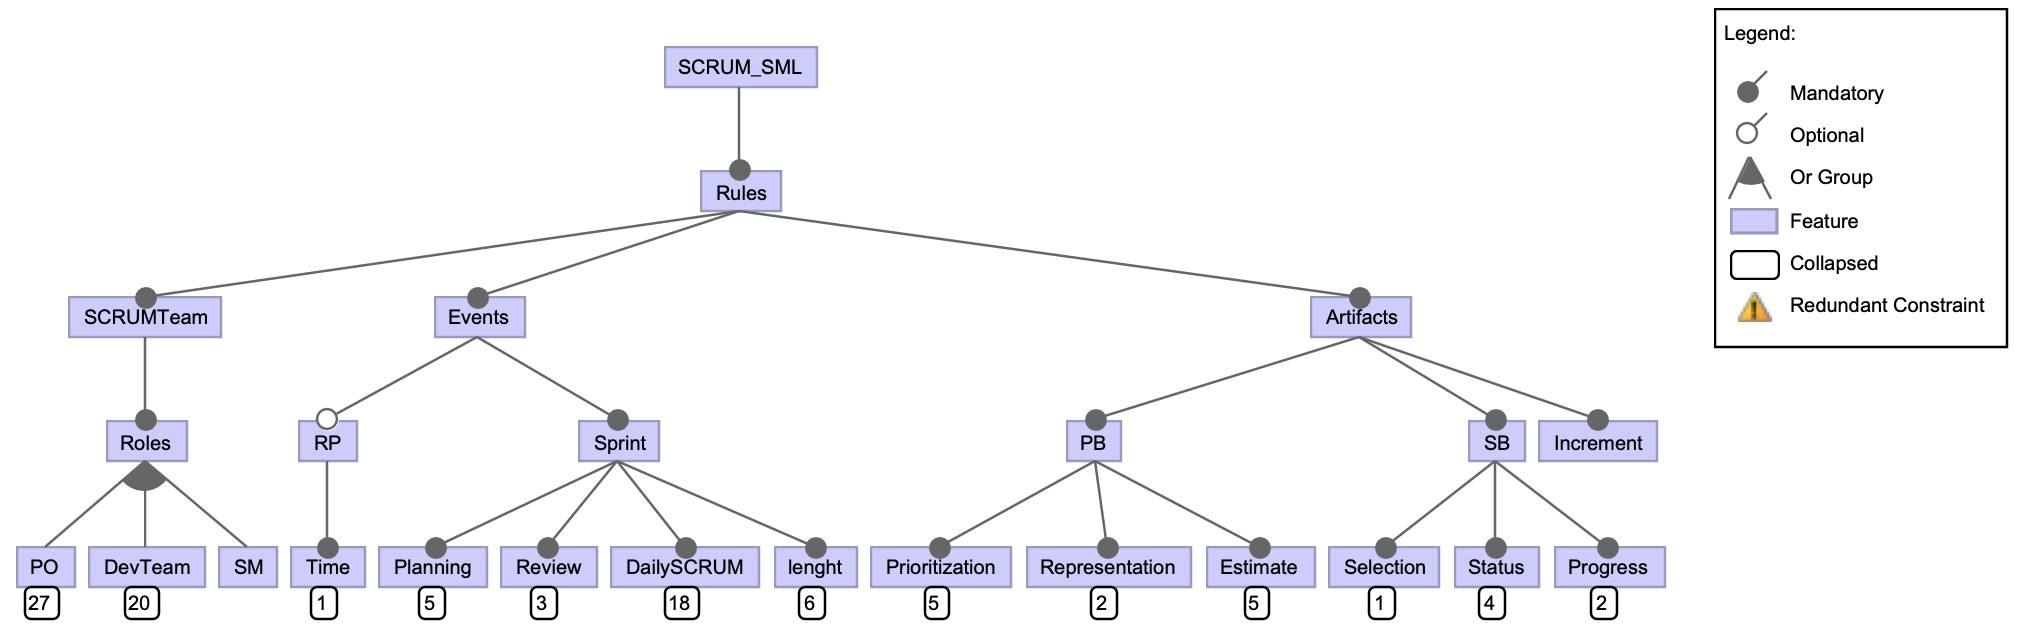
\includegraphics[width=.83\textwidth]{fig/scrumModel.png}
  \caption{{\small   SCRUM Feature Model.
 Numbers on   leaves show \#constraints in that part of
  the model. Not shown here, for space reasons, are   ``cross-tree constraints''
 that connect choices in different sub-trees. }}
  \label{fig:scrumModel}
\end{figure} 


When exploring
 too many possibilities,
AI tools like 
the PicoSAT~\cite{biere2008picosat} SAT solver can find tens of millions of satisfying solutions to Figure~\ref{fig:scrumModel}.
But now there is a new problem: \underline{\bf too many options}.

 
 \begin{table}[!b]
\small
\begin{tabular}{|p{.98\linewidth}|}\hline
\rowcolor{blue!5}
 {\ITS{0}} builds a binary tree of clusters from    $X$ examples. The {\em diversity} $D$ parts of that tree is the sum of the diversity of the $x_i$ columns  in that subset (for numerics and symbolics,  this is
 variance and entropy, respectively).\\ 
 The diversity of subtrees
$t_1,t_2$ is $D(t_1)+D(t_2)$. 
  {\ITS{0}} asks   questions
 about {\em most divisive} splits; i.e.the  largest splits with lowest diversity.\\
\rowcolor{blue!5}  {\ITS{0}}   asks about features that pass   {\em feature selection};
 i.e.   those  most distinguish       two sibling  splits.
 \\
 After asking the user  what   $x_i$ values they prefer, 
 {\ITS{0}} deletes the less preferred  half, then
 loops to the  next most divisive   split (stopping s when $N=|X|$ options has been reduced to $n=\sqrt{N}$).
 Importantly, it does so with zero calls to $f$
 (though it has had to ask the user a few questions about some $x_i$ features).\\
 \rowcolor{blue!5}These   $n$ values are  further  pruned by a   post-processor 
   that (a) finds two distant $a,b$  vectors; (b)  runs $f$ to find the   $a$ and $b$; (b) recurses on    half the data nearest the best of  $a$ and $b$ value (stopping when at $\sqrt{n}$ of the data).
   \\ 
    To decide which of $a$ and $b$, we apply the Zitzler~\cite{zit02}
   continuous domination predictor to the $y$ values of those vectors.
   This  predicate   favors  
$a$ over $b$  model if jumping from $a$ ``loses'' most:
 \begin{equation}
 \label{eq:cdom}
     \begin{array}{|l|c|r|}\hline
        \textit{worse}(a,b) =\textit{loss}(A,B) > \textit{loss}(a,b) &
        \textit{loss}(a,b)=\sum_{j=1}^n -e^{\Delta(j,a,b,n)}/n   &
        \Delta(j,a,y,n)=w_j(y_j^a  -  y_j^b)/n\\\hline
   \end{array}
    \end{equation}
where ``$n$'' is the number of objectives and $w_j\in \{-1,1\}$ depending on whether we seek to maximize goal $x_j$ and $o_{j,A}, o_{j,B}$ are the scores seen for objective $o_j$ for $A,B$, respectively.
  Zitzler   preferred ``boolean domination'' (one thing is better than another if it is no worse on any criteria and better on at least one criterion) since, it is known that boolean domination can  fail for three or more goals~\cite{Wagner:2007, Sayyad:2013}.
   \\    \rowcolor{blue!5}  Post-processor needs $2log_2(n)$ calls to find
   $\sqrt{\sqrt{N}}$ options that   survived   the tree pruning
   {\em and} the post-processing.\\\hline
 \end{tabular}
 \caption{\ITS{0} automatically finds cues that guide to better solutions.
  Later in this proposal, we will
assess the value of (a)~automatically finding cues
versus (b)~surveying humans to find their cues.
}\label{advice1}
\end{table} 
 
 \ITS{0} was an experiment that used human preferences to reduce
that space of too many options.
{\ITS{0}}  worked with humans, asking them the least number of questions to find good solutions~\cite{lustosa21}.
 {\ITS{0}} applied
the data mining operators 
of Table~\ref{advice1} to find cues that    select for good solutions most acceptable to participants (where those cues rule out the most number of the remaining options, so that very few questions are needed to be asked next).
Those operators include
(a)~random projections to recursively
  bi-cluster the data; (b)~entropy measures to assess
  which clusters should be explored first;
  (c)~semi-supervised learning to cluster the space, then ask only a few questions
  per cluster;
  (d)~feature selection to select which attributes are most informative. 
  For details, see Table~\ref{advice1}.
  
  {\ITS{0}} is an active learner~\cite{settles2009active} that decides between options $X=\{x_1,x_2,..\}$,   scored
by a human $f$ on goals $y_i$, so   $y_i=f(x_i)$
(where $x$ are (e.g.) 128 decisions within the model of Figure~\ref{fig:scrumModel}
and   $y$ are 
multiple objectives
such as
``Minimize size of team''  or
``Deliver more product sooner'').
 {\IT} assumes that is 
 \underline{\bf   expensive} to call $f$ (since each such calls means
pestering a human for an expert opinion) but
  \underline{\bf   cheap} to find   many $x_i$ vectors (e.g.  random   selection over  10 binary options
  generates  $|X| \le 2^{10}=1024$ options). 
   
  
  

  
 

 
 
  


Just to highlight the benefits of our approach, we note that
when {\ITS{0}} asks  a question, we \underline{\em do not} mean users
are asked to pick between
two   lists of the 128 features in 
Figure~\ref{fig:scrumModel} (since  users would quickly   tire of those kinds of questions).
Rather, when we say ``{\ITS{0}} asks the users for a question'', that question asks for preferences amongst the {\em fewest} features that {\em most} distinguishes clusters within the current space of options.
In this way, answers to each question can quickly wipe out large sections of the search space,
thus reducing the number of subsequent questions we will ever need to  ask.



 As said above,
in studies~\cite{lustosa21} with a dozen SE    models,   \ITS{0} cued into solutions within 1\% to 3\%
of optimum after asking humans 10 to 100 questions. 
The decisions found by \ITS{0}   
out-performed state-of-the-art optimizers such as 
FLASH, HYPEROPT and OPTUNA~\cite{bergstra2015hyperopt,nair18,akiba2019optuna}. We conjecture
 that those
other optimizers before performed worse
since they used a somewhat uninformed
search based on  random mutations.
On the other hand, 
\ITS{0} works   so well since
   (a)~it combined insights from {\em both} human and algorithmic sources and (b)~using the data mining operators defined later in this proposal (see
Table~\ref{advice1}), it reflected the shape
of the data before deciding where to go next.

 
 




% For example, working with humans, our  \ITS{0} software tool~\cite{lustosa21,lustosa22}  explores
% trillions of options to find a few, most important,
%  decisions that give the best results from a model.
%   {\ITS{0}} takes advice from humans-- but only sparingly. In studies with a dozen SE models {\ITS{0}} cued into solutions within 1\% to 3\%
% of optimum after asking humans 10 to 100 questions (and prior state-of-the-art
% tool~\cite{araujo2017architecture}, which used stochastic evolutionary   algorithms, needed $1,000$ to $100,000$ questions to get equivalent
% results). 
% Interestingly, the decisions found by \ITS{0} out-performed state-of-the-art optimisers such as 
% FLASH, HYPEROPT and OPTUNA~\cite{bergstra2015hyperopt,nair18,akiba2019optuna}. We conjecture that those
% other optimisers performed worse
% since they used a somewhat uninformed
% search based on  random mutations.
% On the other hand, 
% \ITS{0} works well
%  because (a)~it combined insights from {\em both} human and algorithmic sources and (b)~using the data mining operators defined later in this proposal (see
% Table~\ref{advice1}), it reflected the shape
% of the data before deciding where to go next.

 

% \textcolor{red}{remove this}Another reason to fund this proposal is that while the combination of tools used here 
% is novel, this team already has extensive experience with many parts of this assembly~\cite{mathew2017shorter,fse21,Agrawal_2018,majumder2018,Agrawal19z,MenziesM08}\footnote{E.g.  
% Our bias mitigation work~\cite{fse21} won ``distinguished paper'' at FSE'21.
% \cite{MenziesM08} was honored as a distinguished ``test of time'' paper at ICSME'19.  Our algorithms can optimize Figure~\ref{cs} 100s of times faster than NSGA-II~\cite{mathew2017shorter}. \cite{majumder2018} showed how to speed  up reasoning over cloud knowledge
%   (by three orders of magnitude). \cite{Agrawal19z} discussed methods of how to very quickly tune and improve the NLP techniques need to analyze cloud textual data.}.



% Building and reflecting over domain models is a widely used practice in
% SE. Such models may be described in some informal manner (e.g. scribbles on a whiteboard, notes on a napkin), some may be added to redesign documents to clarify that discussion, some actually have formal semantics and can be processed by theorem provers. Regardless, participants in a design process over take the time to draw, share, review and discuss some form of model. 





% Increasingly,   society is organized by software. To avoid problems like
% the software-induced decision biases listed in Table~\ref{tbl:sigh}, 
% we urgently need    tools that better understand and respect the goals 
% of humans.

% To address this issue, we propose the {\IT} project-- an interactive search-based
% SE (SBSE) approach that uses extra ``advice'' about
% what humans like (or need) the   most (or least).  SBSE seeks optimal or near optimal solutions in a search space of candidate solutions, guided by a fitness function that distinguishes   better and worse solutions~\cite{search12}.
% {\em   Interactive SBSE}  (iSBSE) lets human stakeholders     interactively
%  offer advice on how to better guide that search~\cite{araujo2017architecture}.
%  {\IT} uses iSBSE and data miners to ensure
%   users are asked the fewest,  most informative, questions. 

%  To impleme 


%  Note that all would benefit not just {\ITTT},
%  but also    other   model-based reasoning processes.
% Human and AI   could work together better  since they can now access and explore each other's goals.  


% \begin{table} 
% \caption{ Some of the drawbacks with {\ITS{0}}. While there may be more than just the ones listed here, within the space of this NSF
% grant, we elect to focus on the following issues.}\label{info}
% \small\begin{tabular}{|lp{5.55in}|}\hline

% \rowcolor{blue!5}Congitive&{\ITS{0}}  trusted the answers it collected from humans.
% But human advice can be faulty. How can {\ITTT} recognize
% faulty answers and how to mitigate the negative
% effect of those faults?
% \\

% Cognitive& 
%  {\ITS{0}}  only takes advice from one person--
% which means its conclusions can be unduly biased by the views
% of one person.
% {\ITTT} should listen to teams of people working some problems.
% But humans can be argumentative.
% If we accept   advice from multiple humans, will
% all that advice help or hurt {\ITTT}'s processing?  
% \\\hline
%\rowcolor{blue!5}
% Social &  Table~\ref{tbl:sigh},
% software-based decision making can exhibit bias.
% Models may attributes describing ``projected
% groups'' with special privileges (or, sadly, lack of privilege). For such models,  bias manifest when 
% the performance of a model is significantly different for different groups.
%  {\ITTT} needs bias motoring and bias mitigation operators
% to   adjust conclusions in order to better  empower   the disempowered
% sections of society who (usually) are not included in software design discussion.  
% \\
% \hline
% Negotiation & 
% If we listen less to AI and more to humans, does that mean we have to compromise our optimization
% goals in order to appease more people?  \\
%\rowcolor{blue!5}Negotiation & How much advice is too much? At what point do we need to just give up since there are too many different competing forces   to optimize the model? And in the space before we have to give up, are there still useful modeling challenges?
% \\\hline
% Engineering & How to collect the advice in a cost-effective manner?\\
% \rowcolor{blue!5}Engineering&  Does this extra advice change the
%   reasoning?\\
%  Engineering  &{\ITS{0}}   adjusts its conclusions based on feedback from the people it talks to. 
% If, at some later time, some oversight group wants to
% know {\em why} some solution was reached, they may not
% have access to the humans who guided the original search (e.g. they may not recall why they made that decision and/or they have left the organization).
% So how can {\ITTT} give oversight bodies the information they need
% to audit past decisions? And how to do that in a cost-effective manner? \\
%  \rowcolor{blue!5}Engineering&   {\ITS{0}} used a set of tactics to guide its question asking. There are   many such tactics and {\ITS{0}} just
% explored the tricks of Table~\ref{advice1}. 
% {\ITTT} needs to explore that larger space of (many)  different tactics for reducing human workload.  \\\hline
% \end{tabular}
% \end{table}

 
 
 

% Green   mainly refers to software addressing  legal or corporate issues.
%   But 
%   a similar story can be told about many aspects of software engineering:
%   \bi
%   \item
%   Requirements engineering can go astray when the views of one class of stakeholder
%   dominate the design, or the combination of user viewpoints becomes too complex to
%   negotiate~\cite{mathew2017shorter}.
%   \item The design of data structures is incomplete when humans overlook
%   an important use case~\cite{Jacobson87}. 
%   \item Test generation is incomplete when the  test  generator  
%   (some mixture of human or automatic methods) ignores
%       critical parts of the program~\cite{miller90,fuzzingbook2021}.
%   \ei
%   In this context, it is useful  to note the  rising interest in ``Software 2.0''~\cite{ratner2019role}
%   where development teams split into (a)~a team of standard developers and 
%   (b)~a second AI-based team running
%   large scale what-if queries through some optimizer.   Software 2.0
%   makes it faster to explore more design options  such as (e.g.) how to configure the learner inside a vision system ~\cite{karpathy17}. On the other hand,  amongst
%   the space of explored options, it is hard to tell if Software 2.0 is exploring
%   (or missing) all the important options.
 
   
   




%  \subsection{Advantages of this approach}
%  This proposal will use   models like Figure~\ref{fig:scrumModel} for its reasoning.
% In defence of that   decision, we note that the above    example is a  specific instance
%  of      \underline{\bf a very general
%     process}.
%      {\ITS{0}} has been seen to work for a wide range of models. The same paper that reported on the SCRUM model study found similar results
%  (that {\ITS{0}} was more effective than other iSBSE tools) in nine other models.
% In other work~\cite{lustosa22},
% {\ITS{0}} found   solutions  competitive with state-of-the-art optimizers
% While 
%    other tools had to ask
%  thousands of questions,  {\ITS{0}} only had to ask dozens.
 
%  Also,
%     the visual forms used here   are {\em feature models} which offer a simple succinct high-level tree-like view  of  very large systems (for example, see Figure~\ref{fig:scrumModel}). They are human browsable and modifiable.  Hence, the original 1990 paper on feature models~\cite{kang1990feature}   has 5,535 citations (as on May31,2022).
%     One measure of the generality   is how
%     widely a framework is   used.    Feature models have been
%      used for a very large number of SE tasks\footnote{
%     Configuring LINUX    kernels~\cite{Sayyad13};
%     software reuse~\cite{Medeiros21,NOGUEIRATEIXEIRA2019106175},
%   software traceability~\cite{batot2022survey}
%     software project management~\cite{lustosa21}, defect prediction~\cite{Bhushan20}, and design pattern discovery (i.e. looking for repeated patterns within part of different designs~\cite{Thaller}), etc.} and,
%     on the web,
%     we can access 100s of large   models of this format\footnote{See \url{https://github.com/marcilio/splot-research/tree/master/SPLOT-Research/WebContent/models}  for feature models of problems as diverse as the design of electronic shopping carts, different software security authentication schemes,
%     and operating system designs.}.
  
%    Another reason to use feature models is that they can be given   a precise semantics. Automatic tools exist to convert these tools into conjunction normal form. For example, Figure~\ref{fig:scrumModel} translates in to 256 clauses which then be processed by SAT-solved like PicoSAT~\cite{biere2008picosat}.
%     When the literals in those models are augmented with numerics like ``time required to implement this in prior developments'',
%     or ``number of bugs previously encountered in this feature'' then
%     multi-objective optimization tools (like {\IT}) can  perform large-scale trade-off studies between different options\cite{Sayyad13,lustosa21,lustosa22};.
    
   %  More importantly for this proposal, 
    

\section{How to do it, better? }\label{better}
 As stated above, our prior work with ADVICE-0 did not support teams and asked too many unnecessary questions. Here, we propose (a)~adding team support via {\em swarm optimization}; and (b)~using
 smarter (and fewer) questions, generated   via {\em large language models}.

%  \begin{wrapfigure}{r}{2.1in}
%   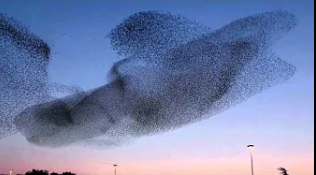
\includegraphics[width=2.1in]{fig/starlings.png}
% \caption{Birds solving problems by
%  loosely connected, actions.}
% \end{wrapfigure} 
%  As stated in our introduction, while it was a promising first step, \ITS{0} has some major drawbacks.
%  Firstly, in its current form \ITS{0} takes advice from one, and only one human. To
% become team-capable, it must be able to handle debates.
% Secondly, \ITS{0} can pester humans with too many questions; e.g. in the above
% studies, 10 to 100 questions. While 100 questions may not sound excessive, it can take days for teams to agree about just a few dozen   examples\footnote{Evidence: 
% In ``Heuristics for systems engineering``, Vilardi et al.~\cite{valerdi2010heuristics} report experiments with Delphi panels where a group of ten experts meet each day to discuss examples containing two dozen attribute.  The group meet every day until their views converged. It took
% this team 3 meetings of two hour each to assess 50 examples}.  

 
 
% The remainder of this proposal discusses ways to address the problems.
%  In summary,
% instead of
%  making a single
% conclusion,  \ITS{1} will use   swarm optimization (described below)
%  to give each stakeholder $N$ swarm particles, all of which will     debate  where to find good solutions.
% Also, instead of asking humans every question, we answer most of them
%  using background knowledge learned
%  from the electronic footprint of Table~\ref{info}.
 
\subsection{ Adding Team-based Reasoning (using Swarm Optimization)}\label{teams}


 \begin{wrapfigure}{r}{1.8in}
 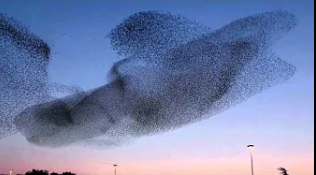
\includegraphics[width=1.8in]{fig/starlings.png}
 \end{wrapfigure} 

 
 At sunset in Siberia,
  flocks of starlings   fly
 in beautiful patterns called a murmuration.
 This complex    behavior has no centralized controller but arises from many
  local decions based on   feedback from   neighbors.
 
Inspired by these starlings,
researchers in {\em particle swam optimization} (PSO)~\cite{kennedy95particle} view
optimization   as   a set of candidates
``flying around''
(i.e.   being mutated)  a shared space. 
  This  scheme  lends itself naturally  to a group performing model maintenance. In PSO, particles do not just arrive at some location and stop. Instead, each particle is like a   helicopter buzzing around the landscape. 
 New model conditions are like a breeze that pushes the particles   some distance across the decision space in a model.  Our particles then must make new decisions as they   negotiate their way back to their preferred positions.   
 
 \begin{wrapfigure}{r}{1.7in}
  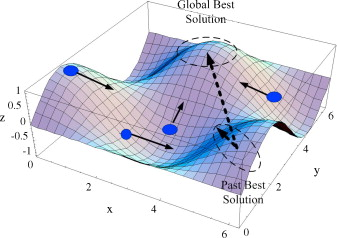
\includegraphics[width=1.7in]{fig/pso1.png}
\caption{Particle Swarm \\Optimization.} \label{pso1}
\end{wrapfigure} 
We argue that 
 PSO is  a natural method for negotiating  shared solutions.
Particle velocity   is controlled by     
{\em inertial},   {\em cognitive}, and  
{\em social} weights $w,\phi_p,\phi_g$ 
(where {\em p, g} are short for ``personnel'' and ``group'').
In a swam of ``particles'' $p$ 
 ``flying around''  
(i.e. being mutated across a set of vectors),
then:
\bi
\item
The $w$ 
{\em interia} factor pushes   $p_i$ along the  
current direction. 
\item
While  the {\em cognitive} and 
{\em social} weightings 
$\phi_p,\phi_g$ pulls $p_i$ towards
(a)~the best solution found by this
particle or (b)~the best solution found by the entire
swarm of particles. 
\item
  $w,\phi_p,\phi_g$ serve to  nudge
  $p_i$ to a new direction.\ei
 
 PSO's particles  find a balance between   past decisions ($w$), the preferences of one explorer 
($\phi_p$), and the preferences made by the team ($\phi_g$).
In our scheme,
  stakeholders  gets multiple particles, initialized to:
\bi
\item An initial random  position within the space of options.
\item Or, if the crowd knowledge is available (see next section), 
positioned  amidst the crowd knowledge.
\ei
Initial particle velocity is  set according to how far, and in what direction, are the ideal answers for each individual (the further  you start from your ideal, the more aggressively you jump towards it). 


 To prepare for this proposal, we built a simple PSO 
for Figure~\ref{fig:scrumModel}. That tool needed   10,000s of evaluations. If each  evaluation is one   question, then this would  be  overwhelming for human users.
 
To reduce that problem, we take inspiration from a
2021 paper by Mai et al.~\cite{MAI2021398}. They 
used PSO  
with the evaluation oracle replaced with   fuzzy c-means clustering (FCM)\footnote{In FCM, examples
may appear in   multiple clusters. Membership probabilities are
computed by iteratively updating  a matrix of membership values   using
values from the last iteration-- then repeating until convergence is reached.}.  When  FCM needs labels, it computes them from  a weighted sum of the labeled examples in   nearby clusters.  While an exemplary approach in many respects Mai et al.'s design  still makes 100s to 1000s (or more) queries
to some oracle. To make PSO palatable for humans,
    we adapt  Mai et al., replacing fuzzy c-means with the methods of  Table~\ref{advice1} (i.e. {\ITS{0}}
    will be a small sub-routine inside {\IT}
    In this way, humans would   only be bothered
    for their opinions on a small number of   most  critical questions.

 \subsection{ Additional Knowledge from the Electronic Footprints (using LLMs)}\label{cloud}
% The {\ITS{0}} 
%  experience~\cite{lustosa21,lustosa22} was that,   apart from the $y$ goals,
% users have numerous   preferences within the $x$ space  of decisions over   matters like ``what tools to use in development'' or ``what size of team most suites their personnel development style''.  Specially, in our prior experiments with {\ITS{0}}, we  found users with  one to two dozen such $x$ value preferences for the options with Figure~\ref{fig:scrumModel}.
% To handle these $x$ preferences, we cannot just add them to the $y$ goals since this would
% lead to an too many goals.
% Hence, for   $x$ preferences, we need   another approach.




\begin{wrapfigure}{r}{2.25in}
  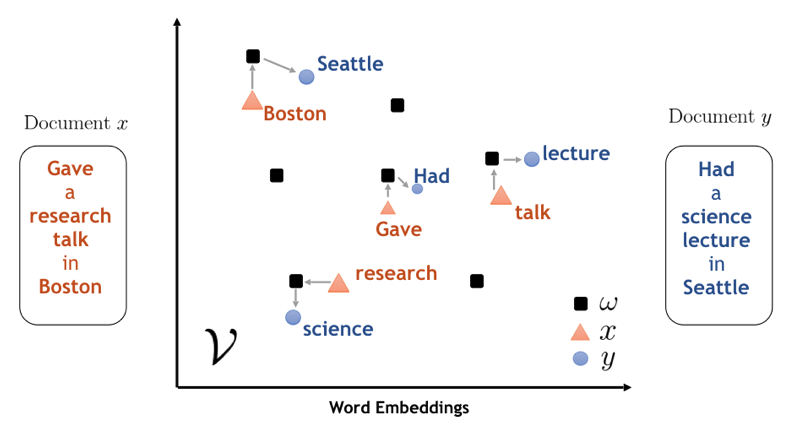
\includegraphics[width=2.25in]{fig/word2vec.png}
\caption{Encodings to find synonyms.
From  IBM: blogs/research/2018/11/word-movers-embedding/.\vspace{1mm}}\label{aka} 
\end{wrapfigure}
With \ITS{0} ~\cite{lustosa21,lustosa22} we found that many preferences about $x$ decisions
are ``soft''; i.e. open to negotiation;
e.g. a developer might say ``I prefer     C, but I can code in C++   if you need me too.''. 
To handle  soft goals, we propose
adding a new preference
term $\phi_x$ to
the set $w,\phi_p,\phi_g$ that controls the
PSO.    The PSO we propose has
different particles assigned to different stakeholders;
and an extra term $\phi_x$ that nudges particles toward/away from things that this stakeholder likes/dislikes. 

 To find  preference knowledge, {\IT} would explore the electronic
footprint of   team members (see Table~\ref{info}). 
 But there is a problem. The text of the electronic footprint discusses {\em old} problems which may    not overlap with the text of the {\em new} model.

To fix this, {\IT} must \underline{\bf discover synonyms} that map from
the {\em old} words (in the past) to the {\em new} words (seen in the current models).
There are many technologies that could be applied here
(e.g. see Figure~\ref{aka}). Fu et al.~\cite{Fu22} recently reported success in improving predictions using BERT to expand the
vocabulary of use case stories~\cite{Burstein19}. Co-PI Kuttal used transformer-based language models, specifically 
 BERT, GPT2, and XLNet, to classify the intent of developer conversations \cite{RobeFSE2022, Hartposter2022, Alexposter2022}.
She has also used information sources such as GitHub, Stack Overflow and App Stores to mine the technical and social skills of developers \cite{sarma2016hiring, KuttalCWBS21}, study migration behavior across platforms \cite{abs-1810-13062}, compare app user behavior (compared to developers) \cite{Kuttal2020TugOP}, and model developer foraging behavior \cite{Abimgitposter2022,Zhou2018,RagavanPPHKSB17}. 



  Given recent advances in large-language models, we say that prior
work can be significantly improved.  A preliminary analysis of the Table~\ref{info}
corpus suggests that, for any one team member, that corpus will consist of $10^2$
to $10^3$ short phrases that mention (e.g.) ``scalability'' and ``array bounds checking''.
To find the synonyms around these terms, we will use GPT-4.
\bi 
\item In GPT-4 the prompt ``what else should I know about scalability'' results in 60 lines of text containing dozens of
synonyms for ``scalability'' such as {\em bottlenecks}, 
{\em load balancing}, {\em coaching strategies}.
\item 
Similarly for ``Check for array out of bounds'' if prompted
``what else should I know about ``array out of bounds''''
yields  450 words with   synonyms like
  {\em unit testing}, {\em memory corruption}, {\em dynamic array resizing}.
\ei
We would then use sentiment analysis and Chat-GPT to see if
team members approved of those terms.
Lin et al.~\cite{Lin18} says  
{\em sentiment analysis}  finds
objective states and subjective opinions.  
Stakeholder footprints   might    
express a positive sentiment  towards   (a)~specific  social groups (women, veterans) or
(b)~verification technology that evaluates
a system.
For example, the 
ChatGPT      prompts  
``Using the text of the Agile Manifesto, do it's authors like or dislike  waterfall development?  Please answer with one word.'' results in {\em dislike}\footnote{
The Agile Manifesto~\cite{beck2001agile}, written in 2001,  outlined principles favoring flexible and collaborative approaches to software development.
Note that the manifesto does not mention the term ``waterfall''; i.e. ChatGPT worked out that connection for itself}. Interestingly, ChatGPT seems quite discerning in this task. If we run this prompt again, substituting ``waterfall development'' for ``elephants'',
ChatGPT responds appropriately with {\em neutral}.

Note that we would not ask ``what else should I know'' for all synonyms.
 Peng et al.'s GODEL system~\cite{peng2022godel}
 recommends learning by   first filtering
words by their LM loss\footnote{LM loss is the   errors made in predicting
the $n+1$-th token after seeing tokens $1,..n$.}. By sorting  on the LM loss, we can
identify words that are {\em gold} or {\em rusty}; i.e. those with the highest or lowest LM loss. Peng et al. report success after training using equal numbers of gold and rusty words-- a  result that calls to mind older work in active learning~\cite{yu2019improving} that found that
the most uncertain regions (which here would be the words with highest LM loss),
can be most useful for refining the boundary between (say) like and dislike.
 

 

%   To find the regions that users
%  want to avoid, we apply the following three technologies to the  electronic footprint discussed in  Table~\ref{info}. co-PI Menzies has   much recent success with natural language processing of SE sources such as 
% questions on StackOverflow~\cite{MenziesM08,Agrawal_2018,majumder2018,Agrawal19z}. Extending that work, we would first
% apply 
% {\bf natural language} processing~\cite{Agrawal_2018,majumder2018,Agrawal19z,MenziesM08} 
% to mine a stakeholder's electronic footprint
% of Table~\ref{info}; then
% apply   sentiment analysis  to find terms
% liked/disliked by a stakeholder~\cite{novielli2018benchmark}, then  
%  synonym discovery ~\cite{Burstein19} to map 
% terms in the electronic footprint
% to the terms of the model
% (i.e. map from the general language of the   footprint to the specifics of the model.


 






 
%  \subsection{\ITS{3} = \ITS{2} + Advice  Verification Tools} \label{verify}


 
% Given so many team
% members and so many knowledge sources, then we should expect that some team members and some knowledge sources are more useful than others. 
%  Using {\em meta-patterns of fault-less or fault-full   behavior}, we  need to distinguish and manage (a)~the   advice that is most helpful; and (b)~the     advice
%   that most   hurt our ability to satisfy more goals.  

%  One such meta-pattern is
%  {\em good advice needs less revision}.
%  Suppose we   have a version tracking system (e.g. GitHub)
%  that watches model revisions proposed by a group of stakeholders. Suppose further those stakeholders are   using  the knowledge sources from Table~\ref{info},
%  over several weeks or months.
%  Those stakeholders and/or those knowledge sources 
% can now be ranked by how often their advice is subsequently revised. Under the assumption
% that good advice is revised less,   we can   weigh our PSO explorations to favor regions  with ``good'' knowledge sources 


%     \begin{wrapfigure}{r}{1.5in}
%     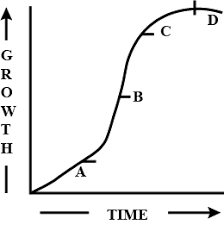
\includegraphics[width=1.5in]{fig/growth.png}
%  \end{wrapfigure}
%  Another such meta-pattern  is {\em bad advice
% means  more performance variance}.
% In a recent  TSE'21 article~\cite{8883076}, PI Menzies and his student Zhe Yu~\cite{8883076} 
%   found they could apply growth curve mathematics~\cite{camilli2022modeling} to interactive search-based methods.  At each ``time tick'', humans make some decisions and the performance scores change (hopefully, it improves).
%  As shown at right,  early on (at point ``A''), PI Menzies and Yu were able   to extrapolate forward the expected future shape of the graph. 
%  Such extrapolations fail when   bad advice   throws a project off course. In that case, a repair action could be to    {\em replay}  everything   from the nearest point where the extrapolations were predicting accurately.
% Here, by ``replay'' we mean  reset the model back to some early point {\em but keep all the answers from users
%  seen since that point}. Then apply our inference tools to see what happens if we change the answer at the early point, then try to reapply the answers seen subsequently.
  


%  Potentially, there are many other  meta-patterns such as {\em bad advice comes very quickly}
%  or {\em good advice explores more options before deciding}. We plan extensive observation of
%  our experimental participants to identify which meta-patterns are most useful.

   

%  \subsection{\ITS{4} = \ITS{3} + Bias Mitigation}\label{bias}
%  Here, we are talking about how to manage problems like those
%  seen in   Table~\ref{tbl:sigh}.
 
% To manage bias, first, we have to measure it.
% A recent literature review by PI Menzies and his student Suvodeep
% Majumder~\cite{Majumder21} lists   current metrics seen in the SE literature that report performance variance between test cases from different social groups. Many of those are for categorical values (and our  $y$-space objectives will be numeric), so we will adapt those too (e.g.) report the variance reduction if we jump to specific social groups (and the {\em more}    variance reduction means {\em more} bias). 

% Now that we can measure bias, we must mitigate it.
% Four such mitigation methods are: %{\em personnel balancing},  {\em extra context}, {\em hyperparameter optimization} and {\em sample balancing}.
% \bi
% \item {\em Personnel balancing}: As to {\em personnel balancing},
%  Leavey \cite{Leavy2018},
% Nobel~\cite{noble2018algorithms} and    Gebru~\cite{gebru21} warn that a lack of diversity in a design team   leads to designs that discriminate against particular sections of society.
% % We fully endorse Leavey,Nobel, and Gebru's call for
% % more diversity in design groups.
% % But some design teams cannot access all the   diverse personnel that they might want. E.g.
% % female   faculty in the USA are  besieged
% % with requests to join different committees\footnote{\url{https://csw.arizona.edu/sites/default/files/data/Faculty Service infographic.pdf}} (this is particularly true in SE where conference commitees strive for gender equity, but only 20\% of SE faculty in the United States are female). Hence,   junior female faculty are now advised to  ``say no more than yes'' to committee work. 
% Co-PI Kuttal in her lab studies found  that balancing helps in removing any gender and expert biases \cite{Kuttal2021g, Kuttal2019, Alexposter2022, KuttalKMB21, Robe2020}.
% Issues like that motivate us to  explore
% hybrid methods that combine personnel balancing with   other methods:

% \item
% {\em Extra context:}  Recall that that \IT{2}  expands model
% terminology using       Table~\ref{info}.  Our experiments   will check how bias is effected by increasing Table~\ref{info} information. \textcolor{black}{Co-PI Kuttal analyzing the gender data found that BERT model needs extra context \cite{Alexposter2022} while SVM models can use a gender   feature~\cite{Robe2020}.}
%  \item {\em Hyperparameter optimizers} are algorithms that      find settings for  data miners that 
%  improve predictively
%  performance. As showed in our FSE'20 paper~\cite{Chakraborty_2020},
%  that     process can also be used to select models whose output decreases
%  disparities between social groups (e.g. such as those reported in our introduction for COMPAS).
%  Accordingly,  for \ITS{4}, we would
%    revisit that FSE'20 work to  find even better Hyperparameter optimizers for PSO that remove even more disparity between social groupings. 
% \item
%  {\em Sample balancing} mitigates bias   arises from an imbalanced
%   sampling of   social groupings by 
%   adjusting the ratios of those   groupings (within the sample
%   used to build a model).
%   At  FSE'21 PI Menzies
%  and his student  Joymallya Chakraborty earned a distinguished paper award~\cite{fse21} 
%  for a system that extrapolated examples within under-represented social groups within the training data\footnote{Implementation note: that system adjusted frequencies in the 
%  {\em training} data and {\bf NOT} the {\em test} data.}.
%   Prior to that work, it was  feared   that repairing bias also meant damaging predictive efficacy\footnote{
% In 2017,    Berk et al.~\cite{berk2017fairness}   said
% "It is impossible to achieve fairness and high performance simultaneously (except in trivial cases".}
% But at FSE'21, we    showed that it was   possible to maintain predictive prowess while, at the same time,  reducing bias.
% Sample balancing could also be applied to \ITS{4}.
% We discussed the above methods for {\IT}'s PSO 
%  particles to take advice
%  on where they should travel next. Our FSE'21  data balancing operators 
%  from  PI Menzies and Chakraborty could also be applied to select better directions
%  for our PSO particles.
% \ei

% %  \subsection{ADVICE Interaction Design Space}
% % The design space for ADVICE interface will be iteratively improved based on evaluation from multiple stakeholders of various expertise (novice and professionals) and genders. co-PI Kuttal's has created human-centric tools for developers using user-centered design and evaluation approaches.  She have created tools that support programmer creativity \cite{Kuttal2020} and exploratory programming behavior \cite{Jernigan2017, Jernigan2015}, debugging web-based distributed programming \cite{KuttalSR13-chi, KuttalSR13, KuttalSBRKS19}, problem-solving techniques \cite{Jernigan2017, Jernigan2015}, gender-specific behavior \cite{Kuttal2021g, Kuttal2019, Alexposter2022}, socio-technical skills \cite{Abimposter2022,Abimgitposter2022,Diwanjiposter2022,Zhou2018, sarma2016hiring, KuttalCWBS21, KuttalSRW18, abs-1810-13062} and communication styles \cite{Kuttal2020}.

% % Final version or deployment version will be provided with sophisticated interface that allows explain the decisions of the ADVICE. Further, it will also give suggestions based on Cloud and teams during decision-making process of humans. The explanation and suggestions  will follow Shneiderman's guidelines \cite{Shneiderman1982} and Neilsen's heuristics  \cite{Nielsen1990}. Furthermore, since the literature \cite{Kuttal2019, Lott2021} indicates gender differences in communication, more comprehensive gender-inclusive language  \cite{festante2007, miller2001handbook} is needed to prepare suggestions to engage, provide non-authoritative suggestions \cite{Seymour2017}. In order to generate accurate suggestions, we may need to consider cues from both study participants as well as cloud.  Gender biases will be eliminated in the ADVICE design using GenderMag \cite{Guizani, Chatterjee}, which helps find and fix gender-related issues in problem-solving software and increase gender inclusiveness. 

% % We plan to collect and improve interface design based on our lab research and classroom experiences, and contributions from other academics and students via our website (ADVICE website will be created for experts to add suggestions to improve the design).



 
% \section{ADVICE Paradigm}
% CROWDEDN where N=0-4 versions will be developed iteratively to help evaluate each version formatively and summatively.

% % \subsection{CROWDED1 -- Multiple Stakeholder knowledge}
% % The design of CROWDED1 will be motivated by the cues discovered using CROWDED0 during our empirical investigations. Cues are the cognitive and social weights for the model. Based on our findings, we will create a proof-of-concept CROWDED1 for allowing decision making. 

% % \subsection{CROWDED2 -- Cloud Knowledge}
% % CROWDED2, the cues for cloud knowledge (Table 2 will be collected using automatically using a crawler as in our previous studies. The model weights will populate based on model evaluation of cues and fine-tuning them. 

% \subsection{CROWD3 -- Verification}

% % One limitation of the CROWDED 0-2 is that it accept all advice, uncritically. However, humans have fixed and limited attention spans~\cite{davenport2001attention}  which they  have learned to hoard and use sparingly.  
% % Hence, humans  use heuristic ``short cuts'' that let 
% % them satisfy the demands of their work, just enough, before rushing off to their next
% % task~\cite{simon1956rational}.
% % Such heuristics are essential if humans are to tackle their busy workloads but
% % can lead to faulty advice. Hence we must ask:

% We plan to adapt methods from the qualitative and quantitative
% literature for automatically generating the fixes, then presented to our stakeholders.



 





\section{Methods }\label{rqs}
Recall from our introduction that we have three kinds of  experiments.   In our
\underline{\bf CPU-intensive studies},
\IT~ will explore the requirements to find the most interesting/dangerous scenarios within the requirements space. We anticipate running millions of   CPU-intensive studies.

In our
\underline{\bf human-intensive studies}, we will test if teams share the same vision of the requirements.  Here, teams will  
play a simulation game where they must monitor a fleet of drones, watching for behavior that violates the requirements.
Unbeknownst to them, the game will then enact the danger scenarios found
in the CPU-intensive studies.    We anticipate running a few hundred human-intensive studies.

Finally, we will  also run   \underline{\bf ablation studies} where   dangerous scenarios must be handled by (a) the AIs without human input or (b) the humans without AI input



\subsection{Participants}
\noindent
 \IT~  is a team-based human-in-the-loop AI optimizer and so to assess this tool, it must interact with teams of either (a)~humans or 
 (b)~human surrogates. 

Initially, small student studies  (run with by NC State students) will be conducted to evaluate  \IT. 
Subsequently, we will recruit subject matter experts from the SMART-STEReO team.

As to the surrogates, for CPU-intensive studies will need some oracle that can offer opinions which \IT~ can use to prune the search space. These surrogates will be built automatically using data miners applied to the   electronic footprint (see Table~\ref{info}).






\subsection{Interface}\label{interfaces}
\noindent

This research will explore  CPU-intensive studies and human-intensive studies.
In the CPU-intensive studies, humans will occasionally be asked a few questions
by \IT. For this kind of study, humans will interact with \IT~ via a simple chat bot that will share text questions, perhaps sometimes a small histogram showing the effect of different choices of domain data distributions.

\begin{wrapfigure}{r}{2.5in}
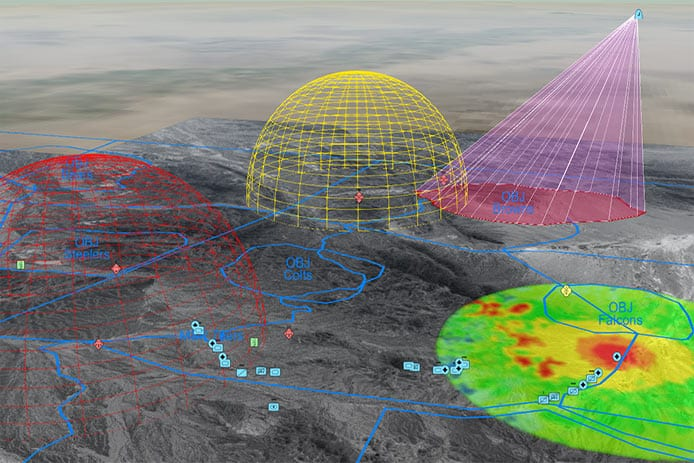
\includegraphics[width=2.5in]{fig/ewpmt.jpg}
\end{wrapfigure}
For other kinds of human-intensive studies, we will build a game where teams watch over a fleet of drones.
In that game, the screen will show a interactive topological map:
\bi 
\item    Markers will indicate locations  of   drones and humans.
\item Mousing on a region  will pop up   details on that region.
\item Mousing on drones will let humans     control the drones.
\item
Occasionally, little alert flags will pop-up pointing out potential pitfalls in the current situation. Each alert will come with a set of succinct questions offering suggestions on how to manage that alert,
plus one more option called ``other'' that will let operators do anything they like. Those alerts, including the suggestions,  will  be generated by our swarm optimizers running in the background, advising of events/decision that have  a high probability of making things better/worse. 
\ei
That interface will be iteratively improved based on evaluation from multiple stakeholders of various expertise (student novices and professionals) and genders. Co-PI Kuttal has created human-centric tools for developers using user-centered design and evaluation approaches.  
Previously, she has created tools that support programmer creativity \cite{Kuttal2020} and exploratory programming behavior \cite{Jernigan2017, Jernigan2015}, debugging web-based distributed programming \cite{KuttalSR13-chi, KuttalSBRKS19}, % REMOVED: KuttalSR13
problem-solving techniques \cite{Jernigan2017, Jernigan2015}, gender-specific behavior \cite{Kuttal2021g, Kuttal2019, Alexposter2022}, socio-technical skills \cite{Abimposter2022,Abimgitposter2022,Diwanjiposter2022,Zhou2018, sarma2016hiring, KuttalCWBS21, KuttalSRW18, abs-1810-13062} and communication styles \cite{Kuttal2020}.



 
\begin{table}[!t]
\caption{ In M-of-N studies,  a few $M$ humans monitor a large number of $N$ drones. }\label{mns}
{\small
\begin{tabular}{|p{.98\linewidth}|}\hline
\rowcolor{blue!10}
In an  {\em  m-of-n} study,  teams of $M$ humans will play a simulation game in which they must 
 monitor a fleet of   $N$ drones,   watching for off-nominal
situations, intervening when necessary.  \\
Just to give a flavor of the off-nominal problems our humans might be asked
to manage, here a few examples:
\bi
\item An emergency  team laying down a back burn must have a workable escape route.
Hence, if that team is working at one end of road and,   several miles away, a brush fire is encroaching   the escape route, then we must intervene to order the crews to down tools and rush their escape.
\item 
Drones in urban areas can fly up to 400' while Cessnas, monitoring those drones,
can fly down to 500'. In the case of approaching high winds, we must intervene to order the Cessnas to fly higher. \ei\\
\rowcolor{blue!10}
Note the monitoring challenge of the above two examples. Firstly, to see the problem, humans have to synthesize connections between
events occurring in remote parts of the simulation game.
Secondly, each drone in isolation could be working perfectly.
But when sets of drones co-ordinate with humans in a shared
space, some problems (like those above) become emergent.\\\hline
\end{tabular}}
\end{table}

\subsection{User Studies}
\noindent
Table~\ref{mns} discusses  the   ``m-of-n-studies''  used for our human-intensive studies. In these studies, a small number of human watch over a large number of drones looking for requirements violation.
\mbox{M-of-n studies}  are an excellent tool for controlled experimentation since they can  be run under a variety of well-controlled variations; e.g.
\bi
\item 
Decrease team size $M$; increase
number of drones being monitored $N$; 
\item 
Increase the number of problems introduced; 
\item 
Decrease the time available for solution etc.\ei 
% These times required to humans to detect, then respond, to requirements violations within the simulation
% can  be {\bf ablation studies} (see out text). \ITS{1} will be a success if the reaction times are faster and the proposed response is better when humans and AI work together to create those responses.
For the participants of such m-of-n studies, the challenge is staying alert   while   monitoring
all the information coming in from a large fleet of drones (visual images, sensor readings of the environment
inside and outside the drones, wind and weather reports, positions of humans on the ground, etc).
Faced with this information overload,
human operators often  become bored and fatigued and  distracted and   slow to recongize and react to new problems.  
 

 We conjecture that \IT~can address   operator fatigue.
 Rather than asking humans to watch all instruments reporting all features of model,
 we could ask instead for humans to engage with 
\IT.   \IT~ is a tool
 for ignoring most of the data and focusing instead on just a small region.
 We conjecture that by  
 tuning
the   frequency at which \IT~ interacts with humans, we think it possible
that can   engage the humans in some interesting, but not very taxing, problem
solving. If we tune correctly, then
these alerts will engage, not exhaust, the humans and so,  when novel and dangerous situations arise, humans
will quickly recognize and respond.

For further details on our user studies, see Table~\ref{studies}.




% All our studies   will cycle through two phases:
%  \bi 
%  \item For three cycles (run on different days):
%  \bi 
%  \item In the  \underline{\bf experience} phase, teams of participants   interact with the current requirements (with out without \ITS{1}) 
%  for a range of case studies for one to three hours. 
%  \item In the \underline{\bf debrief} phase, team members will debate why  they made different decisions about similar scenarios.
% We expect the debrief stage will lead to an update in the  requirements plus    updates to the control parameters of a model.
% A subsequent {\bf experience} phase will then test those updates.
% \ei
% \ei
% With the exception of some of the ablation studies (discussed below),
% \ITS{1} can be potentially beneficial  in both the {\bf experience} phase and {\bf   debrief} phase.
% During   the {\bf debrief}, \ITS{1} will help humans explore  trade-offs within a large space
%  of requirements.
%  Also, during the {\bf experience} phase, \ITS{1}  could    focus the human's attention on just the most important parts of the data

 


 

\begin{table}[!t]
\caption{Notes on our human-intensive studies.}\label{studies}
{\small
\begin{tabular}{|p{.98\linewidth}|}\hline 
\rowcolor{blue!10}
User studies will be conducted after the approval for
 NC State Investigator Review
Board (IRB). \\ 

We will match   user studies to the participant skills.
  Simple user studies (e.g. Amazon drones delivering packages to households, during
a thunderstorm) will be used for our work with NC State students.
On the other hand, 
the fmdtools models of \S\ref{egmodel} will be used in association with subject matter experts from the SMART-STEReO team. 
\\\rowcolor{blue!10}
Initially, we will work with teams of size $N=2$, then move to larger teams for years two and three.\\
Initially, we will run   simple user studies (e.g.a fleet of drones  delivering Amazon packages during a thunderstorm)
then  move to move complex studies. Finally, in year 3 we will explore  
{\bf case studies} based on the emergency response teams modeled in the fmdtool models generated
by the SMART-STEReO team.
\\\rowcolor{blue!10}
For our  initial small \underline{\em lab studies}
we will recruit university students. \\\rowcolor{blue!10}
For our \underline{\em case studies}, we will recruit  real-world subject matter
experts from the SMART-STERe team.
\\
 All our lab studies and case studies will explore models at various levels of ``stress''.
Stressing factors could be ``achieve more goals with fewer drones''; ``achieve more goals in less time'';
``achieve more goals with fewer team members'';
``achieve more goals in the presence of an increasing number of non-nominal scenariois'';
``achieve more goals when the time-to=failure of each drone becomes increasingly variable''.   \\\rowcolor{blue!10}
For data collection in these lab studies and case studies, we will:
\bi 
\item Initially use a
  think-aloud protocol \cite{lewisusing, Seaman1999} 
  where participants will   vocalize their thoughts and feelings as they perform their tasks.
  \item Conduct retrospective interviews to gain insights into participant experiences and barriers encountered during decision making with and without {\IT}.
  \item At the end, we will measure the cognitive load of the humans and usability of {\IT}. \ei \\
As in our past qualitative analyses (e.g., \cite{Kuttal2020, Kuttal2021g}), we will triangulate (compare and attempt to refute) the results with interviews and surveys to understand their strengths. %Retrospective interviews will be conducted to gain insights into participants' experiences and barriers encountered during decision-making with and without {\IT}. 
We will collect (1) Pre-surveys with standard questionnaires to collect demographics and familiarity with the domain of the model. (2) Pre- and post-surveys with standard questionnaires will be used to evaluate self-efficacy. (3)  User Experience Questionnaire (UEQ)~\cite{rauschenberger2013efficient,schankin2022psychometric,schrepp2014applying} to evaluate the usability of  {\IT} interface. (4) Measure participant engagement with the {\IT} tool using the ISA engagement scale \cite{soane2012development}, which is based on the view that engagement comprises 'intellectual,' 'social,' and 'affective' dimensions. (5) Post-surveys will be used to analyze the cognitive load \cite{CognitiveLoad}(such as using NASA Task Load Index~\cite{hart2006nasa})  to measure and conduct a subjective mental workload (MWL) assessment. \\\hline
\end{tabular}}
\end{table}

% For starters, we need to implement the PSO and LLM extensions described above. In our experience, this will raise numerous   design questions about the relative metrics of some tactic versus another;
% e.g.
% \bi 
% \item 
% Currently \ITS{0} clusters over some synthesized dimension that is analogous to PCA; so
% should \ITS{1} do that, or employ some other clustering method?
% \item Peng et al.~\cite{peng2022godel} assert that mixing gold plus rusty quries is useful for building LLM training sets.
% But does that policy work in this domain?
% \ei 
% The merits of these different tactics will have to be assessed with respect to case studies with real models and real subject matter experts.


\subsection{Measurements}
{\noindent}Table~\ref{metrics} shows the   independent and dependent variables to be collected as part of this study.  Most of these measures are self-explanatory; e.g. whatever we do with \IT~  and human-in-the-loop reasoning, we need to benchmark that against state-of-the-art fully automatic optimization tools such as FLASH, HYPEROPT and OPTUNA~\cite{bergstra2015hyperopt,nair18,akiba2019optuna} (see Table~\ref{metrics}, bottom-right, ``{\em nonhuman y-metrics}'').

But there are two sets of metrics worthy of discussion. Recall from the above that stakeholders are assigned their own particles which move from some initial
position to some final position. By measuring the median difference in particles between different
stakeholders before and after inference, then we can report initial and final divergence in team 
 opinion (and {\em decreased} divergence would be {\em better}). This metric is shown bottom-right of Table~\ref{metrics}
 as ``Initial and final divergence''.

 Also of note is the ``{\em cognitive load on the humans}'' shown top-right. Within the  cognitive psychology literature,
 there is a standard   questionnaire~\cite{CognitiveLoad} to quantitatively gauge cognitive load.


 


% Note the requirements engineering aspects of these m-of-n studies:
% \bi 
% \item To recognize ``off-nominal'', team members must have a shared understanding of what requirements need to be followed.
% \item To ``intervene when necessary'', team members must understand the capabilities of their tools such that they know what to adjust to repair   off-nominal events.
% \ei 


 

%%%%Recall from the above that stakeholders are assigned their own particles which move from some initial
% position to some final position. By measuring the median difference in particles between different
% stakeholders before and after inference, then we can report initial and final divergence in stakeholder
% opinion.
 


% in some analogue of PCA
% One factor that greatly simplifies all this experiemtnal work 

% Initially, small \underline{\em lab studies} will be conducted to understand developers' decisions in controlled environments. We will work with teams of size $N=1$, then move to larger teams for years two and three.

% After these smaller scale lab studies will come much larger scale
% \underline{\em case studies}.  For our \underline{\em lab studies}
% we will use university students   and for our \underline{\em case studies}, we will
% use teams use participants from the teams writing the models of \S\ref{egmodel}.
% Note that Co-PI Kuttal is  particularly skilled   with such lab studies and case studies (e.g., ~\cite{Kuttal2019, Lott2021}).

 
% \begin{wraptable}{r}{2.25in}
% \footnotesize
% \centering
% \caption{i* Models from~\cite{mathew2017shorter}.}
% \begin{tabular}{r|rr }
%  \textbf{Model} & \textbf{Nodes} & \textbf{Edges}     \\ \hline
% Services, see Figure~\ref{fig:scrumModel}.  & 351 & 510    \\
% Counselling & 350 & 470    \\
% Marketing & 326 & 422   \\
% Management & 206 & 239    \\
% ITDepartment & 126 & 162    \\
% Kids\&Youth & 81 & 81      \\
% IT Modernization & 53 & 57    \\
% \end{tabular}
% \label{tab:sizes}
% \end{wraptable}
%  \underline{\bf TASKS:}
%  As stated in the introduction,
%  we will run three studies. 
% A common feature 


% To avoid those problems, \ITS{1} will simulate models
% of the  emergency services' requirements. 
% In {\em CPU-intensive studies},  \ITS{1} will explore the requirements to find the most interesting/dangerous regions of the problems space. 
% Also, in {\em human-intensive studies}, we will see how early humans can detect and repair off-nominal drone behavior.  Humans will be asked to play a simulation game where they must monitor a fleet of   drones,  intervening when necesary. Unbeknownst to them, the game will  enact the   danger
% scenarios found in the CPU-intensive studies. 
% The \ITS{1} human-in-loop optimizer will be judged a success if, in the CPU-studies, it can quickly find the most interesting/dangerous scenarios. Further, in the human-intensive studies, success means that \ITS{1}'s questions   keeps the stakeholder engaged (but not exhausted) such that,  when danger scenarios creep in, they can quickly detect and mitigate them.

% Further, to test the above conjecture, we would then run an {\em ablation study} where the danger scenarios must be handled by (1)~the AIs  without human input or
% (2)~the humans without AI input.

 
% Our experiments will focus on \underline{\em serial  RE discussions} where some design artifact (the model) is being passed along a circle of stakeholders who may update the model before passing it down the circle
% (stopping when the model
% traverses the entire circle
% without revisions or comments).


% (Aside: For future work, we will explore ``parallel RE design discussions'' where N people
% debate the same version of a model at the same time (e.g. at some meeting). In justification of this focus on serial distributions, we note that this is a natural model for geographically remote workers who usually work on by themselves, sometimes interrupted by messages, emails, or status meetings with their manager.)


% In this work, we will also   explore gender issues leading to biases   using GenderMag \cite{Guizani, Chatterjee}, to  find and fix gender-related issues in problem-solving   and increase gender inclusiveness. 



 % \underline{\bf   INTERFACE:}
 % To begin with, our bot will offer a very simple text interface, sometimes with a question "rank the following
 % two options".  
% Initially, we will offer our participants
% a DISCORD channel to handle (and record) design discussions
% plus a 
% a simple directed-graph editor (with a search bar) to view our models. Edits to the model will be saved as pull-requests within Github (thereby offering a record of all revisions to model, tagged with the name of the person proposing a change.


% The final version or deployment version will be provided with a more sophisticated interface that allows explaining the decisions of the ADVICE. Further, it will also give suggestions based on the
% electrong footpring and teams during the decision-making process of stakeholders. The explanation and suggestions  will follow Shneiderman's guidelines \cite{Shneiderman1982} and Neilsen's heuristics  \cite{Nielsen1990}. 

%  \underline{\bf   CASE STUDY MATERIAL:}
% The first step in the workflow is to gather the requirements con-ops documents from different emergency response teams, then build their associated fmdTools models. This first step has been underway now for two years and this proposal will take advantage of that work product. 

% Next we will script up the environment that can run the fmdTools models, and display their results. Some visuals will be added to observes can imagine that this data is collected from  
 
%  After that, we will have meetings with the SMART-STEReO team to identify some useful scenarios (perhaps, even, looking at their historical logs to see what kinds of simulation results lead to most changes
%  to their models). 
%  The scoped studies will then be sorted by ``domain knowledge needed to monitor the drones''.
%  If the domain knowledge is something simple like ``do not run out of fuel'' or ``do not exceed this threshold for max acceleration'', the scenarios are suitable candidates form our studies with NC State students. And if the required domain knowledge is complex such as ``implement standard operating procedures for firefighters in a class7 smoke-field envrionment'', then that scenarios would be slated for running with volunteers from the SMART-STEReO team.

% At that point we can start the CPU-intensive studies to find the most severe problems with the current requirements.  Once found, we would cache those problem scenarios (for use in the human-intensive studies) before asking the CPU-intensive studies
% to search for mitigations to those problems.

% Once we have some interesting problems, we can start the human-intensive studies.

 
 

%   \underline{\bf CASE STUDY MATERIAL:} Year1 (with NC State students) will use 
% relatively simple models taken from the SE research literature (e.g. the product line of Figure~\ref{fig:scrumModel}. Then, to stress test our ideas,  we would take advantage of the flurry activity around the SMART-STEReO group building the \S\ref{egmodel}'s models. As mentioned above, this is a very active and well-funded group doing much current work.  We would watch that activity, find decisions are made based on simulation output, and then \underline{{\bf replay those decisions}} with our tools (to see if a different and better conclusion might be reached, using less simulation time). 
  
% \underline{{\bf Replaying those decisions}}  will not be an onerous task.
% Firstly,  the SMART-STEReO group has an established procedure for sharing models.   In the COVID era, to enable remote work on that project,
% this group created policies by which they can build laptop software with all the licenses and permissions needed to work securely on these materials. Now it is routine for that group
% to have interns working on those models, from around the country, logging-in via those secure laptops.

% Secondly, repeating a simulation study is often a daunting task, since it requires the CPU farms needed for the original study. But recall that {\ITS{1}} uses
% {\ITS{1}} recursive bi-clustering procedure, evaluating only 2 examples at each level of the recursion\footnote{Formally, this makes {\ITS{0}} akin to the SIMPLEX method~\cite{muller1979location} that finds vertices
% of a system of linear inequalities,  then favors samples of those points (since they
% are most informative). \ITS{0}  searches through some data points that fall within some multi-dimensional polyhedron. \ITS{0}'s search for distant points means that  it finds, then evaluates, the vertices of that polyhedron-- which is a non-parametric analogue to the  points sampled via   SIMPLEX. But note that we favor \ITS{0}'s method over SIMPLEX since the latter requires optimization problems expressed in some high-level equational form (whereas \ITS{0} can work
% from the log of the output of any model at all).}. In practice, this means that {\ITS{0}} (and hence {\ITS{1}}) should be able to replay
% conclusions from $N$ evaluations using just  $2\log_2{(N)}$ evaluations
% Better yet, we may not even have to rerun the simulations.
% With access to a log of all the evaluations made during the original study, we might be able to use some partial match approach to make do with similary, but not exact, old rows for our new queries.


  

 

%This workflow will  make it convenient to conduct large scale studies where we invite (say) 1000s of industrial practitioners (via email) in order to attract 100s of participants.






%   Some of our research questions (see below) require us to run numerous large teams.  For that purpose,
% we will use Mechanical Turk (MTurk) to recruit  large sets of participants (>300). MTurk is used extensively by academics as a quick and cheap means of collecting questionnaire data, including software engineering research, from a diverse sample of participants.  E.g. Stolee used "Turkers"   look for bugs in regular expressions~\cite{stolee2010exploring} while Stolee and Menzies
% used "Turkers"  to comment on Github pull requests~\cite{chen2019replication}.
% When using MTurk it is important to 
%   augment any pre-screening with "gold tasks"
% which are a small number of work packets with known results that are slipped into
% the "Turkers" workflow. By pruning "Turkers"
% who fail on the gold tasks,  Stolee and co-PI Menzies found   that at least  50\% of
% their workers has sufficient skills relevant for details SE design and implementation tasks.

% Initially, we will   balance gender and race since prior studies warn that  such balance  is crucial to prevent algorithms from perpetuating social inequities~\cite{Leavy2018}.
% Later,  when \ITS{4}   explore issues of bias and discrimination, we will use teams with a   variety of diversities.
%  We will conduct multiple lab studies to bolster confidence in the results. To allow more gender and expert diversity we will conduct virtual lab studies.  Virtual lab studies will recruit participants via snowball sampling, ads on social platforms, and recruitment websites such as Upwork.



 


% Furthermore, since the literature \cite{Kuttal2019, Lott2021} indicates gender differences in communication, more comprehensive gender-inclusive language  \cite{festante2007, miller2001handbook} is needed to prepare suggestions to engage, provide non-authoritative suggestions \cite{Seymour2017}. In order to generate accurate suggestions, we may need to consider cues from both study participants as well as cloud. 

 % \underline{\bf METHODOLOGY:} 

 % XXX? i
 
% For data collection,
% the think-aloud method \cite{lewisusing, Seaman1999} will be used. Participants will   vocalize their thoughts and feelings as they perform their tasks.   Participants in a control group will perform tasks using appropriate state-of-the-art optimizers suitable for comparison with automated version of {\IT}. Based on our literature review~\cite{lustosa21} (as of 2021) FLASH and HYPEROPT and OPTUNA~\cite{bergstra2015hyperopt,nair18,akiba2019optuna} will be utilized
% (we will update those comparison
% tools to reflect the ongoing state-of-the-art).

% As in our past qualitative analyses (e.g., \cite{Kuttal2020, Kuttal2021g}), we will triangulate (compare and attempt to refute) the results with interviews and surveys to understand their strengths. Retrospective interviews will be conducted to gain insights into participants' experiences and barriers encountered during decision-making with and without {\IT}. We will collect (1) Pre-surveys with standard questionnaires to collect demographics and familiarity with the domain of the model. (2) Pre- and post-surveys with standard questionnaires will be used to evaluate self-efficacy. (3) Post-surveys will be used to analyze the cognitive load using NASA Task Load Index~\cite{hart2006nasa}  to measure and conduct a subjective mental workload (MWL) assessment. 
 

 
%  \underline{\bf DATA ANALYSIS:} Our specific research questions require the collection of specific metrics:
% \bi
% %  Video data, audio data, and screen interactions of developers will be collected as transcripts, which will be analyzed using a mix of qualitative and quantitative measures. Qualitative methods from Grounded Theory \cite{GlaStr67} (e.g., Corbin and Strauss variant \cite{strauss1990basics}) will be used to analyze the transcripts.  We will annotate points based on developer utterances to identify key concepts and phenomena via an iterative, open-coding process, especially for artifacts or experience-based cues when making decisions.  This process will also be used to analyze decision-making behavior.   Finally, thematic analysis \cite{Braun2006} will be used to organize qualitative data into themes that relate back to the research questions.  Non-parametric effect size and significance tests   will be used for quantitative analysis.
% % Further to the above, some of 
% \item
% \underline{\em Stakeholder category metrics :} One goal of this work is to better support model-based reasoning for different categories.
% Under some anonymization   protocol, {\em participant diversity} will be collected
% (with categories such as age, gender, racial background, veteran status, accessible challenges, etc.)
 
% % \underline{\em Bias Metrics:} Our bias mitigation metrics
% % were discussed in \S\ref{bias}. Note that we would ensure we can report  these metrics separately
% % for all different stakeholder categories.
% \item
% \underline{\em Initial and final divergence metrics:} For   teams of size $N>1$, we   use PSO to measure initial and final divergence before and after   inference 
% (and, ideally, that difference decreases from initial to final).
% Recall  from the above that   stakeholders
% are assigned their own particles which
% move from some initial position to some final position. By measuring the median difference 
%  in particles between different stakeholders before and after inference, then we can report   
%  initial  and   final
%  divergence  in stakeholder opinion.
% \item
% \underline{\em   $y$ metrics:} Stakeholders  often explore
% multiple goals, where the $y$ goals might be contradictory. We need some trade-off predicate
% that knows how to report improvements on multiple dimensions. We will use the
% Equation\ref{eq:cdom}  calculation
% from Table~\ref{advice1}. As mentioned above,  this calculation is  preferred to  standard ``boolean domination'' (one thing is better than another if it is no worse on any criteria and better on at least one criterion), since it is known that boolean domination can  fail for three or more goals~\cite{Wagner:2007, Sayyad:2013}.
% \item
%  \underline{\em Acceptance  metrics:}    $y$ metrics    only comment on terms     in a model. Above and beyond that, we need    our post-surveys to capture   other concerns from stakeholders   about the acceptability of our final models.
%  \item
% \underline{\em  Nonhuman-$y$ metrics:}
% To calibrate and baseline the {\IT} $y$-metrics, we collect output $y$ values
% seen in     AI tools that make all the decisions themselves, with no human involvement
% (e.g. 
% FLASH, HYPEROPT and OPTUNA~\cite{bergstra2015hyperopt,nair18,akiba2019optuna}).
% \ei
% % \textbf{Methodology} Each student will complete decision task using the think-aloud method. They will record their decision making sessions. We will conduct surveys on their experiences, knowledge tests and end-of-term student course evaluations. Each professional will complete decision based HIT (Human Intelligence Task) using MTurk followed by surveys on their experiences with CROWDED. HIT will have attention checks. An attention check is a question designed to verify that the respondent is reading questions and responding with care. 


%  \underline{\bf ABLATION STUDIES:} 
% % \textbf{Data Analysis} Quantitative measures (such as ANOVA) will be used to analyze the scores on tasks, and self-reported surveys on decision making experiences. 


\section{ Research     Plan}\label{rqplan}
For full details of our research plan,  see  the {\em Collaboration Plan} supplemental document. In summary:
\bi 
\item In all years, NC State will be a frequent visitor to the SMART-STEReO team (in California).
All user studies will be designed with subject matter input from that site.
\item 
Also, in year1, NC State will build {\IT}, version 0.1 and gaming interface. 
\item 
Year2, will have  some initial, and limited,   interaction between subject matter experts and our tools.
\item
In year3, much data will be collected from a very large number of user studies, many of which will include studies with participants from the  SMART-STEReO  team.\ei
Also, in all years, we will explore  {\em  broadening participation in computing}.
One  of the benefits of  NSF funding is the opportunity to work on  broadening participating in computing (BPC).  Our BPC plans are discussed in \S\ref{bpc}.  BPC will be an ongoing task through-out the work.

%Table~\ref{tbl:plan} shows some planned milestones for this research work. 


\begin{table}[!t]
\caption{Metrics for this Study.}\label{metrics}
{\small \noindent\begin{tabular}{|R{.12\linewidth}|R{.34\linewidth}|R{.48\linewidth}|}\hline
 \rowcolor{blue!10} Notes & Independent variables  & Dependent  variables  \\\hline
Human-level measures & 
\bi 
\item Demographics about teams: size of teams; years of experience with each other; etc. 
 \item 
 Demographics about individuals: age, gender, racial background, veteran status, accessible challenges, years of experience with the case study being used; etc.
\ei
&
\bi 
\item Time to recognize a requirements violation in the simulation;
\item Time to resolve that violation;
\item Number of delayed actions per minute;
\item  Number of forgotten  actions per minute;
\item Number of interrupted actions per minute;
\item Average interruption time (seconds per minutes)
 \item Cognitive load on the human. \ei\\
 \rowcolor{blue!10}  Domain-specific measures 
 (different case studies may have    different domain-specific success
criteria). & 
For example:
\bi 
\item 
Types and size (number of words) of electronic footprint available  per team member.
\item 
Size of requirements models; e.g. number of variables; number of constraints; 
average constraints per variable; etc.
\item Nature of the goal space; e.g. how many objectives; how many objectives are conflicting; etc. 
\ei & For example:
\bi 
\item When delivering packages for Amazon, the goal might be 
{\em most} packages delivered in {\em least} time by {\em fewest} drones.
\item for emergency response groups fighting  a brush fire,
the goals might be 
{\em minimize} the property damage  during  simulation of a brush fire while
also 
{\em minimizing } the lives lost or injured during the simulation of the brush fire. \ei\\
Domain-general measures 
(these should apply to most case studies)
& Amount of ``stress'' in the simulation. Recall {\em m-of-n} studies
can be stressed in various ways such as decreasing the number of $N$ humans,
increasing the number of $N$ drones; decreasing the required response time; increasing the number of
problems injected into a simulation.
&
The following are goals for the multi-objective simulation.
\bi 
\item {\em  Minimizing} acceleration stress on the drone rotors ;
\item {\em Maximize}   battery reserves when drones return to base;

\item 
{\em Acceptance metrics}:Using
post-surveys,  capture   concerns from stakeholders about the acceptability of our final models.
\item 
{\em Nonhuman-y metrics}: To calibrate and baseline the ADVICE y-metrics, we collect output y values seen
in AI tools that make all the decisions themselves, with no human involvement (e.g. FLASH, HYPEROPT and OPTUNA~\cite{bergstra2015hyperopt,nair18,akiba2019optuna});
\item {\em Initial and final divergence metrics}:   Looking at PSO particles,
measure  
divergence between team members before and after inference (ideally,   difference decreases from initial to final).
\ei\\\hline
\end{tabular}}
\end{table}


%\newpage
 \section{ Research Questions}\label{quest}

 

% Please add the following required packages to your document preamble:
% \newcommand{\X}{\ding{52}}
% \begin{table}[!t]
% \caption{Research Plan.}\label{tbl:plan}
% \footnotesize
% \begin{center}
% \begin{tabular}{lp{5in}|l|l|l}
% Task && Y1 & Y2 & Y3 \\\hline
%  Setup & Build a baseline implementation of \ITS{1}, version 0.1  & \X & \\
%  Bot   & Build   baseline versions of the interface & \X & &\\
%  RQ0&   Do people and \ITS{} find different solutions for completing design tasks?    & \X & \X & \X \\
% RQ1&   Do humans using \ITS{} perform better than (a) humans, fully manually  (b) AND   AI tools   humans? & \X & \X & \X \\
% RQ2 & How to select terms for prompt engineering? & \X & \X & \\
% RQ3&   For \ITS{1}, how to weigh PSO’s cognitive versus social reasoning?                &   & \X &   \\
% RQ4&   Is  \ITS{1},’s team support “useful”?                                              &   & \X &   \\
% RQ5&   Is there a max “team size” threshold above which \ITS{1} would not be recommended? &   & \X &   \\
% RQ6&   Are different kinds of background knowledge most useful for \ITS{2}?                    &   & \X &   \\
% RQ7&   Do different categories of stakeholders need different support for their different cognitive styles?                                      &   &   & \X   \\
% RQ8&   (if time permits) Can {\IT} support test case generation?                                          &   &   & \X\\ 
% RQ9&  (if time permits)   Can {\IT} guide the creation of the model?                                          &   &   & \X\\\hline
%  Also   & Work on BPC (broadening participation in computing).                           & \X & \X & \X  
% \end{tabular}
% \end{center}
% \end{table}


\subsection{{\bf CPU-Intensive} Questions} These research questions will focus on the measuring and then improving the algorithmic performance of \IT.

{\bf RQ1 (Year 2)  {\em For \IT, how should we weight PSO's cognitive versus social reasoning?} }
   Recall that PSO determines the new velocity of a particle from the sum of a personnel's cognitive weight
    $\phi_p$ and the group social weight  $\phi_g$.
    The specific values for these weights in this work will be determined through experimentation, potentially learned via a self-adaptive scheme~\cite{harrison2018self}
or through configuration hyperparameter optimization~\cite{8469102}). Initially, we consider the advice from Pedersen~\cite{pedersen2010good}, who recommend  $\phi_p+\phi_g \approx 4$ (bearing in mind that distance weights are normalized between 0 and 1). 
\underline{ Relevant metrics:} The vpttrvy $\phi_p+\phi_g$ optimizes for both the 
  y-metrics and
the acceptance metrics of   Table~\ref{metrics}, bottom-right.
% \end{description}
% \vspace{-10mm}
% \begin{description}


{\bf RQ2: (Year 1,2) {\em How do we choose terms for prompt engineering?}} Recall that researchers in large language models (LLM), such as Peng et al.~\cite{peng2022godel}, emphasize the importance of carefully selecting training words for LLM prompt engineering. As discussed in Section \ref{cloud}, Peng et al. recommend achieving an equal balance of terms with the highest and lowest language model (LM) loss. While this recommendation was valuable in their domain, in the context of our research questions, we will conduct experiments with term selection.
 %Recall that LLM researchers like Peng et al.~\cite{peng2022godel} recommend the careful selection of training words for LLM prompt engineering. As discussed in \S\ref{cloud}, Peng et al. recommend an equal balance of terms  with  highest and lowest LM loss. That was useful in this domain but in this resaerch questions,  we would experiment with term selection. 
  \underline{Relevant metrics:} The right term selection results optimizes for  
the acceptance metrics (see Table~\ref{metrics}, bottom-right). 

\subsection{{Human-Intensive} Questions}
In addition to qualitative measurements obtained through the Think-Aloud Protocol, which involves having users verbalize their thoughts and experiences during interaction to provide insights into usability, engagement, and cognitive load, we will employ behavioral observations. Behavioral observations entail observing user behavior, hesitation, and decision-making patterns during tasks. To complement these qualitative methods, quantitative measurements will be applied to address following RQs focused on the overall performance and usability of the \IT~tool.

{\bf RQ3: (Year 1,2,3) {\em What are the key usability factors of the \IT~tool, and how do they impact user experience for first responders?}}
In controlled settings, we will assess the usability and engagement of the \IT~Tool with and without it. Additionally, we will conduct comparisons with earlier versions of the \IT~Tool to ensure continual improvement in usability and engagement with each iteration.
\underline{Relevant metrics:} UEQ responses, IST scale responses, Time to recognize a requirements violation in the simulation; Time to resolve that violation; Number of delayed actions per minute; Number of forgotten  actions per minute; Number of interrupted actions per minute; Average interruption time (seconds per minutes).

{\bf RQ4: (Year 1,2,3) {\em Does the \IT~tool help decrease cognitive load?}}
After each task performed by participants, we will measure   aspects of workload, including mental/  physical/  temporal demand, performance, effort, and frustration.
\underline{Relevant metrics:} NASA Task Load Index responses. 

{\bf RQ5: (Year 3)  {\em Do different categories of stakeholders need different support for their different cognitive styles?}}
    For this RQ, we   check
    if our tools need different styles of interfaces.
    Prior results
    from co-PI Kuttal 
    shows that different categories of stakeholders can have different decision-making styles~\cite{Kuttal2019}
    (for example, women participants perceived constructive feedback from another woman while men participants perceived hurtful feedback from another man). If so, then this would have two consequences. Firstly,
    it might mean we should engineer different model browsing environments for different categories of stakeholders. Secondly, those different styles might suggest better algorithms for the internals of our search.   
  \underline{ Relevant metrics:} All the RQ2 metrics, divided according to our Stakeholder category metrics. 

\subsection{Questions about Ablation Studies}
In this research questions, we check if any parts of our design an over-elaboration. To to this, we re-run all the above experiment after removing some part of the system. 


{\bf RQ6: (Year 1, 2, 3) \emph{Do users employing {\IT} achieve better results compared to (a) humans working entirely manually {\bf AND} (b) running AI tools without human-in-the-loop?}}
This serves as baseline prudence check. If RQ6=no, it would imply that AI+human performs worse than applying either separately. Current results ~\cite{lustosa21,lustosa22} with {\IT{0}} suggest RQ6=yes, but, as mentioned above, this needs validation for each new model explored by the system.
\underline{Relevant metrics:} 
From y-metrics, the acceptance metrics, and the nonhuman y-metrics. 
 
 %{\bf  RQ6: (Year 1,2,3) {\em Do people and {\IT} find different solutions for completing design tasks?}  }
%  This is one of our baseline prudence checks. %If  RQ0=no, then all this work is a waste of time.
%Based on our current experience with \ITS{0}~\cite{lustosa21,lustosa22}, it would seem that RQ1=yes. This should be checked on each new model explored by this system.
% \end{description}
% \vspace{-10mm}
% \begin{description}

{\bf RQ7: (Year 2) \emph{Is {\IT}'s team support "useful"?}}
\underline{Relevant metrics:} Does \IT~ enable humans to achieve a task (e.g., optimization) with lower cognitive load and "good" results (i.e., high $y$-value scores)? Are these results acceptable to the team (measured using divergence scores)?

{\bf RQ8: (Year 2) \emph{Are different kinds of knowledge most useful for \IT?}}
Table~\ref{info} lists a wide variety of cloud knowledge sources. In practice, only some (or none) of them might be accessible or useful. To answer this RQ, we will experiment with different cloud knowledge sources and compare the results of \IT{2} to \IT{1} using the same metrics as RQ7.
\underline{Relevant metrics:} Same as RQ7.

{\bf RQ9: (Year 2) \emph{Is there a maximum "team size" threshold above which {\IT} would \textit{not} be recommended?}}
Here, we investigate a potential confounding factor in the above results. We suspect that our methods will work up to some threshold "max team size," and beyond that, there might be a breakdown. We aim to confirm this through experimentation.
\underline{Relevant metrics:} (Size of team) versus (y-metrics, acceptance metrics, task completion time).


% \end{description}


 

% % \begin{description}
%   \item[RQ7:] (Year 3)  {\em  For \ITS{3} Can   meta-patterns of advice support  verification?}
%     \hfill \\  
%       \S\ref{verify} discussed how advice ``patterns''
%       of  (a)~how often it is revised and (b)~how that advice
%       effects our ability to  predict progress in the design process, and (c) other patterns.% as well and several others. 
%       This RQ will check if  we can find those patterns and if we can use them
%       to  select better advice,
%       or mitigate for bad advice. 
%     \\
%   {\bf Relevant metrics:}    Same as RQ3. 
% %   \end{description}

% % \begin{description}
%   \item[RQ8:] (Year 3)  {\em  Are {\IT}'s models biased againt specific social groups?}
%     \hfill \\  
%       Before we explore bias mitigation (in the next RQ), first we must check if
%       our models exhibit bias.
%     \\
%   {\bf Relevant metrics:}    There are  at least two ways to detect bias in a model: (1)~use the bias measures of
%       \S\ref{bias} ; (2)~check the post-surveys for any bias-related concerns (as reported
%       by our participants).
% %  \end{description}
 

% % \begin{description}
%   \item[RQ9:] (Year 3)  {\em  How does \ITS{4} effect model bias (if at all)?}
%     \hfill \\  
%       \S\ref{bias} discussed methods for model bias  mitigation
%       including personnel balancing, extra
% context, hyperparameter optimization, and sample balancing. (Aside:   recall
% that ``extra context'' really means dialing up, or down, how much information we import from
% Table~\ref{info}.).  Here we would deploy teams with various degrees of diversity (as
% measured by our stakeholder category metrics). Those teams would be supported by different
% combinations of extra
% context, hyperparameter optimization and sample balancing. Note that this would be a very
% large set of case studies.
%     \\
%   {\bf Relevant metrics:}   Same as RQ8. 
% %  \end{description}

 
% % \begin{description}
%   \item[RQ10:] (Year 3)  {\em With \ITS{4}, does mitigating bias mean damaging performance?}
%     \hfill \\  
%      Recall the concern raised above   by  Berk et al.~\cite{berk2017fairness}   who said
% ``It is impossible to achieve fairness and high performance simultaneously (except in trivial cases''. At FSE'21, PI Menzies and his student Joymallya Chakraborty found that Berk et al. were needlessly pessimistic, e.g., sample balancing to mitigate bias while preserving  predictive performance.
% But that result was only for classification systems. In this RQ, we need to check if bias
% mitigation damages performance in multi-goal optimization. Note that if we see such
% damage, then it might be repairable (by extending the hyperparameter optimization methods
% of \S\ref{bias} to explore not just bias metrics, but $y$ value performance metrics as well.
%     \\
%   {\bf Relevant metrics:}   Same as RQ3, plus the bias metrics.  
% %  \end{description}
 
% \begin{description}
%{\bf RQ8:}   (Year 3)  {\em  Can {\IT} support test case generation?}  (  if time permits)
 % At its core, {\IT} explores a design looking for settings that most  select for different behaviors. If we turn off user input and  ran {\IT} $N$ times with different random number seeds, then that would generate a set of vectors that separate the data into its most critical regions. This is clearly a way to generate tests
     %that are spread across the input space of a model.  In this RQ we would conduct a literature review to (a)~document the current state-of-the-art (SOTA) in model-based test generation, and (b)~discover what is current thinking on how to evaluate test coverage.  We would then apply those coverage metrics to tests generated by {\IT} or SOTA.  {\bf Relevant metrics:}  Test coverage metrics, as documented by the  literature review of this RQ.

%{\bf RQ9:}  (Year 3)  {\em  Can {\IT} guide    the creation of the model? }  (  if time permits) So far in this proposal we have assumed that we are checking models created by the SMART-STEReO group. It has not escaped our attention that   our tools could also  authoring of models. Recall that the  SMART-STEReO   builds   models from ConOPs (concept of operations) docs written by the different emergency services. Given the ConOPs test, and the   preference knowledge in our  LLMs,  it should be possible to guide the model creation process towards the issues of greatest current interest.  {\bf Relevant metrics:}  Time to generate a model,  coverage metrics, as documented by the  literature review of this RQ. All the RQ2 metrics collected on the models. where mode creation is guided by the LLMs.

  
 


  
% \ei
% \subsection{Models Evaluations timm(prune, cull)}
% We will explore different designs for an iSBSE with the goal of let a \underline{\bf broad}
% participants explore \underline{\bf many} models to find \underline{\bf better} solutions with \underline{\bf least} effort that are more \underline{\bf acceptable} to more developers. 

% We will compare the performance of many models across to increase the generalizability of CROWDED.
%  In our prior work assessing SBSE and iSBSE algorithms~\cite{lustosa21,lustosa22,nair18,Nair2016,jchen19} we have found ready access to  10+ models per paper (on effort estimation, agile project planning, waterfall project planning, various configuration models, etc.) to evaluate our methods. More than that, another way to explore many models is to take an existing model and to mutate it such its size increases (measured in terms of number of nodes),  or its complexity increases (measured in terms of number of constraints per node) or both. We have used such model mutators in prior research~\cite{lustosa21}.
 











% \begin{figure*}[t]
% \centerline{\includegraphics[width=0.98\textwidth]{fig/PLAN.PNG}}
% \caption{3-year plan. Initially our
% interface will be very simple (same as Fig6) bit as we learn more about the decision making styles needs of different classes of stakeholder's we will adjust our interface tools to give the explorations methods that suite their style.}
% \label{Overall}
% \end{figure*}


% \section{Overall Plan and Schedule}
% The proposed research will involve laboratory studies, interviews, surveys and case studies.  The continuous data collection, evaluation and refinement cycle will incrementally evolve ADVICE functionality. Figure \ref{Overall} shows the phased research plan over the three-year project period. 

% Efforts in Year 1 will focus on collecting Cues related to cognitive and social weights for ADVICE1-4 using ADVICE0. We will conduct gender and expert-balanced lab studies to collect initial set of cues utilized by the stakeholders when making decisions. Remember cues are the social and cognitive weights of the model that helps to prioritize the decision from different stakeholders. Further, to increase the reliability of the cues we will conduct case studies with students in SE classes and  professionals on Mturk. The tasks designed will help collect the respective cues as well as strategies when make decisions by stakeholders. Later, we will increase our confidence in the cues collected using lab study, case studies, and literature reviews by creating a large scale survey, followed by interviews. Towards end of Year1, the focus will be to develop ADVICE1 model that utilizes the expert's experience based cues and will be evaluated using model. RQ1 will be explored and user studies will measure: (i) higher accuracy of the model, and (ii) specific negation cliffs for the model weights. 

% In Year 2 the focus will be to develop ADVICE2 that utilizes cloud based cues (automatically generated from logs as in Table 2). We will evaluate the model with different weights to evaluate the best weight distribution strategy used by ADVICE2. Based on the finalized model we will use a simple interface to evaluate the model with gender and expert-balanced lab studies as well as case studies. We will collect qualitative and quantitative data.  Qualitative analyses will focus on transcripts and interviews; this will help also collect the decision style of different stakeholders. Quantitative analyses will employ the Wilcoxon rank-sum test or t-tests. The metrics include: (i) student and professional task success; (ii) completion times, (iii) student experiences (e.g., satisfaction and engagement) with ADVICE2 using end-of-term student course evaluations, (iv) accuracy of questionnare score with the model score. 

% Towards second half of Year2, ADVICE3 will be developed with verification support and will be evaluated by comparing various fixing techniques from literature for specific conflicts. ADVICE3 will be improved with better interface that generate feedback as well as explanations for ADVICE3 advice and decisions. ADVICE3 will evaluated using Comparative case studies with students and professionals. In class settings students will complete (i) first assignment without ADVICE3; (ii) second assignment with ADVICE3; and (iii) third assignment optionally with ADVICE3.  Similarly, using Mturk participants will complete decision making tasks with and without ADVICE3. Three-way ANOVA and two-way between-subjects tests will be used to measure decision performance and model acceptance. Further, the scores (from the model) will be compared to participants questionnaires. The results will also help assess the usability and generalizability of ADVICE3 in real-world settings. Additional metrics for model evaluation: Based on what we have seen in traditional software analytics, there are two expectations. (i) frequency of the Faulty advice, and (ii) time to fix faults (should have some exponential decay where most are fixed quickly, but a few may take comparatively much longer). We will explore RQ1-RQ6.

% In year3, we will develop ADVICE4, whose interface design will be inspired from gender-based research and evaluated with GenderMag (as discussed in Section XX). Further, the model will be improved to minimize social biases by including related measures in the PSO optimization goals.  Based on the finalized model we will evaluate ADVICE4 with gender and expert-balanced lab studies. We will collect qualitative and quantitative data.  Qualitative analyses will focus on transcripts and interviews. Quantitative analyses will employ the Wilcoxon rank-sum test or t-tests. Additional metrics: (i) gender-based biases, (ii) highest model accuracy with bias-based metrics. 

% The final version of ADVICE4 will be evaluated using case studies in the classes and using Mturk. We will collect the data from different race and gender especially in our MTurk studies.We will explore RQ1,R7-RQ11. 

%  A unique aspect of this project is that the research efforts will continuously advance educational initiatives that will constantly steer research activities to ensure that the results are robust, effective and practical.   During end of Year 3, the ADVICE prototype will also be disseminated to obtain feedback to continuously refining the prototype. ADVICE will support industry methods to advance decision making and, of course, increasing diversity in computer science .

% Lastly,  one  of the benefits of  NSF funding is the opportunity to work on  broadening participating in computing (BPC).  Our BPC plans are discussed in \S\ref{bpc}. As seen in our timetable, BPC will be an on-going task through-out the work.
  \section{Intellectual Merit and Broader Impact}
  

\subsection{Intellectual Merit}

%This research explores uncharted territories in SE, introducing innovative methodologies to address inference in the midst of team disputes. It distinguishes itself by prioritizing collective team decision-making and seamlessly integrating symbolic and sub-symbolic models, providing a multidimensional approach not present in current research paradigms. The transformative nature of this research promises to revolutionize decision-making in software design.
This research introduces methodologies in SE to address inference challenges during team disputes, navigating uncharted domains. In response to the surge in AI-assisted tools, a key innovation lies in actively incorporating human feedback, prioritizing collective team decision-making, and seamlessly integrating symbolic and sub-symbolic models. This multidimensional approach sets it apart from current research paradigms. The intellectual merits of this work encompass: (1) Methodological Framework: The development of a robust methodology applicable to decision-making domains, offering advancements for fellow researchers in diverse fields. (2) Model Sharing: Dissemination of models and the {\IT} tool to the wider research and practitioner communities, fostering collaboration and enhancing capabilities in software engineering and decision-making. (3) Algorithmic Insights: Contribution of valuable algorithms, visualizations, and essential decision-making parameters and rules, providing a foundational resource for informed choices and effective problem-solving. (4) Empirical Insights: Each study conducted to enhance {\IT} generates empirical data and insights, enriching the scientific understanding of decision-makers in the domain. This research has the potential to revolutionize software design decision-making.






%This research delves into unexplored domains of SE, introducing innovative methodologies addressing inference amidst team disputes.  The study distinguishes itself by prioritizing collective team decision-making and seamlessly integrating symbolic and sub-symbolic models, offering a rich, multidimensional approach absent in current research paradigms. Its transformative nature promises to revolutionize software design decision-making

%This research aims ro encompass the creation of an innovative and practical tool, ADVICE, designed to facilitate decision-making for first responders. Additionally, we make the following research contributions: (1) Methodological Framework: We have developed a robust methodology that can be readily applied by fellow researchers in related decision making domains, facilitating advancements in their work. 
%(2) Model Sharing: We are sharing our models and the ADVICE tool with the wider research and practitioner communities, fostering collaboration and enhancing the capabilities of professionals in software engineering and decision making fields. 
%(3) Algorithmic Insights: Our research contributes valuable algorithms, visualizations, and essential decision-making parameters and rules, providing a solid foundation for informed choices and problem-solving
%(4) Empirical Insights: Each study conducted to improve ADVICE generates empirical data and insights that contribute to the scientific understanding of the domain of decision makers.

\subsection{Broader Impacts}

The project's broader impact is comprehensive, addressing five crucial areas. (1) It advances discovery and enhances education by reshaping the curriculum for graduate Software Engineering classes. Engaged students delve into interdisciplinary research at the crossroads of AI, SE, and HCI. Additionally, they gain valuable hands-on experience through internships at NASA, fostering collaboration and the development of lifelong professional relationships. (2) The project is committed to actively mentoring underrepresented groups, reflecting the significant contributions of both PIs to diversity and inclusion. Students involved in the project will have the opportunity to attend prestigious events such as the Grace Hopper conference and the Richard Tapia Celebration of Diversity in Computing. Additionally, a dedicated portion of the grant will be allocated to support initiatives focused on Broadening Participation in Computing (BPC). (3) The collaboration with NASA enhances infrastructure, providing access to extensive logs and field data. The team's diverse expertise ensures robustness. (4) Broad dissemination will be achieved through  through the publication of research in leading SE venues and sharing knowledge via keynotes and invited talks. Emphasizing open science, all project scripts, models, and data will be accessible on GitHub, freely available for researchers and industrial practitioners. (5) The work explores the synergy between humans and AI, introducing transformative concepts in decision-making with applications in security, safety, and software engineering, thereby carrying significant societal implication

Further, the team is well-qualified and diverse, with members possessing the expertise needed for this research -  PI specializes in building AI optimizers and Co-PI excels in studying human subjects and creating tools tailored to their needs. Dr. Misty Davies, affiliated with NASA Ames and an expert in building fmtool models, is also part of the SMART-STEReO project. 








% Bringing humans in the loop of the decision-making process for AI-based systems is an important area to explore in SE research. This could help to mold models better to human processes and potentially make them more explainable or interpretable.
 
 %Given the rapid rise of AI-assisted tools for developers, exploring work that more closely involves human-feedback will be an important line of work, and one that bears fruit for various SE tasks.



 


	% \section{PI's strengths}
	
	% The proposed research will draw on Dr. Kuttal's experience creating human-centric tools for developers using user-centered design and evaluation approaches.  She have created tools that support programmer creativity \cite{Kuttal2020} and exploratory programming behavior \cite{Jernigan2017, Jernigan2015}, debugging web-based distributed programming \cite{KuttalSR13-chi, KuttalSR13, KuttalSBRKS19}, problem-solving techniques \cite{Jernigan2017, Jernigan2015}, gender-specific behavior \cite{Kuttal2021g, Kuttal2019, Alexposter2022}, socio-technical skills \cite{Abimposter2022,Abimgitposter2022,Diwanjiposter2022,Zhou2018, sarma2016hiring, KuttalCWBS21, KuttalSRW18, abs-1810-13062} and communication styles \cite{Kuttal2020}. She has also introduced theory for information seeking to three new domains including: 1) end-user developers debugging for visual web-based programs \cite{KuttalSR13, KuttalSBRKS19}, 2) developers foraging in the presence of variants of information (resulting in variations foraging theory) \cite{RagavanKHSPB16, RagavanPPHKSB17}, 3) variation foraging for end user programmers \cite{MartosKK16, KuttalKMB21, Kuttal13, KuttalSSR11, KuttalSRW18} and 4) developers foraging for socio-technical information on Stack Overflow and GitHub \cite{Abimposter2022,Abimgitposter2022,Diwanjiposter2022}. She is currently developing conversational agent for programmers \cite{Kuttal2020, Kuttal2021,tochipaper, RobeFSE2022, Robe2020, Hartposter2022, Alexposter2022}, supporting information foraging by utilizing agents’ collective foraging behavior \cite{Abimposter2022,Abimgitposter2022,Diwanjiposter2022}, and  studying developer's brain-to-brain interactions when problem-solving in same and mixed gender pairs.
	
	
%	Foraging enduser \cite{kuttal2013}, Visual resume \cite{sarma2016hiring}, technical and social \cite{Zhou2018}, problem solvings\cite{Jernigan2017, Jernigan2015} gender \cite{Kuttal2021g, Kuttal2019, Alexposter2022}


%  Crenshaw~\cite{crenshaw2017race}  Crenshaw warns us   against organizing systems for 
% some mythical ``average case'' since, in reality
% our society is has an  ``the interconnected nature of
%  social categorizations as they apply to a given individual or group, which overlap creating 
%  unique systems of disadvantage and discrimination.''~\cite{crenshaw2017race}.
%  Baias 
 
%  Recall
%  that COMPAS was   more likely to falsely label black defendants as future criminals at twice the rate as white defendants. We found we could maintain COMPAS' predictive prowess (measure in some ground truth data) while
%  also reducing the disparity between Afrain Amercains and others using two tactics:
%  \bi
%  \item {\em Hyperparameter optimization}: t
%  \item {\em Data balancing:}



 
%  can be reduced hyperparmeter optimizers that strive to imrove predictive imprortement {\em and} reduce the observed measures of discrimination.
%  Quite apart from studies with models
%  like  Figure~\cite{}, Lustosa reports that {\IT} also 
 
%  we took all the options available in a model (e.g.  $2^{120}$ options of Figure~\cite{}) and ran automatic search algorithms to find choices that not only improved fa
 
 
%  has written extensively on this second problem. 

 
%  Recently we have had much success with a direct application
%  of Crenshaw's view that 
% bias arises when  takes advice from some sample that
%  under-represents certain sectors of society.

 

% While we are proud of our past accomplishments, all our prior work on model bias suffers from the same limitation: {\em it only reasons about the
% concepts in the current model}. Models can lead to biased decisions when they represent ABC and fail to check for  other coencepts outside the model such as DEF, GHIJ, KLMNO, PQRSTUVWXYZ
% To satisfy's Crenshaw's demands that we explore the richness of social intersectionalitty,
% we need to add extra information from outside the model.

% Prior to developing this proposal, we thought this was a fundamental problem with model develipment. 





% the effects on a sub-poluation was not mnitored.

% the effor tinvived in building such montiros seemed excessing.

% much stides in daa balanceing. coud be applied here.

% but that is not enoguht

% What causes the biases in decision making, 
% such as those documented in Table~\ref{tbl:sigh}? And how can we fix them.
% Some argue that proposals like this one can never address bias since those observations like Table~\ref{tbl:sigh} are not the result
% of technology, but of the social forces that shape
% how certain kinds of technology receive more funding and attention than others.
% For example, it has been argued to us that   software is
%  a technology and, as such, they are   selected to favor the ruling elite~\cite{noble77}.
% In this view, algorithms
% are as inherently as bad (racist, sexist, extremist, misinforming)
% as anything else selected by their social context.
% Hence there is no value in fixing algorithms until we first  fix the society that selects and deploys them\footnote{e.g. 
% Noble
% wants
% ``decoupling of advertising and commercial interests from the ability
% to access high-quality information on the Internet'', ``suspend the circulation of racist and sexist material that is used to erode our
% civil and human rights''; and require that all search results
% be annotated to  symbolize e.g. pornography (in red),  business or commercial 
% material (in green), entertainment (in orange), etc~\cite[p179]{noble2018algorithms}.}. 

% In reply, we say that we agree with  
%   Freeman Dyson  who   said:
% {\em ``Technology without morality is barbarous; morality without technology is impotent.''}
% That is,   to better address the  social inequities
% caused by decision making software, we must explore {\em both} the 
% social forces that lead to marginalization and discrimination
% \cite{rudin2019explaining,noble2018algorithms,gebru21}  {\em as well as}
% the  AI tools that can help with part of that problem.
% What we seek is a ``two-way street'' between what we might call the {\em humanities view} (which is light on CS knowledge) and the {\em computer science view} (which is light on knowledge of the broader social context). For example, 
% Gebru~\cite{adams21a}
% wants regulation that ``specifically says that corporations need to show that their technologies are not harmful before they deploy them''.
% Implementing that requirement, at a company-level scale, would
% require many things including faster methods for more people to better explore decision-making software.

% W

% Based on Crenshaw's writings~\cite{crenshaw2017race},
% we assert that bias is a sampling proble, 
% \begin{wrapfigure}{r}{2in}
%   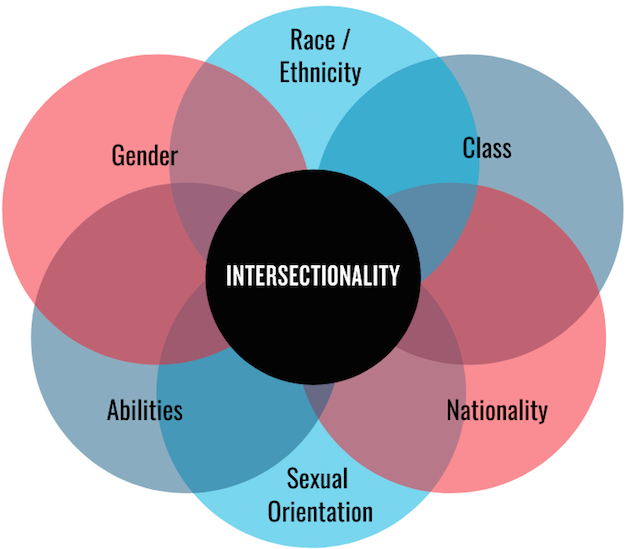
\includegraphics[width=2in]{fig/intersect.png}
% \caption{Some important intersectional
% categories.}\label{intersect} 
% \end{wrapfigure}  Another dimension of ``braodness'' is that this project must work with individuals across the spectrum of what
%  Crenshaw calls ``the interconnected nature of
%  social categorizations as they apply to a given individual or group, which overlap creating 
%  unique systems of disadvantage and discrimination.''~\cite{crenshaw2017race}.
%  No single project can address the vast
%  problems of discrimination addressing   society.
%  But given the importance of those problems, any projects (like this one) should
%  see themselves as  morally-required
%  to make a serious exploration of at least some
%  of those issues.
%    NCState has numerous faculty  from number intersectional grouping, all    actively exploring issues of social justice as well as extensive     out-reach programs to many   community groups. We look forward to a close association  such groups, including running case studies
%    with individuals from groups who,
%    traditionally who have been assigned seen much more (or much less) that their fair share of
%    social resources.  Note that for this category,   we   need to match
%    those individuals with models addressing social justice issues (e.g. see the social justice example,   offered above).
 

% \subsection{Engineering Questions}
% {\em Engineering questions}   speaks to the practicality of building a system like {\ITTT}.
%  \subsubsection{  RQ1:  How to collect the  extra advice in a cost-effective manner?}
 

 
%   The Achiles heel of any method that used background knowledge
%  is  how to acquire and apply that background knowledge. In this regard, in theory, our proposal is somewhat stronger than most:
%  \bi
%  \item It  is based on publicly available information about stakeholders
%  (see Table~\ref{info}). 
%  \item Further, we note
% that if we ever have problems using pre-existing data, it could
% also be possible to conduct specific data collection exercises,
% just for this project, 
% Given team members belonging to a
% team for more than a few days, it would be practical for each team member to spend an hour running {\ITTT} on some small canned examples
% that reveal that team member's attitudes
% and preferences to across different parts of
% the policy space within models like (e.g.)
% Figure~\ref{fig:scrumModel}.
% \ei
% As to the process of mapping
% that background knowledge to the terminology of our models,
% much of that technology is readily available~\cite{novielli2018benchmark,Burstein19}. Further, this research team
% has had much recent success with applying natural language processing techniques,
% even to large quantities of  SE data~\cite{Agrawal_2018,majumder2018,Agrawal19z,MenziesM08}\footnote{E.g.  \cite{MenziesM08} was honored as a distinguished ``test of time'' paper at ICSME'19. \cite{majumder2018} showed how to speed  up NLP on StackOverflow
% data by three orders of magnitude. \cite{Agrawal19z} discussed methods of how to very quickly tune and improve these NLP techniques.}.


% That said, it remains to be seen if this work will be as simple as suggested above. Hence we say:
% \begin{formal}
% {\bf Success Criteria \#1}: For
% this research to succeed, we will need to show that it is   fast and simple
% and scalable to   map user knowledge like Table~\ref{info}  into the terms used in 
% specific models. 
% \end{formal}
 

% \subsubsection{   RQ2:  
%   Does this extra advice change the
%   reasoning?} 
%    The   premise of this work is
%   that we can change what is discovered by PSO by flying the particles around a cloud of examples  
%   annotated with sentiments like "great place! come try over here!" or
%   "terrible place! please try to avoid!". 
%  This research question needs to check that premise using multiple models and multiple user sessions. 
%  \begin{formal}
% {\bf Success Criteria \#2}: 
% The results from PSO are statistically
% significantly different with and without using background 
% knowledge encoded as annotations over
% the decision space.
% \end{formal}
 
 
 
%    \subsection{Negotiation Questions}
% {\em Negotiation issues}    speak to the complexity   handling multiple trade-offs between multiple people.
    
% \subsubsection{ RQ3: Are ``acceptable'' solutions   ``better''?}
% If we listen less to AI and more to humans,
% does that mean we have to compromise
% our optimization goals in order to appease
% more people? To say that another way,
% given the above definitions, 
% are ``better'' and ``acceptable'' opposing goals?

% The evidence so far is ``no''. In the   experiments with iSBSE conducted by 
% Lustosa~\cite{lustosa21,lustosa22}, they compared
% their human-in-the-loops 
% results (with {\ITS{0}}) against state-of-the
% art iSBSE methods~\cite{lustosa21}
% and SBSE algorithms (that made no
% use of human advice at all~\cite{lustosa22}).
% In those experiments:
% \bi
% \item
% Humans only
% ever commented on a small fraction of the state space (e.g. in
% Figure~\ref{fig:scrumModel},
% less than 
% 20 binary questions within a space of
% 128 options; i.e. less than $2^{20}\;/\;2^{128}$ of the state space
% \item
% While 
% {\ITS{0}} looked over a broader range
% of options that other methods\footnote{ Evidence for that claim: as mentioned above,
% {\ITS{0}} found better solutions than
% the prior state-of-the-art algorithms
% such   as FLASH or HYPEROPT and OPTUNA~\cite{bergstra2015hyperopt,nair18,akiba2019optuna} and 
% an iSBSE tool from  Araujo et al.~\cite{araujo2017architecture}.}.
% \ei
% Hence, {\ITS{0}}'s solutions were 
%    {\em acceptable} to humans
% and also {\em better} (as judged by the $y$ objectives). That said, this question needs further work since the {\ITS{0}} results were based on just a few models.

%  \begin{formal}
% {\bf Success Criteria \#3}: 
% Models found by {\ITTT} are both objectively ``better'' as well as being subjectively ``acceptable'' to our human stakeholders.
% \end{formal}
%  \subsubsection{ RQ4: How much advice
%  is too much?}
%  We believe that there is some ``negotiation cliff''
% after which all the tools described here
% will fail to find any consensus. Such failure is readily detectable within our PSO framework:
% \bi
% \item If   particles can   find solutions acceptable to most parties, then  they will converge to a few small regions.
% \item
%  If    stakeholders are implacably opposed, then   particles from converge
%  to very different locals in $x$-space.
% \ei
% With this measure of the output space,
% we can use our sentiment analysis tools
% to measure the initial set of disagreement between stakeholders.  Our belief, to be confirmed  this experiment, is that a graph of initial {\em sentiment distance}\footnote{Take 100 terms are random from the domain. Submit as input to sentiment tools looking at the electronic footprint of different stakeholders. Count how often the same term gets the same sentiment from different stakeholders.}
% versus {\em final particle convergence}
% will reveal the location of the negotiation cliff. With this information, we can say:
% \begin{formal}
% {\bf Success Criteria \#4}: 
% We can recognize the point of negotiation
% failure .
% \end{formal}
% \noindent (e.g. via the negotiation cliff or some other measure we will develop as part of this work.)
% \begin{formal}
% {\bf Success Criteria \#5}: 
% Before the point of negotiation failure,
% we can still help stakeholders to find acceptable and better solutions over a wide range of model.
% \end{formal}

%  \subsection{Cognitive Questions}
% {\em Cognitive issues}    speak to the methods to managing systematic
% biases in human reasoning.

%  \subsubsection{ RQ6: Can we mitigate for bias?}
%   To err is human\footnote{
%  Alexander Pope, {\em  An Essay on Criticism}, 1711.}.
% Faulty conclusions  arise from algorithms (e.g. {\ITTT})  using  faulty human advice. How to mitigate for that faulty advice?

% This is an important problem.
% As mentioned above,   humans have fixed and limited attention spans 
%    which they  have learned to hoard and use sparingly~\cite{davenport2001attention}.
% Hence, humans  use heuristic ``short cuts'' that let 
% them satisfy the demands of their work, just enough, before rushing off to their next
% task~\cite{simon1956rational}.
% Such heuristics are essential if humans are to tackle their busy workloads but,
% as Green warned~\cite{green2022flaws},
% these can introduce systematic
% cognitive errors in their conclusions.
% The Wikipedia page lists hundreds of 
% ``systematic patterns of deviation from norm and/or rationality in judgment''\footnote{\url{https://en.wikipedia.org/wiki/List_of_cognitive_biases}.}
% including:
% \bi
% \item
% A tendency to be  over- optimistic
% (thus over-estimating greatly the probability of undesirable outcomes);
% \item
% A confirmation bias where we listen more   to information that confirms our existing beliefs;
% \item
% An anchoring bias  that   overly influences us with the first piece of information;
% etc.
% \ei
% In turns out that, as shown in Table~\ref{tbl:sigh}, computers
% can be   biased. For example,
% if some social group is under-represented in training data,
% then the conclusions reached by a machine learning from that data
% can make ill-informed decisions about that group (e.g.
% African-American men might end up with a higher false positive
% rate in software predicting the probability of become
% a  future criminals~\cite{Machine_Bias}).

 

%    \begin{quote} {\em 
%    ...people (including experts) are susceptible to ``automation bias'' (involving)  omission errors—failing to take action because the automated system did not provide an alert—and commission errors—following the advice of an automated system even though it is incorrect and there is contradicting evidence.~\cite{green2022flaws}.}
%    \end{quote}
   

%   Can we show   that   knowledge does not harm the results achieved from that search process?
%   Prior to the {\ITS{0}} experiments, one concern we had was that AIs might be able to understand
%   more options than people, in which case the  more an iSBSE algorithm tuned itself
%   to human opinion,   the worse the generated solutions. 
%   This turned out {\em not} to be true. 
%   As mentioned above in \S\ref{eg}, co-PI Menzies
%   and his graduate student Andre Lustos~\cite{lustosa21,lustosa22}
%   found that, at least in the models they explored,
%   it was possible to change solutions
%   (to better match human preferences) while at the same time optimizing the $y$ goals (and to do so better and with fewer evaluations than state-of-the-art tools
%   such as FLASH or HYPEROPT and OPTUNA~\cite{bergstra2015hyperopt,nair18,akiba2019optuna}). That said, in all our work with human-in-the-loop modeling, we will always double
%   up on algorithm execution: 
%   \be
%   \item
%   Once using humans-in-the-loop 
%   \item And once again when we   ignore people and just apply    the top ranked recommendation found by the algorithm.
%   \ee
%   Here, in this research question, we  would be monitoring for the case where the   performance deltas seen in these doublings grows unacceptably large.
%    \ei
%   One interesting result from our prior wotj
%   One unique feature of our rig is that we can measure the impact of human preferences 
%  All the solutions generated by {\ITTT} cab  be score: \bi
%   \item Proportionally by  their distance to positive sentiment examples;
%   \item Inversely proportional by the their distance to negative sentiment examples;
%   \item And proportionally according to the $y$=goals
%   (and if there are multiple $y$ objectives, then we can still sort them using the Zitzler predicate of
%    Table~\ref{active1})
%   \ei



%  {\ITS{0}}   adjusts its conclusions based on feedback from the people it talks to. 
% If, at some later time, some oversight group wants to
% know {\em why} some solution was reached, they may not
% have access to the humans who guided the original search (e.g. they may not recall why they made that decision and/or they have left the organization).
% So how can {\ITTT} give oversight bodies the information they need
% to audit past decisions? And how to do that in a cost-effective manner? 

% {\ITS{0}}  trusted the answers it collected from humans.
% But human advice can be faulty. How can {\ITTT} recognize
% faulty answers and how to mitigate the negative
% effect of those faults?

%  {\ITS{0}}  only takes advice from one person--
% which means its conclusions can be unduly biased by the views
% of one person.
% {\ITTT} should listen to teams of people working some problems.
% But humans can be argumentative.
% If we accept   advice from multiple humans, will
% all that advice help or hurt {\ITTT}'s processing?  
 
% Further, and perhaps most importantly, 
% recalling Table~\ref{tbl:sigh},
% software-based decision making can exhibit bias.
% Models may attributes describing ``projected
% groups'' with special privileges (or, sadly, lack of privilege). For such models,  bias manifest when 
% the performance of a model is significantly different for different groups.
%  {\ITTT} needs bias motoring and bias mitigation operators
% to   adjust conclusions in order to better  empower   the disempowered
% sections of society who (usually) are not included in software design discussion.  
 
%  Lastly,  {\ITS{0}} used a set of tactics to guide its question asking. There are   many such tactics and {\ITS{0}} just
% explored the tricks of Table~\ref{advice1}. 
% {\ITTT} needs to explore that larger space of (many)  different tactics for reducing human workload. 



% For 
% by   weight pushes the mutations along the curret direction which the cognitive and social 
% %XXX lit review. active elarning. SSL
% Experiments like the above serve to explain the problems
% raised by Green in \tion{why}. Recall that Green warned that when
% humans are tasked with oversight to software, that oversight is often incomplete (omission errors and commission errors where reported results missed important results or wrong results based on missed contradictory evidence).
% Tho source of these problems is seimple to explain--  and that explaination holds for both humanand automatic method for search complex models.  In




% Recall also that Recall also that, in the above
% results, all the {\ITS{0}} mades its conclusions after exploring
% only $10^2$ options.
% This is an interesting number since the models explored by {\ITS{0}} have a much large search space.  For example,
% the SCRUM mode show above has $2^{128}$ options,
% of which only 2\% is valid.  Hence, the total
% space of options is $2^{122}$. Yet {\ITS{0}} only explored   $2^{20}/2^{124}\approx$ a trillionth of that   decision space.  Now a case could be made that 
% {\ITS{0}} is explore the {\em important}  one-trillionth
% of the total space (since it performed so well)


% of that s{\ITS{0}} has been compared
% to numerous other optimization algorithms and found to generate comptitive solutions


% explain those problems, we note
% that   
% when working with humans  on {\ITS{0}}
% project, we found that they only ever wanted,
% or needed, to comment on a small part 
% of the total sate space of our SCRUM model.
%   After being asked 
%  20 detailed questions about ``do you prefer {\em this}
%  to {\em that}''    (each described in terms of 4 to 5 attributes),
%  they usually pleaded to stop being pestered.
%  That experience 
 
 
% Lane \& Valerdi~\cite{Lane05} found he needed 3*3 hour meetings of a delphi panel to get subject matter expert
% consensus on the values within 20 columns and 50 rows  within a spreadsheet (of software project cost drivers). 
% And while exploring an preference solicitation method
% called {\em repertory grids}, Whyte \& Bytheway~\cite{Whyte96}, and Curtis et al.~\cite{curtis08} found they needed an hour to for humans to offer
% considered opinions of a nine examples, each scored on nine scales. 

% The entire process of the RGT can be time consuming, with some researchers reporting that 90 minutes were required to create a 9 x 9-inch repgrid [Whyte and Bytheway 1996]. 


% For this proposal, the most important thing about {\ITS{0}} is that it lets us explain   the effects that concerned Ben
% green in \tion{why}.  Some simple mathematics explains why.

% This fraction  $2^{20}/2^{128}$   explains at lease some of the issues
% documented by Green. XXX. iSBSE should be seen as an essential part of human+AI decision making:
% \begin{itemize}
% \item
%  iSBSE is essential  since
% it stops human preferences from being ignored. 
% \item To see this, recall the fraction $2^{20}/2^{128}$  of important preferences
% within our SCRUM model.
% When important user preferences fall within one-trillionth of the total
% space then, without iSBSE, it is vanishingly unlikely that a fully automated algorithm will select those
% preferred options.
% \end{itemize}

 
  
% % \begin{figure*}
% % \begin{subfigure}{.2\textwidth}
% %   \centering
% %   % include first image
% %   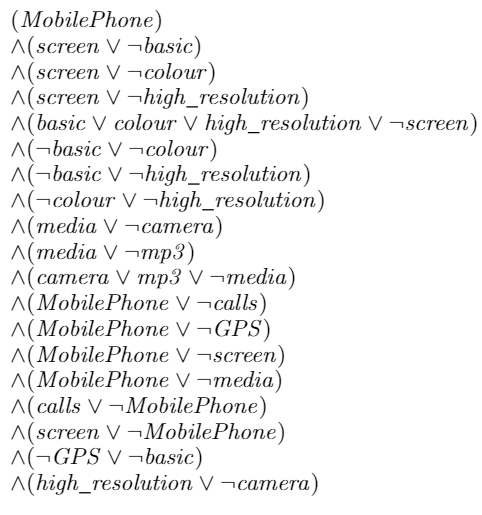
\includegraphics[width=.3\linewidth]{fig/CNF.png}  
% %   \vspace{1.06cm}
% %   \subcaption{CNF formula for  Figure~\ref{phone}. }
% %   \label{fig:PhoneCNF}
% % \end{subfigure} 
% % \begin{subfigure}{.2\textwidth}
% %   \centering
% %   % include second image
% %   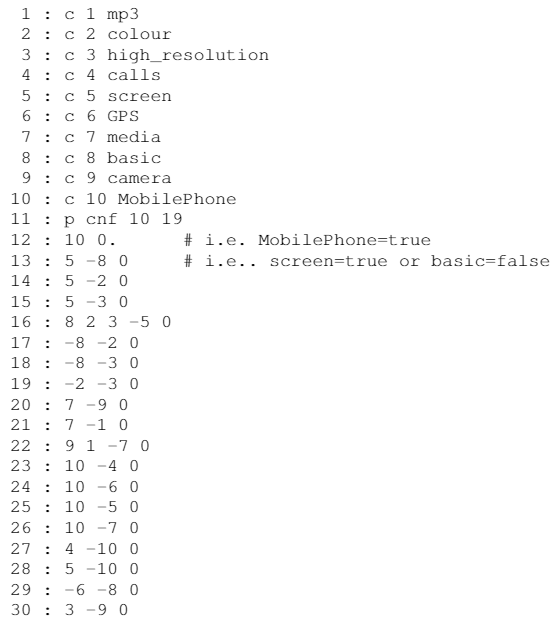
\includegraphics[width=.3\linewidth]{fig/dimacs.png}  
% %   \subcaption{The Dimacs representation\\ of Figure~\ref{fig:PhoneCNF}.}
% %   \label{fig:PhoneDimacs}
% % \end{subfigure} 
% % \begin{subfigure}{.2\textwidth}
% %   \centering
% %   % include second image
% %   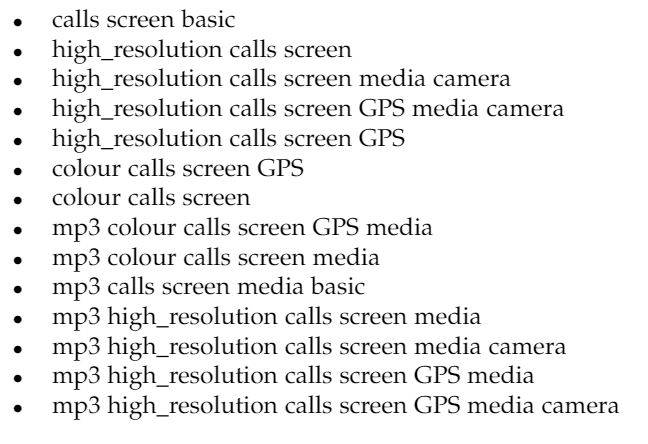
\includegraphics[width=.3\linewidth]{fig/Solutions.png}  
% %     \vspace{1.6cm}
% %   \subcaption{PicoSAT inputs Figure~\ref{fig:PhoneDimacs} to output
% %   multiple solutions. Each line shown here is one valid product extracted
% %   from the product line of Figure~\ref{phone}.}
% %   \label{fig:PhoneSolutions}
% % \end{subfigure}
% % \caption{In Figure\ref{fig:PhoneData}.b, line numbers added left-hand-side for ease
% % of reference). Lines 1 to 11 are comments, show variable names.
% % Line 11 reports that there are 19 clauses discussing 10 variables. After line 11, a ``0'' denotes the
% % end of a clause;
% % each clause is a disjunction, and all the clauses combine into one conjunction. 
% % Within each clause
% % negative numbers denote negation .}
% % \label{fig:PhoneData}
% % \end{figure*}





% In this proposal, we describe the limitations of  {\ITS{0}} 
% and argue that those limitations are common to a broad class
% of   iSBSE algorithms. 
% More specifically, current  work in interactive search-based SE,
% including {\ITS{0}}
% does not adequately
% address:
% \bi
% \item
% The  {\em social issue} of bias mitigation
% associated with advice-giving algorithms;
% \item
% The 
% {\em negotiation issue} of how to handle advice from multiple experts;
% \item
% The {\em cognitive issue} of how to recognize and repair faulty advice from a human;
% \item
% The
% {\em engineering issue} of how to find the advice 
%  (in a cost effective way) needed for this   reasoning; 
% \ei
% The goal of this research is to create {\ITTT}, a tool
% that resolves all those open issues.
% A key feature of {\ITTT} is that it is an open framework that can  accept advice  from multiple sources of knowledge in order to guide its thinking. This advice can be the usual knowledge sources (e.g. data miners running on SE project data) but, in the extension explored here, this advice can also include preference and goal information. For example, suppose we know:
% \bi
% \item
% The design documents;
% \item
% Which parts of those documents have been most edited by particular designers;
% \item
% The social media posts written by our designers;
% \item 
% The  prior decisions made by members of this design team engineering;
% \item
% The prior decisions made by teams of designers working on similar problems.
% \ei
% From that  record, we could use (e.g.) natural language processing techniques to find the ``hot button issues'' for those  designers. Examples of such hot button issues might be ``use open source licenses'' or ``minimize energy requirements'' or  ``avoid bias and discrimination''. 
% With  that knowledge of the beliefs and desires, {\ITTT} can change its conclusions to conform to the needs of different humans. 





% \section{Related Work black blah}
% This work draws on many sources.
% Semi-supervised learning methods try to label as few examples as possible in order to achieve some goal.

% Since 2012, active learning approaches have been received scarce attention in SE~\cite{kocaguneli2012active,tu2020better,yu2019improving,yu2020identifying}.
% Initially, it seems to be   a   promising method for addressing the cost of label checking and generating.
%  For self-admitted technical debt identification, only 24\% on the median of the  training corpus had to be labelled~\cite{yu2020identifying};
% Also,  using active learning,
% effort estimation for $N$ projects only needed labels on    11\% of those projects~\cite{kocaguneli2012active};
% Further, 
% while seeking 95\% of the vulnerabilities in 28,750  Mozilla Firefox C and C++ source code files,   humans only had to  inspect 30\% of the code~\cite{yu2019improving}.
% That said,  after much work, it must be reported that 
%  active learning still produces disappointing results.
%  It is still   daunting   to
% ``only''  label (say)  5\% to 2.5\% of the projects in the   1,857,423 projects in RepoReapers~\cite{curating} or
% the 
% 9.6 million links  explored by Hata et al.~\cite{Hideaki19}.


% From 
%  requirements engineering , this work addresses shortcomings with 
% Easterbrook, Nuseibeh and
% Finkelstein~\cite{easterbrook1994coordinating}
%  ``viewpoints engineering'' where   a large quantity of information collected from many different sources is
% partitioned into consistent sets, then  reasoned about separately. 
% Easterbrook   notes the complexity of that approach: making final decisions by merging viewpoints proved more complex than expected~\cite{easterbrook2005viewpoints}. Hence
% we prefer the PSO framework described above where
% merging ideas from different sources is done
% continually by each individual particle.

% A more fluid representation of domain models
% comes from the soft goal   framework of Chung, Yu,   and Mylipolous. et al.~\cite{chung2012non}.
% Unlike hard goals, which much be satisfied,
% sets of software goals need only be partially
% satisfied (and one solution is better than another if it satisfies the most parts of the most softgoals). But like viewpoints,
% soft goal researchers found it hard to negotiate a final solution. We have conducted studied with standard softgoal resolutions methods versus
% \ITS{0} (a prototype there was precursors to {\ITS{0}}).
% For example, Horkoff and Yu~\cite{Horkoff11}
% discuss local propagation methods for reasoning backwards from goals or forwards from assertions across softgoals (and sometimes, the Horkoff and Yu methods call SAT solvers as a sub-routine).
% We found that \ITS{0} (that stochastically grabbed some random examples as the seeds of a set of solution clusters, then growing beliefs from there), does much  better  and runs much faster than     softgoal methods. One reason to
% prefer  {\IT} over Horkoff and Yu's methods is that we can reach our conclusions with less questions to the user.


% % TABLE OF TECHNIQUES
% \begin{table}[t!]
% \caption{Note: Search Techniques Seen Used in iSBSE.}\label{tab:papersPerSearchTechnique}
% \small
% \centering
% \begin{tabular}{lllllll}
% \hline
%                                        ID & Single Objective & Multi-objective & Many-objective & Other & Example system\\ \hline
% 1 & \textbf{Exact}                         & 4.1\%            & 0\%             & 0\%            & 0\%    & \cite{palma2011using}\\
%  & \textbf{Metaheuristic}                 &                  &                 &                &       & \\
% 2 & \textit{~ ~ ~Single-solution based}   & 4.1\%            & 0\%           & 0\%            & 0\%    &\cite{lin2016interactive}\\
% 3 & \textit{~ ~ ~Evolutionary computation} & 61.5\%           & 20.5\%          & 4.1\%          & 4.1\%  &\cite{araujo2017architecture}\\
% 4 & \textit{~ ~ ~Swarm intelligence}       & 8.3\%            & 0\%             & 0\%            & 0\%    &\cite{do2016incorporating}\\ 
% \hline
% \end{tabular}


% \end{table}

% As to other interactive SBSE methods,
% Table~\ref{tab:papersPerSearchTechnique} shows a literature review on recent papers in that field~\cite{lutosa21}.
% That review found 40 most-cited
% iSBSE papers at senior SE venues (TSE, ASE, SSBSE, ACM, and others). The percentages in that table shows what percent of papers explored which approach.   One pattern we have seen in that literature is that many iSBSE
% papers seem weak on  scalability. For example, the biggest model
% processed by Palma et al.~\cite{palma2011using}  has 50 variables and not that many constraints. 
%  One reason to
% prefer  {\IT} over other iSBSE methods is that our data mining operators (from Table~\ref{advice1})   reach our conclusions with very few questions to the user. From the iSBSE literature, the closest we have
% seen to our work is:
% \bi
% \item
% The ``Swarm intellgience architecture'' from   Ferreira et al.~\cite{do2016incorporating}  that  changes its search approach on the feature space and provides the user with a candidate solution. On each interaction, the user can either accept the solution, terminating the algorithm or they can reset their preferences for each of the model's features to query for a different solution. We do not use the Ferreira et al. methods
% since they report some interesting challenges
% in their results. They report an average decrease of 13\% in their 50 feature model experiments' maximum performance score, whereas their technique was only able to reach 13\% of the best solutions generated by their methods.
% \item  Araújo et al.~\cite{araujo2017architecture} combination of  
% a genetic algorithm with a neural net,
% where the former does the  optimization and the the latter learns a classifier that guesses if its users will like or dislike the next example. Lustosa et al.~\cite{lustosa21} has compared {\ITS{0}} with the methods of Araújo et al
% and found that our data mining operators prune the search much faster, and produce better solutions.   We attribute the success of {\IT} in this context to the following. {\IT} maps out the shape of the data, then jumps to the regions of densest information. This is a more informed search than the arbitrary mutations used in 
%  Araújo et al. approach.
%  \ei


%  Finally  over-arching issue for all
%  the above iSBSE methods  is that they do not handle the concerns raised in
%  \S\ref{bad};  e.g  ``how to handle opinions from multiple people`` and 
%  ``what to do if the advice from people is faulty?''. Accordingly, we are motivated to look further afield at other technologies. Hence this proposal.
  

% \section{Research Questions}
% \begin{formal}\noindent
% {\bf RQ1:} Can we access sample models?
% \end{formal}

% asdads


% ADVICE-1 has been benchmarked against a state-of-the-art
%    iSBSE algorithm~\cite{araujo17} that uses genetic algorithms and neural networks (the former manages
%    the search, the latter builds a surrogate model that can answer  more questions,  faster, than people can). It has also been compared
%    to standard multi-objective-optimizers   Grid search~\cite{bergstra2011algorithms}, random search~\cite{bergstra2011algorithms}, differential evolution~\cite{storn1997differential}
%    FLASH~\cite{nair2018finding}, HYPEROPT~\cite{bergstra2015hyperopt}, and OPTUNA~\cite{akiba2019optuna} 
   
% ADVICE-1 addressed {\bf GOAL1} by first  recursively  clustering of all the

% things we could then, then asking about the issue that clarifies
% most issue More specifically, generate a binary tree whose
% nodes split the data into sibling sub-trees $t_1,t_2$ containing examples
% $n_1,n_2$. Examples have independent and dependent attributes
% and the find the largest sublings    goncaining 
% for the largest nodes with least variance\footnote{More precisely, variance for numeric attributes and entropy for symbolic attributes.} ask about issues
% that distinguish that node from its sibling in the tree).
% • ADVICE-2 mist not ask humans too many questions. To that emd, this research will empirically evaluate
% dozens of different tactics for find the fewest, most informative questions.

% DVICE-2 adjusts its conclusions to the needs of the people using it. To collect that information in a
% cost-effective manner (in a way that is verifiable and auditable), we will use natural language processing
% tools.

% • Human advice can be faulty. Using meta-patterns of faulty behavior, we will recognize when this advice
% is helping, not hurting, our ability satisfy more goals.
% • Humans can be argumentative. When we accept advice from multiple humans, we will clustering that
% advice to find maximal subset of ideas (within which the most users agree on the most things).
% • We will define monitoring tools to ensure they we are not excessively clustering models and data (which
% lets us mitigate for situations where conclusions compromise too much, thus satisfying no one).
% • ADVICE-2 uses bias motoring and bias mitigation operators to change conclusions in order to better em-
% power disempowered sections of society who (usually) are not included in software design discussion


% \subsection{Research Questions}
% The above line of reasoning, and our experience with {\ITS{0}}, leads to several research questions.

% RQ1: is  ADVICE useful? I.e if we accept human advice, does that lead to solutions that satisfy more goals?



 
% \subsection{Other Details}
% This NSF solicitation has certain required
% headings. Much of the information needed for those headings
% has already been presented. That said, we aggregate that information here.

% \subsubsection{Results from prior CSSI awards}

% This proposal is based on prior results generated from
% Elements: Can Empirical SE be Adapted to Computational Science? Award \#1931425
% (PI= Dr. Tim Menzies, NCState. 2019-2022).
% Problems with COVID   meant that we could
% not attend enough CSSI meetings to contact more groups.
% That said, using telecommunication tools,
% we spend much time interviewing CSS developers looking for their specific project needs.
% Samples of results from that CSSI were presented in 
% \fig{health} and 
% Table~\ref{casestudy}. 
 

% \subsubsection{Cyberinfrastructure Plans}

% As said in our introduction,  
% a unique feature of this proposal is its scope.
% All the tools generated by this  project  will  be  placed  on-line  in  a  free-to-access  Github  repository  and  made  available  to  the  CSS community via an open source license.
% The software produced here will be applicable to  {\em any} CSS project using an open source repository (and we know at least 700 such projects). In our concept of operation 
% for any project  registered  with {\IT},
% whenever developers commit code, they automatically receive an issue report commenting on the current and future health of their software, along with advice on how to improve that future state.  
 
%  \subsubsection{Measurable Outcomes}
% In terms of measuring the success of this work,
% those  
%  \textcolor{red}{{\bf measurable outcomes}} are listed in red (see above).
 
%  Also,  all the code developed as part of this work will be  released as open-source software in GitHub, under an MIT license.  Included in those
% packages will be the data used to certify the scripts as well as {\em RQn.sh} files containing executable scripts to reproduce (e.g.) RQ1.



%   \subsubsection{Management and Coordination Plan}
  
%   As said in our introduction, it is not enough to merely advertise some service and expect the community to use it. Much of the funds requested by this work is for  NC State researchers  to 
%   analyze as many CSS projects as possible. With these preliminary results in hand, they will approach CSS projects offering commentaries on their software (derived via our data miners)  and free consulting services on how to improve those projects. By  enticing CSS project members with results from their own projects, we anticipate growing a large user base amongst the CSS community.
  
 

 

%  \subsection{Related work in the Explanation Literature}
 

% When discussing this work with colleagues, they sometimes comment that
% xPLAIN is more a ``planner'' (on what to change) than an   ``explaination''
% device.
%  To those colleagues,
%   we  reply that there
%  is
% much precedent in the AI literature
% for connecting planning to explaination.
% In their systematic literature review on AI and explanation, 
%  Violane et al.~\cite{vilone2020explainable} use terminology that we find to be synonymous with our
%   plans that recommend what to change in order to most improve a system.  Violane et al. report is that
%   one of the 
%  most widespread use of explanations
%  in AI is to  find ways to change a
%  models behaviour; e.g. to debug a system in order
%  to stop some bug reoccurring).  
 
%  Other researchers make analogous conclusions.
% Adadi and  Berrada~\cite{Adadi18} list
% four main motivations for building
% explanation systems: 
% (a)~{\em explaining to justify} decisions made
% by some  model;
% (b)~{\em explaining to control} a system,
% allowing its debugging and the identification of potential flaws;
% (c)~{\em  explain to improve} 
% predictive performance and/or efficiency;
% and 
% (d)~{\em explaining to discover} novel  relationships and patterns in the data. As shown by the examples
% below, our ``planning as explanation'' methods  address motivation (b,c,d).

% Furthermore, the Violane et al. review
% lists no less than 37
% terms connected
% to current AI papers discussing  ``explaination''\footnote{
% Algorithmic transparency, 
% actionability, 
% causality, 
% completeness, 
% comprehensibility, 
% cognitive, 
% correctability, 
% effectiveness, 
% efficiency, 
% explicability, 
% explicitness, 
% faithfulness, 
% intelligibility, 
% interactivity, 
% interestingness, 
% interpretability, 
% informativeness, 
% justifiability, 
% mental fit, 
% monotonicity, 
% persuasiveness, 
% predictability, 
% reversibility, 
% robustness, 
% satisfaction, 
% scrutability / diagnosis, 
% security, 
% selection/simplicity, 
% sensitivity, 
% simplification, 
% soundness, 
% stability, 
% transparency, 
% transferability and, 
% understandability}.
% Semi-supervised planning relates to at 
% least two of the terms in the  
% Violane et al. survey: actionability and  effectiveness (since both these terms comment on if a plan can be deployed and (after that) how well the plan actually works.

  
 
 
 
 

\subsection{BPC Work: Broader Participation in Computer Science} \label{bpc}
\noindent
(For all our BPC details, see {\em Supplemental Documents ``Broadening Participation in Computing (BPC) Plans''}.)

NC State’s Computer Science department has a distinguished history of overcoming barriers faced by women, and advancing methods to broaden participation in software engineering. This commitment is not merely historical; it is the driving force behind ongoing initiatives. In particular, 

\bi
\item
The curriculum and lecture notes of graduate SE and HCI classes, led by PI Menzies and co-PI Sandeep Kuttal,  will be meticulously revised to embed content for {\IT} and addressing gender bias and promoting inclusivity with it's design. 

\item Funding from this effort is earmarked to support students attending prominent diversity conferences such as the Grace Hopper conference and the Richard Tapia Celebration of Diversity in Computing.
\ei

Significantly, some of this grant will be allocated to bolster the department’s Broadening Participation Committee (BPC), where both PI Menzies and co-PI Kuttal actively contribute. This BPC team explores  factors influencing the attractiveness of computer science to underrepresented groups. Dr. Kuttal, specializing in gender and race research, has an impressive track record, advising 35 undergraduates (including 12 women) and 4 MS students in her prior role at her prior institute. At NCSU, she currently advises 2 PhD students, including 1 Black woman, and 14 undergraduates, of whom 7 are women. Her mentoring extends beyond the classroom, holding leadership roles in organizations like the Society of Women Engineers (SWE) and the National Center for Women in Information \& Technology (NCWIT).

Metrics for the BPC plan include   number of students supported to travel to conferences;  and an evaluation of the ADVICE project for inclusivity using   GenderMag   (gendermag.org). Dr. Kuttal’s involvement in Gender research is notable, contributing to reducing bias in software engineering (e.g.~\cite{Kuttal2021g, Kuttal2019, Alexposter2022, KuttalKMB21,Robe2020}). PI Menzies, a member of the BPC, is committed to understanding factors affecting diversity and continuing his tradition of graduating research students from historically underrepresented groups.

Specific BPC activities supported by this work include the creation and extension of BPC-oriented lecture notes for various NSF-funded REUs (research experience for undergraduates) and graduate SE classes. Additionally, funds will be directed to support students attending key diversity conferences. This comprehensive plan underscores flexibility for adjustments based on ongoing feedback and evolving needs, maintaining transparency in communication to the academic community.


%The BPC plan for NC State’s Computer Science department aims to promote inclusivity and diversity in software engineering, building on the department's longstanding commitment to studying gender bias, barriers faced by women, and methods for broadening participation. The plan encompasses a multi-faceted strategy, including the revision of graduate SE classes' curriculum to incorporate content addressing gender bias and inclusivity, financial support for students attending key diversity conferences (attending the Grace Hopper conference, and the Richard Tapia Celebration  of Diversity in Computing) , and allocation of funds for BPC Committee initiatives focused on attracting underrepresented groups to computer science. Dr. Sandeep Kuttal, co-PI, plays a pivotal role in mentoring and outreach activities, extending beyond the classroom to advise underrepresented students. The success of the BPC efforts will be measured through quantifiable metrics, such as the number of students supported to attend conferences and the evaluation of inclusivity in the ADVICE project using the GenderMag method. Both PI Menzies and co-PI Kuttal have distinct roles, ensuring active engagement and oversight. The plan emphasizes flexibility for adjustments based on ongoing feedback and evolving needs while prioritizing transparent communication of progress to the academic community.

 %NC  State’s  Computer  Science  department  has  a  long  tradition  of  studying research issues related to gender bias,  barriers faced by women, and methods for broadening participation    in  the  context  of  software  engineering. This work will continue that tradition.
%Curriculum  and lecture notes of the graduate SE classes (taught by PI Menzies and  co-PI Sandeep Kuttal ) will be revised from this work. Funds from this work will be used to support students attending the Grace Hopper conference, and the Richard Tapia Celebration  of Diversity in Computing. Furthermore,  a (small) portion of this grant would be allocated to support Broadening Participation in Computing (BPC) work.   PI  Menzies and  co-PI Kuttal are  members  of  their  department’s Broadening Participation Committee (BPC) which actively seeks to:  (a)~Understand what factors make computer science more (or less) attractive to underrepresented groups; (b)~Educate faculty, staff, and students on how different behaviors affect diversity, quality, and inclusiveness; (c)~Increase the percent of students who identify as women, and (d)~Evaluate the success of this BPC team in broadening participation. 


% BPCwork is strongly supported by PI's department
% (NC State's Computer Science).
% Our department
% has a strong record of studying research issues related to gender bias~\cite{pullreq_17}, barriers faced by women ~\cite{ford2016paradise}, and methods for broadening participation~\cite{selfies} in the context of software engineering. 

%Co-PI Kuttalis very active in the GenderMag research, working towards reducing bias against women and other social groups in SE~\cite{Kuttal2021g, Kuttal2019, Alexposter2022, KuttalKMB21,Robe2020}) as well as involved in leading Society of Women Engineers (SWE), and NCWIT at the university and community level.   PI Menzies is a member of his department's Broadening Participation Committee (BPC) that actively seeks to understand  factors that make computer science less attractive to underrepresented groups, then educate faculty, staff, and students on how different behaviors   affect diversity, quality, and inclusiveness. Also, PI Menzies will continue his established tradition of graduating research students for historically under-represented groups.
  


%BPC activities supported by this work will be:
%\bi
%\item The creation and extension of BPC-oriented   lecture notes of the various NC State NSF-funded REUs (research experience for undergraduates) as well as graduate
%SE classes (taught by PI Menzies and co-PI Kuttal).  
%\item
%Funds from this work will be used to support students attending the Grace Hopper conference, and the Richard Tapia Celebration  of Diversity in Computing.
%\ei
 

 
\subsection{Dissemination of Knowledge}

All the code developed as part of this work will be  released as open-source software on GitHub, under an MIT license.  Included in those
packages will be the data used to certify the scripts as well as {\em RQn.sh} files containing executable scripts to reproduce (e.g.) RQ1. If this research proves successful, the NAS team would be using these tools as part of their SMART-STEReO work.

  As to papers, the PIs of this grant
  frequently published in top-ranked international scientific venues.
Using those forums, the PIs will evangelize {\IT} in the software industry.  The results of the research and educational activities will be disseminated widely via publications and conference presentations, as well as software that will be used by researchers and educators.
    

Also, this work will generate much  material (tools, scripts, data sets) that can be utilized by other research teams. 
For  a decade, PI Menzies has  lead-by-example in the open science community (the PROMISE project and the ROSE initiative) which takes care
not only to package and distribute research code but also to publish papers and tutorials on that material.  
 


 
 \section{Prior Results}\label{sec:PriorResults}
 

 
PI Menzies is an IEEE Fellow and has earned over \$13 million dollars in peer-reviewed competitive grants (\$6.4M from NSF, and  the rest from a variety of other government and industrial sources).
Google Scholar lists him as a top-ten researcher in many research areas including knowledge acquisition and analytics. Serving as committee chair, he has graduated 18 Ph.D. and 32 master students (by research). He currently supervises 10 Ph.D. students at NC State. He has served as an associated editor on all the major SE journals and from 2021 will be EIC of the Automated Software Engineering journal. 


Co-PI Kuttal has a long  track record of creating tools   supporting programmer creativity \cite{Kuttal2020}, exploratory programming behavior \cite{Jernigan2017, Jernigan2015}, debugging web-based distributed programming \cite{KuttalSR13-chi, KuttalSBRKS19}, % REMOVED: KuttalSR13
problem-solving techniques \cite{Jernigan2017, Jernigan2015}, gender-specific behavior \cite{Kuttal2021g, Kuttal2019, Alexposter2022}, socio-technical skills \cite{Abimposter2022,Abimgitposter2022,Diwanjiposter2022,Zhou2018, sarma2016hiring, KuttalCWBS21, KuttalSRW18, abs-1810-13062} and communication styles \cite{Kuttal2020}.  She is currently developing conversational agent for programmers \cite{Kuttal2020, Kuttal2021,tochipaper, RobeFSE2022, Robe2020, Hartposter2022, Alexposter2022}, supporting information foraging~\cite{Abimposter2022,Abimgitposter2022,Diwanjiposter2022}, and  studying developer's   interactions when problem-solving in same- and mixed- gender pairs.


 We include below notes on some of the most recent NSF grants.

% PI Menzies is a co-PI with    Dr. Laurie Williams  working  on \underline{(a)}~CCF-1909516, 2019-2022, \$499,998; \underline{(b)}~``SHF: Small: Detecting the 1\%: Growing the Science of Vulnerability Detection''; \underline{(c)}~The {\bf intellectual merit} of that work was to explore characteristics of vulnerabilities with a focus on those that pose the highest security risk. The {\bf broader impact} of that work was to improve the ability of practitioners to produce secure software products so that people can rely upon computer systems to perform critical functions and to process, store, and communicate sensitive information securely. \underline{(d)}~That work has generated   journal articles (one at TSE), ICSE publications and one paper under review (at EMSE) \cite{yu2019improving,shu2019improved,elder2021structuring,shu2020omni}. \underline{(e)}~Data from that work is housed at the SEACRAFT publicly accessible repository~\cite{seacraft}. That work funded two Ph.D.s at NCSU. \underline{(f)} N/A.

PI Menzies worked on \underline{(a)}~CCF-1302216, 2013-2017, \$271,553; \underline{(b)}~``SHF: Medium: Collaborative: Transfer Learning in SE''; \underline{(c)}~{\bf Intellectual merit: }  
define novel methods for sharing data.  That work generated the publications  \underline{(d)}~\cite{peters2015lace2,he13,Me17,fu2016tuning,krishna2017learning,krishna2020whence} concerning prediction and planning methods \cite{krishnaTSE18}. % REMOVED: krishna2018bellwethers
 {\bf Broader impact}:
enable a new kind of open science-- one where all data is routinely shared and is capable of building effective models no matter if it is obfuscated for security purposes.
The methods of this project, while targeted at SE, could also be applied to any other data-intensive field. \underline{(e)}~Data from that work is   housed in   two
publicly   repositories\footnote{
{\bf github.com/rshu/Adversarial-Evasion-Defense}}. That work  funded two Ph.D.s. \underline{(f)}
N/A. 


% One related data mining grant is \underline{(a)}~OAC-1931425, 2019-2022, \$592,129; \underline{(b)}~``Elements: Can Empirical SE be Adapted to Computational Science?''; \underline{(c)}~The {\bf intellectual merit} of that work was to create a workbench containing methods adapted from empirical software engineering, that would help bridge the skill gap via automatic agents by suggesting to developers when they should investigate or redo part of their code. The {\bf broader impact} is to reduce the associated cost (time, money, etc.) required to handle many of the large and more tedious aspects of software development. \underline{(d)}~That work generated one journal paper (at TSE), an MSR conference
% paper and two other papers under conference review~\cite{agrawal2018better,tu2021mining,tu2020changing}. \underline{(e)}~Data from that work is housed at the SEACRAFT publicly accessible repository~\cite{menzies2017seacraft}. That work funded one Ph.D. at NCSU. \underline{(f)} N/A.

Another relevant research grant is 
\underline{(a)}~OAC-1826574, 2018-2018, 
\$124,628;
\underline{(b)}~
``EAGER: Empirical Software Engineering for Computational Science'';
\underline{(c)}~ 
The {\bf intellectual merit} of that work was to
conduct initial explorations into novel methods for adapting SE methods to computational science.
That work lead to the curious
results that, in many ways,
the computational scientists are better
at managing their development cycle
than many SE projects~\cite{tu2020changing}. Whenever
we found good enough data to compare the results
seen in open source and computational
science projects, we often find higher productivity
values (and faster debugging) in computational science
than in software engineering. 
\underline{(d)}~That work generated 
one journal paper (at TSE'21),
one conference paper (at MSR'21) and another journal publication under review~\cite{Ling21}.
 \underline{(e)}~Data from that work is now housed at the SEACRAFT publicly accessible repository~\cite{menzies2017seacraft}. That work  funded one Ph.D. at NCSU. 
 \underline{(f)} N/A.  
 
 
 Co-PI Kuttal has received NSF CAREER and AFSoR YIP awards. Both projects are relevant to this project. Co-PI Kuttal is working on 
\underline{(a)}~ IIS - 204620, 2021-2026, \$ 520,522;
 \underline{(b)}~`` HCC: CAREER: Designing an Interactive Partner to Support Pair Programming''; 
\underline{(c)}~The {\bf intellectual merit} of that work was to create design guidelines for an anthropomorphic pair programming conversational agent \cite{Kuttal2020, Kuttal2021,tochipaper}, create initial set of 26 labels for programmer-agent conversations \cite{RobeFSE2022}, establish feasibility of using machine learning models\cite{Robe2020} and transformer-based language models for detecting programmer-agent conversations \cite{RobeFSE2022}, and establish feasibility of using online videos of pair programming sessions for training a pair programming conversational agent \cite{Hartposter2022, Alexposter2022}. 
The {\bf broader impact} of that work was to
enable a new kind of open science-- create an initial set of programmer-programmer and programmer-agent conversations.
\underline{(e)}~Data from that work is publicly available. That work funded one M.S. and one Ph.D., and two REUs at the University of Tulsa. Four other undergraduate students (2 women of color) worked on the research project. All students gained experience that crosses traditional boundaries of HCI, SE, and AI.
\underline{(f)}
N/A.

%That work generated the publications  \underline{(d)}~ \cite{ Kuttal2020, Kuttal2021,tochipaper, RobeFSE2022, Hartposter2022, Alexposter2022}.

Another relevant grant co-PI Kuttal is working on is \underline{(a)}~ FA9550-21-1-0108, 2021-2024, \$ 448,754\$;
 \underline{(b)}~`` Supporting Information Foraging by Utilizing Agents’ Collective Foraging Behavior ''; 
\underline{(c)}~ {\bf Intellectual merit:}  developed generic model for Question \& Answer website – Stack Overflow, foraging behavior of individual developers on GitHub and Stack Overflow\cite{Abimposter2022}.  It compared foraging patterns based on gender, specifically men and women.  We are currently developing models for GitHub \cite{Abimgitposter2022}, Stack Overflow, and web to help foraging for these heterogeneous sources to facilitate the foraging of newcomers \cite{Diwanjiposter2022}.
{\bf Broader impact:} allowed students to gain experience that crosses traditional boundaries of HCI, SE, and AI. The project funded one Ph.D. student at the University of Tulsa. Eight other undergraduate students (2 women of color and 1 man of color) also worked on this research project.
\underline{(f)}
N/A.

 
% HCC: CAREER: Designing an Interactive Partner to Support Pair Programming (IIS - 204620, for which Kuttal is the lead PI; 6/1/2021-5/31/2026, \$520,522), explores a variety of techniques to develop inclusive conversational agent for pair programming with Anthropomorphic properties by integrating diverse interaction mechanisms (visualizations, dialogue styles and agent actions), state-of-the-art machine learning algorithms, and creativity and problem-solving strategies. \textbf{Intellectual Merit:} The research has created design guidelines for an anthropomorphic pair programming conversational agent \cite{Kuttal2020, Kuttal2021,tochipaper}, created initial set of 26 labels for programmer-agent conversations \cite{RobeFSE2022}, established feasibility of using machine learning models\cite{Robe2020} and transformer-based language models for detecting programmer-agent conversations \cite{RobeFSE2022}, and established feasibility of using online videos of pair programming sessions for training a pair programming conversational agent \cite{Hartposter2022, Alexposter2022}.  \textbf{Broader impacts:} The work also provided gender-balanced labeled conversational data between human-human and human-agent for research community. The work supported one student who completed MS thesis and another student currently working on MS thesis.  It also supported 2 REU. Other four undergraduate students (2 women of color) worked on the research. All students gained experience that crosses traditional boundaries of HCI, SE, and AI.


%Other relevant grants is FA9550-21-1-0108, Supporting Information Foraging by Utilizing Agents’ Collective Foraging Behavior, 2/15/2021-2/14/2024). The project investigate the use of the past collective information seeking behaviors of individuals, specifically software developers, to tactically reduce the overhead of finding relevant information for newcomers working on similar tasks. \textbf{Intellectual Merit:} They developed generic model for Question & Answer website – Stack Overflow, foraging behavior of individual developers on software development hosting site GitHub that allies distributed version control or source code management using Git. Also compare foraging patterns based on gender, specifically men and women. Foraging behavior of individual developers on Question & Answer website — Stack Overflow\cite{Abimposter2022}. Also compare foraging patterns based on gender, specifically men and women. We are currently developing models for GitHub \cite{Abimgitposter2022}, Stack Overflow and web to help foraging for these heterogeneous sources to facilitate the foraging of newcomer developers \cite{Diwanjiposter2022}.\textbf{Broader impacts:} One graduate student and 8 undergraduate students (1 man of color and 2 women of color) were supported by the project.




 \newpage

% See also 
% \underline{(a)}~CCF-1703487; 2017-2021,  \$898,349.00; 
% \underline{(b)}~SHF: Medium: Scalable Holistic Autotuning for Software Analytics; 
% \underline{(c)} The {\bf intellectual merit}
% of that work  was that there exist previously unexplored ``short-cuts'' in the search space of control parameters of data miners. The {\bf broader impact}
% was that better learners could be created
% automatically via ``hyperparameter optimizers''
% that exploited those short-cuts. This in term meant
% that anywhere these learners were deployed, they could
% be deployed again with {\em greater} effect. 
% \underline{(d)}~This work generated five journal
% articles at TSE, EMSE, IEEE Software,  
% and one other article currently under review at EMSE~\cite{yedida2021simple,agrawal2020simpler,Yedida21,DBLP:journals/ese/YangCYYM21,menzies2021shockingly,xia2019sequential};  \underline{(e)}~Data from that work is now housed at the SEACRAFT publicly accessible repository~\cite{menzies2017seacraft}. That work  funded two Ph.D. at NCSU.  \underline{(f)}~N/A.
 


  

\end{nsfdescription}

\begin{nsfreferences}
 \pagestyle{empty}
\section*{References}
      \bibliography{kenrefs,proposal,ssl,suvodeep,old}
\end{nsfreferences} 

\begin{nsffacilities}
  

% \section*{Facilities From other Institutions}
% As stated in our {\em Collaboration Plan},
% we have unpaid collaborators from Facebook,  Microsoft,
% and IBM. Once this research develops viable
% unfairness measurement and mitigation methods
% for semi-supervised algorithms, these collaborators
% will grant us access to materials, to be negotiated, at their
% site. Apart from (potentially) being able to access
% models  behind the firewalls of model stores, an important
% facility these collaborators could offer is access to the subject matter
% experts that can test if the veracity of our
% artificially generated models.


% \section*{Facilities at North Carolina State University}
 
     
\subsection*{Offices:}
The project PIs  and Co-PIs 
have  
and offices in their   CS Department. This department
has adequate space to house all research assistants
working on this project. All offices are wired for high-speed network access.

The PIs' departments at  NC State provide the space and basic networking services to
carry out the experiments, secretarial and administrative support as well as general-purpose office equipment ({\em e.g.}, fax, photocopiers, etc.).

\subsection*{Lab Space}
The PIs have their own lab space at NC State.
e.g. PI  Menzies' RAISE lab (Real-World 
AI and SE) is a newly renovated space containing over 1,500 ft\textsuperscript{2} of research space and 
15 cubicles, a meeting space, printer, and wide screen projector. 

\subsection*{Compute Facilities}
Part of {\IT} will involve comparatively assessing different technologies. For that process, it will be useful to have some large-scale compute facility for \textit{CPU-intensive studies}.
 
At NCSU, students working on this grant will have access to a 108-node compute cluster named ARC with 2,000 cores (AMD Mangy-Cours), Infiniband QDR interconnect, per node power monitoring, GPUs and SSDs and parallel file system support,
which was funded by an NSF CRI that he is the main PI of together with 5 co-PIs.  
The ARC facility is providing local and remote researchers with administrator/root privileges for Computer Science experiments at a
medium scale. This allows any of the software layers, including the operating system and Infiniband switch network routing tables, to be
modified for experimental purposes, e.g., to experiment with different
network topologies.  For large-scale demonstrations, other 
facilities will be utilized (the HPC discussed below.


Additionally, NC State University provides a High-Performance Computing (HPC) facility as a part of the initiative to provide state-of-the-art support for research and academic computing. HPC system (called henry2) provides NC State students and faculty with entry and medium-level high-performance research and education computing facilities, consulting support and scientific workflow support. The HPC ecosystem consists of 1233 dual Xeon compute nodes in the henry2 cluster. Each node has two Xeon processors (mix of dual-, quad-, six-, eight-, ten-core, twelve-core) and 2 to 6 GigaBytes of memory per core. The total number of cores increases as more cores are purchased and now exceeds 10000. The nodes all have 64-bit processors. All HPC projects have the capability to run jobs using up to 128 processor cores for up to 48 hours and smaller jobs up to a week.

 \subsection*{Access to Models}

As described in section 3 of this research proposal,
this work will required extensive access to models
from the   SMART-STEReO group, lead by
Dr. Misty Davies
(NASA, Ames).

The   SMART-STEReO group has an established procedure for
sharing such models. In the COVID era, to enable remote work on that project, this group created policies
by which they can build laptop software with all the licenses and permissions needed to work securely
on these materials. Now it is routine for that group to have researchers working on those models, from
around the country, logging-in via those secure laptops.


%  \section*{Unpaid Collaborators}
 
%  This document contains letter s of 
%  collaboration from:
  
% \be
% \item Tim Menzies,
% North Carolina State University; PI
% \item
%   Anirban Mandal, RENCI, UNC-Chapel Hill; unpaid collaborator (see attached letter).
  
%   \item
%   Wolfgang  Bangerth, Colorado State University, unpaid collaborator (see attached letter).
% \ee
% These researchers were active in our prior CSSI work and offered much useful feedback on our direction
% (as well as case study material).
% We full anticipate that these collaborations will continue.

\end{nsffacilities}

  \pagestyle{empty}
\DataManagementPlan{data}
%XXX human data
\newpage

 \pagestyle{empty}
\section*{Project Personnel}
 
\be
\item Tim Menzies,
North Carolina State University; PI 
\item Sandeep Kuttal,  
North Carolina State University; co-PI 
\item 
Misty Davis; NASA Ames; unpaid collaborator
\ee

\newpage
%\pagestyle{empty}
 
\section*
{Collaboration Plan}

This proposal is a collaboration between:

\bi
\item The PI and Co-PI at North Carolina (Menzies and Kuttal);
\item A team of subject matter experts at NASA Ames, Mountain View, California (led by Dr. Misty Davies).
\ei

At NC State, Menzies and Kuttal work down the corridor from each other in the Computer Science Department.

\bi
\item Their work is divided into (a) building the AI optimizers and (b) studying the humans exploring those algorithms.
\item This division aligns naturally with the skill sets of Dr. Menzies and Kuttal, respectively.
\ei



At NASA Ames, this work will be based on the fmtool models already being built as part of the ongoing SMART-STEReO project, funded by another agency.


\subsection*{History of Joint Authorship on Research Papers}
 PI Menzies from NC State and Dr. Davies
from NASA Ames have a 13 year history of collaboration and 
publication. For three years in a row, Dr. Davies  took on Dr. Menzies' students at summer interns at Ames, and this lead to numerous publications \cite{gay2010automatically,krall2014learning, ttKrallMD15}. % REMOVED: krall2015gale

 
\subsection*{Site Visits}
Each year 
 the PI and Co-PI and their graduate students will   visit Nasa Ames
for two-day trips. During these visits, the team aims to immerse themselves in the NASA culture, engage with subject matter experts, and initiate discussions to discern pertinent and meaningful studies within the scope of this research.
%to sample the culture there, meet the subject matter experts, and discuss what kinds of case studies might be useful and meaningful within the context of this work.

\subsection*{Access to Software}

\underline{\bf Ames accessing NC State Software:}
In this project,  teams will be asked to
play a simulation game  (described in \S\ref{interfaces} where they must 
monitor a large number of drones. 
To simplify collaboration, this game will be run on-line and accessible via a web browser. 
For that game:  
\bi 
\item Its details and case studies will be evolved using input from the NASA Ames team.
\item At NC State, Drs Menzies and Kuttal will co-supervise the graduate student building that tool 
\bi 
\item with interface guidance from Dr. Kuttal;
\item and algorithm interface guidance from Dr. Menzies.
\ei
\ei
\underline{\bf NC State accessing Ames Software}
The Ames SMART-STEReO group has an established procedure for sharing models.   In the COVID era, to enable remote work on that project,
this group created policies by which they can build laptop software with all the licenses and permissions needed to work securely on these materials. Now it is routine for that group
 to have researchers  working on those models, from around the country, logging-in via those secure laptops.

\subsection*{Year-by-Year Plan}


As to collaboration with NASA Ames, the nature of that work will change over the course of   this project. 
\bi 
\item In the first year:
\bi 
\item 
Most of the work will done at   NC State.  Drs Menzies and Kuttal run small lab studies on simple problems with NC State student participants. In this stage,
the aim will be to debug the gaming interface and ensure it has the necessary connectivity to the optimizers.
\ei
\item In year2:
\bi 
\item NC State will extend its game simulator such that it can interface to the fmdtools models used at NASA Ames. We anticipate this to be a systems task comprising mostly programming at NC State.
\ei

\item 
Year3 will require the closest collaboration. Here,
NASA Ames subject matter experts will be running gaming
simulations, using the NC State tools.  To simplify
that process, all the NC State simulations will be web-based
(see above).
\ei

Table \ref{DGcreativity} outlines the comprehensive 3-Year Plan for three graduate students.

While both PIs will oversee the project's success throughout the three years, in Year 2 and 3, they will integrate lessons learned into their respective course curricula. Tim's course on AI for SE can incorporate tasks and evaluations as assignments, with usability considerations and elements of UI design included in SKK's HCI.

Over the course of three years, Misty will play a vital role by sharing fmdtool models of drone and SMART-STEReO project artifacts, providing valuable feedback on the models, and contributing to study tasks. Additionally, she will conduct studies with experts to evaluate the effectiveness of \IT.

\subsubsection*{Summer Internships at NASA Ames}
 NC State grad students funded from this grant will spend at least nine months at NC State. As for the other three months, they will  apply to the NASA
Ames summer internship program. If accepted there, those
students will be supervised at Ames by Dr. Davies
to create the fmdtools interface, all the while using input
from the local models.


\subsection*{Budget Considerations}

All of the above can be accomplished with the project budget. As mentioned above:

\bi 
\item All the work generating fmdtool models of drone   is  on-going work, funded by another agency as part of the SMART-STEReO project.
\item 
The NASA summer intern placements will occur only if our students get accepted into that program-- in which case they will receive salary from the NASA end (for 3 months). 

\item As to the other travel described above, our budget has sufficient funds to cover that.
\ei


\begin{table*}[!t] 
\caption{Overall 3-Year Plan.}
{\small
\begin{center} 
  \begin{tabular}{|p{1.9cm}|p{4.2cm}|p{4.2cm}|p{4.2cm}|}\hline  
        \textbf{}&\textbf{Year 1}&\textbf{Year 2}&\textbf{Year 3}\\
\rowcolor{blue!10}
Student 1 (Tim)&
Create game that include the safety reports, rules and regulations, conops to  extract rules and constraints for flying drones
&
Create \IT~models and CPU-Intensive evaluations
Create better \IT~model based on evaluation and CPU-Intensive evaluations&
Dissemination of the model on Git for researchers and practitioners.\\
 

Student 2
(Tim/SKK)&
Investigate prompt engineering and terms
CPU-Intensive and Human-intensive evaluations 
&
Improved  \IT~ tool and 
Human-intensive evaluations 
&
Dissemination of the Tool on Git for researchers and practitioners.\\
 

\rowcolor{blue!10}
Student 3(SKK)&
Create the \IT~interface prototype and conduct Human-intensive studies with students &
Create \IT~ tool by integrating the model and conduct Human-intensive studies with students 
 &
Improved  \IT~ tool and conduct Human-intensive studies with experts\\
\hline

         \end{tabular}
  \label{DGcreativity}
  \vspace*{-18pt}
\end{center}}
\end{table*}







% \newpage

% \rhead{~}
%   \cfoot{~}
%   \lhead{~}
   
%   \pagestyle{empty}
% \section*{Delivery Mechanism and Community Usage Metrics}
% \pagestyle{empty}
% Note that, in the following, {\bf Goal4} will hold our community usage metrics.
% Also, all this information appears in the body of our project description (and we repeat that information here, just for completeness).


% \subsection*{Deliverables} All our scripts, all our data, source code
% for all our publications, anything we use in this project will be freely available on-line
% (in Github).

 
 
%  {\IT} will be an open source tool with ``hooks'' into source code repository system such as Github.    All the tools generated by this project will be placed on-line in a free-to-access Github repository and made available to the CSS community via an open source license.

% A unique feature of this proposal is its scope. The software produced here will be applicable to  {\em any} CSS project using an open source repository (and we know at least 700 such projects). In our concept of operation, 
% for any project  registered  with {\IT},
% whenever developers commit code, they automatically receive an issue report commenting on the current and future health of their software, along with advice on how to improve that future state.  

% NC State researchers will apply {\IT}   to as many CSS projects as possible. With  preliminary results in hand, they will approach CSS projects offering commentaries on their software (derived via our data miners)  and free consulting   on how to improve   projects. By  enticing CSS project members with results from their own projects, we anticipate growing a large user base amongst the CSS community.

% \subsection*{Metrics}
% {\em {\bf Goal1}: predict project health for some CSS projects}:
% We would generate the \tbl{med_mre}
% error measurements,  but for CSS
% projects.  Saro et al.~\cite{sarro2016multi} comments that for software project management, these errors should be less than 25 to 50\%. Hence we would say {\bf Goal1}
% is achieved if we can make low predictions with that kind of error.


 
% {\em {\bf Goals 2}: plan effective improvements for some CSS projects}:
% Given the tactics of Page~\pageref{tactics2},
% we would have different outcomes for different tactics.
% For   tactics 1,2,3  we can assess the results of our interventions using the  
%     {\bf a,b,c what-if procedure} defined   at the end
% of \S\ref{mm}
% (on page \pageref{abc}). Also, for tactic3's self-admitted technical debt, 
% if we   track the levels of technical debt in a project (using our data miners) 
% and the metrics
% of \fig{health}, then
% then we can detect if our
% technical debt reductions are having benefits within a projects.
% As to tactics4,5 the outcomes we want to measure would need to be tuned to specific systems we are tuning or 
% for which we are generating recommendations. 

 
% {\em {\bf Goal 3}: achieve Goal1,Goal2 via minimal data collection}: 
% We will generate ``trade-off graphs''
% where we repeat the analysis of {\bf Goal1, Goal2} using fewer and fewer
% $y$ levels (selected by  semi-supervised learning). {\bf Goal3} would be declared achievable
% if we can achieve competency for {\bf Goal1, Goal2} after labelling 2.5\% (or less) of the
% data.
 
% {\em {\bf Goal 4}: get our recommendations used by CSS community}:
% We will   log all our interactions with CSSI projects. We foresee that these interactions
% will take three forms: (a)~initial tentative contacts;
% (b)~preliminary results; (c)~review of impact, 12 months later.
% We would say that {\bf Goal4} is achieved if our contacts is effective and frequent:
% \bi
% \item By ``frequent'', we are aiming for a least one tentative contact per month and four sets of preliminary results per year.
% \item By ``effective'', we would use the same measurable outcomes
% as seen in {\bgf Goal3}.
% \ei
 
% {\em {\bf Goal5}: Apply our methods to CSS projects not stored in Github}   We will log all the non-Github sources found as part of this work. Also,
% we will   log when (or if) our tools can achieve {\bf Goals1,2,3,4}.
 
% {\em {\bf Goal 6}: 
% demonstrate that there exists general methods for improving CSS project}:
% In this project, we would repeat the Menzies \& Majumder hierarchical analysis~\cite{majumder2019learning}
% on CSS projects. {\bf Goal6} would be called a success if it could be shown that, for many $N$ CSS projects,  the
% benefits seen in {\bf Goals,1,2,3,4,5} could be achieved via a small number of $M$ models 
% ($M \ll N$) models.
 

 

 
 


% \begin{nsfcollab}
  
%   Once this research develops viable
% unfairness measurement and mitigation methods
% for semi-supervised algorithms, we have industrial collaborators
% willing to grant us access to materials at their
% site. 

% It would be premature to negotiate the  precise details of that collaboration until
% we have  running prototypes for the RQ1 and RQ2 work (which we estimate will be available sometime in mid 2024).
% At this time, what we can say is that all
%  the following researchers
%  have expressed interest in this work and would,
%  in 2024, be willing to review our prototypes, then explore options for unpaid collaboration.
%  Apart from (potentially) being able to access
% models  behind the firewalls of model stores, an important
% facility these collaborators could offer is access to the subject matter
% experts that can test  the veracity of our
% artificially generated models.

 
%  Our {\em Supplemental Documents} section contain letters  of collaboration from Microsoft and Facebook. Our IBM colleagues
%  asked to see the RQ1,RQ2 results before writing letters. 


 
 
% \vspace{5mm}
 
%  \small
% \noindent
% \begin{tabular}{|p{.99\linewidth}|}\hline

% {\bf Dr. Thomas Zimmermann}
% (IEEE Fellow; Senior Principal Researcher at Microsoft Research; Co-Editor In Chief of the Empirical Software Engineering Journal;  Chair of ACM SIGSOFT; ACM Distinguished Scientist.)
% \bi
% \item
%  https://thomas-zimmermann.com/
%  \item tzimmer@microsoft.com
% \item Dr. Zimmermann explores
% a diverse portfolio of softare
% analytics research at Microsoft.
% \item
% He has published extensively
% on biases in software engineering
% and how they can effect productivity.

% \item
% Dr. Zimmermann and PI Menzies have a long history of productive 
% collaborative research
% and have published
% research results at 
% IEEE Transactions on
% Software Engineering~\cite{DBLP:journals/tse/MenziesBCMLSTZ13},
% the International Conference
% on Software Engineering~\cite{DBLP:conf/icse/KocaguneliZBNM13},
% the Automated SE conference~\cite{DBLP:conf/icse/MenziesZ12}, 
% and 
% IEEE Software~\cite{DBLP:journals/software/MenziesZ18, DBLP:journals/software/MenziesZ13}.
% \item
% For this  part of the collaboration, we would check if our tools can find the same (or different) biases to those previously reported.

% \ei
 

%  \\\hline
%  \hline
 
% {\bf Dr. Erik  Meijer} (Facebook
% Director Of Engineering)
% \bi
% \item
% https://www.linkedin.com/in/erikmeijer1
%  \item erikm@fb.com
% \item
% Dr. Meijer is software
% leader at Facebook. 
% \item
% For this part of the collaboration,
% we would check the models  
%   Facebook uses to
%   manage  that very large developer team
%   (and check that they are
%   avoiding discriminatory practices).
   
%  \ei
%  \\\hline
%  \hline
% {\bf  Dr. Rachel Bellamy}
%  (Principal Researcher
% Thomas J. Watson Research Center, Yorktown Heights, NY USA). 
% \bi
% \item  https://researcher.watson.ibm.com/researcher/view.php?person=us-rachel;\item rachel@us.ibm.com

% \item
% In her current role. Dr/.Bellamy heads the council that curates and manages the IBM Research portfolio of exploratory science projects.
% \item
% Dr Bellamy is a leader in the team that built   the IBM AI360 fairness toolkit~\cite{AIF360}, which is a widely used fairness mitigation tools.
% AI360 is another example of a fairness toolkit that  requires extensive access to the data.
% Note that if we can add xPLAIN into AI360, then that would greatly extend the industrial population
% of users that take advantage of our tools.
% \item
% For this collaboration, we would
% check if our ``data-lite'' methods can augment the AI360 tools.
% \ei
 
%  \\\hline
%  \hline
 
%  {\bf Dr Maja Vuković}
%  (IBM Fellow, responsible for technical and research strategy for AI driven Application Modernization)
%  \bi
%  \item https://researcher.watson.ibm.com/researcher/view.php?person=us-maja
%  \item maja@us.ibm.com
%  \item Dr. Vuković works on cloud
%  infrastructure at the Thomas J. Watson Research Center, Yorktown Heights, NY USA.
%  \item
%  Dr. Vuković and Dr. Menzies
%  have been working closely together this last year on software configuration for cloud applications.
%  \item
%  In this part of the collaboration,
%  we would assess what extra requirements are needed inside the firewalls of a model store
%  if it was determined that all
%  models should get tested
%  for fairness.
%  \ei\\\hline
 
%  \end{tabular}
 

% \end{nsfcollab}


\end{document}


\subsection{Limits to \mbox{OMNI-1}}
As stated in our introduction,
while OMNI-1 was a promising prototype, these
results have numerous limitations that must be addressed.

That said, as stated in the introduction, 
 the \mbox{OMNI-1} study  has certain limitations. 
 For example,
 Figure~\ref{tbl:contagioAccuracy}
 shows results with the \mbox{OMNI-1} and the
 Contagio PDF data set (and the patterns
 shown here repeat across all the other data
 sets of Table~\ref{data}). 

much a  baseline treatment
 reports how well an untuned deep learner can classify known prior attacks as "benign" or "malicious". 
 

To improve om \mbox{OMNI-1}, \mbox{OMNI-2} will explore the following design options:
\bi
\item
The Gower distance allows to assign a weight $w_{ijk}$ to each individual variable base on the importance of that variable in the distance calculation.   \mbox{OMNI-1} used $w_{ijk}=1$, which is
 something that \mbox{OMNI-2} hopes to improve on.  
 \item \mbox{OMNI-1} built its initial pool of configurations using a standard hyperparameter optimization (Hyperopt/TPE~\cite{bergstra2012random}),
 which we think we can improve upon (see \tion{XXX}).
\ei


% \end{tabular}
% \end{table}



% \begin{table}[!h]
% \centering
% \footnotesize
% \caption{An overview of the statistics of the security datasets studied in our work.}
% \begin{tabular}{l|r|c|c}
% \hline
% \rowcolor[HTML]{ECF4FF} 
% \multicolumn{1}{c|}{\cellcolor[HTML]{ECF4FF}\textbf{Dataset}} & \multicolumn{1}{c|}{\cellcolor[HTML]{ECF4FF}\textbf{Original Size}} & \textbf{Sampling Rate(\%)} & \textbf{Feature Count} \\ \hline
% NSL-KDD & 148,517 & 100 & 123 \\ 
% CSE-CIC-IDS2018 & 16,233,003 & 5 & 70 \\ 
% CIC-IDS-2017 & 2,830,743 & 20 & 70 \\ 
% CICAndMal2017 & 2,618,533 & 20 & 71 \\ 
% Contagio PDF Malware & 22,525 & 100 & 135 \\ \hline
% \end{tabular}
% \label{tbl:dataOverview}
% \end{table}



To assess {\bf Omni}, we use the five security datasets of Table~\ref{tbl:dataOverview}
and Table~\ref{tbl:dataInPhase}.
\textit{NSL-KDD}~\cite{nsl-kdd} dataset is an improved version of KDD'99 dataset~\cite{tavallaee2009detailed}, which recorded network traffic under different types of attacks. 
\textit{CIC-IDS-2017}~\cite{sharafaldin2018toward}   is comprised of both normal traffic and simulated abnormal data caused by intentional attacks on a test network.
\textit{CSE-CIC-IDS2018}~\cite{sharafaldin2018toward} is  an intrusion detection dataset that  includes seven different attack scenarios (Brute-force, Heartbleed, Botnet, DoS, DDoS, Web attacks, and infiltration of the network from inside). 
\textit{CICAndMal2017}~\cite{lashkari2018toward} is an Android malware dataset that collects 426 malicious and 1,700 benign applications collected from 2015 to 2017. These malicious samples are split into four categories (Adware, Ransomware, Scareware, SMS Malware) and 42 families.  
\textit{Contagio PDF Malware}~\cite{contagio-pdf} dataset has  labels
on a set of benign and malicious PDF documents
(i.e. those used as delivery vechiles for
malicious content), including a relatively large number from targeted attacks.
 


\begin{table}[!h]
\centering
\footnotesize
\caption{The characteristics of security datasets during training and testing phase.}
\begin{tabular}{l|r|r|r|r|r|r}
\hline
\rowcolor[HTML]{ECF4FF} 
\multicolumn{1}{c|}{\cellcolor[HTML]{ECF4FF}} & \multicolumn{2}{c|}{\cellcolor[HTML]{ECF4FF}\textbf{Training Phase}} & \multicolumn{2}{c|}{\cellcolor[HTML]{ECF4FF}\textbf{Testing Phase}} & \multicolumn{2}{c}{\cellcolor[HTML]{ECF4FF}\textbf{Total}} \\ \cline{2-7} 
\rowcolor[HTML]{ECF4FF} 
\multicolumn{1}{c|}{\multirow{-2}{*}{\cellcolor[HTML]{ECF4FF}\textbf{Dataset}}} & \multicolumn{1}{c|}{\cellcolor[HTML]{ECF4FF}\textbf{Benign}} & \multicolumn{1}{c|}{\cellcolor[HTML]{ECF4FF}\textbf{Malicious}} & \multicolumn{1}{c|}{\cellcolor[HTML]{ECF4FF}\textbf{Benign}} & \multicolumn{1}{c|}{\cellcolor[HTML]{ECF4FF}\textbf{Malicious}} & \multicolumn{1}{c|}{\cellcolor[HTML]{ECF4FF}\textbf{Benign}} & \multicolumn{1}{c}{\cellcolor[HTML]{ECF4FF}\textbf{Malicious}} \\ \hline
NSL-KDD & 67,343 & 58,530 & 12,833 & 9,711 & 80,176 & 68,341 \\ 
CSE-CIC-IDS2018 & 535,701 & 102,379 & 133,926 & 25,595 & 669,627 & 127,974 \\ 
CIC-IDS-2017 & 363,410 & 89,050 & 90,853 & 22,262 & 454,263 & 111,312 \\ 
CICAndMal2017 & 193,777 & 224,873 & 48,445 & 56,218 & 242,222 & 281,091 \\ 
Contagio PDF Malware & 8,821 & 9,199 & 2,205 & 2,300 & 11,026 & 11,499 \\ \hline
\end{tabular}
\label{tbl:dataInPhase}
\end{table}


\section{Other Notes}
\subsection{Scope}
Just to  clarify some remaining points of this
study, this section discusses some of our scoping
decisions. 

 Firstly, we limit the scope of study that the attackers will try to evade a single model with crafted adversarial examples. Attacking multiple models with adversarial examples~\cite{kwon2018multi} is another interesting research direction which we would like to explore in future work.  

Secondly, there is a growing interest in different types of privacy-related attacks (e.g., model extraction attack~\cite{papernot2017practical}) which make the leakage of model information possible~\cite{rigaki2020survey}. For example, Juuti et al.~\cite{juuti2019prada} consider the problem
where a  business model
is hosted in a secure cloud that allow user clients to query the models via cloud-based prediction APIs. These prediction APIs are suffered from being exploited with model extraction attacks. The target model can be used as an oracle for returning predictions for the samples that attackers submit. Such kind of attempts can further be iteratively executed for attackers to maximize the information extraction about model internals. In other proposals to the NSF, we have offered methods to mitigate model extraction attacks.
 





In our method,
we first run a hyperparamter optimizer XXX in the usual manner to find parameters resulting in the model with the highest accuracy. We call this model the {\em expected model} since  
this is the model we would  expect the attackers to learn. 
Note that, as a side effect of this process, we have a large {\em pool} of models; i.e. all the other models explored by the optimizer before arriving at the best one.


  
For this last point \#4 to be effective, we would need to explore a very large space of
configurations.  Certain other   geometric features of 
Figure~\ref{moo} suggest that this is possible.   A commonly observed feature of multi-objective optimizers is
that:
\begin{quote}
{\em Randomly selected
$x$ space configuration decisions  do not spread out evenly in objective $y$ space.}
\end{quote}
More specifically, the $y$ objectives form a {\em surface} within which the achievable
objectives can be clustered into small regions. For example, the standard ROC-surface (receiver operator characteristics) curve of a data miner bows away from the middle of $y$ space towards (but not ever reaching) the ``utopia point''. 




\begin{figure}[!t]
\caption{Reports of a   learner's performance are only reliable within
some epsilon $\epsilon$.  }\label{reach}
\begin{center}
\begin{tabular}{ m{2.5in} m{3.5in} } 
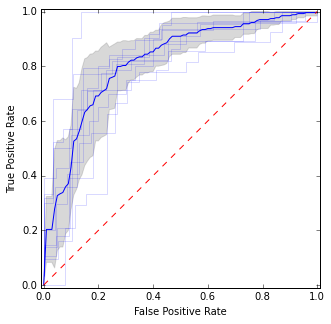
\includegraphics[width=2.5in]{fig/roc.png}&
{\small In this figure thick blue lines shows median performance seen in 10 machine learning
experiments, where each experiment learns on 90\% of the data (selected at random).
Note that  there is some variability seen in the thin blue lines, which are the
results from each individual trial. Comparing the median line to the rest,
we see that there is some variability of size $\epsilon$ in a learner's performance. }
\end{tabular}
\end{center}
\end{figure}

\section{Related Work}

confidence success. co_PIs have n=done much prior work in this area.

\subsection{inferface+ sandeep}

\subsection{Timm+ algorithms}

Researchers have proposed various solutions against adversarial machine learning attacks including
  \textit{adversarial training}, \textit{gradient masking}, \textit{defensive distillation}, and \textit{ensemble learning}. The idea of \textit{adversarial training}~\cite{DBLP:conf/iclr/TramerKPGBM18,DBLP:conf/iclr/NaKM18,DBLP:conf/iclr/MadryMSTV18,DBLP:conf/iclr/FarniaZT19,DBLP:conf/nips/ShafahiNG0DSDTG19,yin2019adversarial} is to build a ``golden'' dataset that ideally contains a set of curated attacks and normal data that are representative of the target system. The data is then used when training the model. Intuitively, if the model sees adversarial examples during training, its performance during prediction will be improved for adversarial examples generated in the same way. However, the problem with adversarial training is that it suffers from an optimized attack or adaptive attack, since this method only defends the model against the same attacks used to craft the examples originally included during training. 

\textit{Gradient masking}~\cite{papernot2018sok} is a technique that hides the model gradients to reduce model's sensitivity to adversarial examples. However, later work~\cite{DBLP:conf/icml/AthalyeC018} shows that even with gradient masking,
because of the transferability property of adversarial examples, the attackers can still build a substitute model and transfer the attacks.

\textit{Defensive distillation}~\cite{papernot2016distillation} tries to generate a new model whose gradients are much smaller than the original undefended model. If gradients are very small, some gradient-based attacks are no longer useful, as the attacker would need great distortions of the input data to achieve a sufficient change in the loss function. However, this method can be   ineffective~\cite{DBLP:journals/corr/CarliniW16} since, with a slight modification to a standard attack, attackers can still find adversarial examples on distilled networks.



Thr


Now consider tje
OMNI scores different hypermater configura
While exploring a large number of models (such as the trillions of options from \tbl{hyperparameters}), the ``expected model'' might be the one the scores
best across all the $y$-objectives. ; i.e. the optimal model from hyperparameter optimization, which is used in normal prediction. This model is the target of attackers and hence then becomes the victim model. Next, our optimizer surveys the hyperparameter space of models to find ``unexpected models''; i.e. models that are (a)~performing well (i.e., sub-optimal models) and (b)~dissimilar to the expected model (i.e., in the architecture). More specifically:
\bi
\item 
For hyperparameter optimization, we search a large space of possible configurations of a model to initialize a large \textit{model pool}.
\item
The {\em expected model} is a model from the model pool that performs best (under no attack). We call this model ``\textit{expected}'' since we conjecture that this model would be the target of an attacker, and becomes a victim model.
\item
We introduce an idea called \textit{model distance}, which is a numeric value indicating the degree of similarity of two models' hyperparameter configurations. A large model distance value means that two models are more likely to be different in their model architecture. 
\item The {\em unexpected models} are those whose performance within some small $\epsilon$ of the expected model but are more than some distance $t$ away from the expected model.   
\item
Those unexpected models are combined into a \textit{weighted ensemble}, in which each model $m_i$ in the ensemble with a weight $w_i$. The final prediction of this ensemble is the combined prediction of each model $m_i$ times its weight $w_i$. These weights are further optimized by an evolutionary algorithm that finds optimal $w_i$ setting that maximizes prediction performance.
\item
The final weighted ensemble, with its optimized weight setting is then deployed against evasion attacks.
\ei
  

Software security is often compared to the game ``whack-a-mole'' where players  wait for one or more  furry animals to poke their heads above ground, at which time you
try to ``whack'' them over the head with a large padded hammer before they escape. 

Vulnerability management is often compared to whac-a-mole, with new vulnerabilities appearing up constantly, and security teams realizing that they will eventually fall victim to an adversary. It is common to deprecate such an ad hoc whac-a-mole approach, arguing that security and adversarial defense requires a deep systems approach where the defenders institute long-term policies to (e.g.) deprecate the probability of vulnerabilities being added to a system in the first place.

But what if there was another way to runt the Whac-a-mole game? In our  approach, we turn the tables on adversial attachers 
by (a)~building a very large collection of different defnese algortms, then 
(b)~jumping between them at random at runtime. In this ``reversed Whac-a-mole game'', it is now the attackers
struggling to keep up with all the new tactic of the defenders.

Recent advances in nyperparameter optimziation (HPO) suggest that shis rppach is eindeed viable. As discusses in the next section, such optimziers explore two spaces:
(a)~the space of design decisions for a defnder and (b)~the space of design performance measures. In
standard HPO





of defense


Here, we propose to reverse the rules of that game. Adversarial security
learning is the process of an
external adversary learning examples that confusing internal defending
software
into concluding that some incoming
malicious data is actually benign.
recent results show that even
when the external attack does
not know the internal details,
they can still build a learner
show that an attacker can run a  machine learner ex when
the attackers do not know how
the defender learns to distnushish benign from malcisous inuput, 


A major contributing factor to this problem is that enterprise security teams are overwhelmed with tens of thousands of vulnerabilities across hundreds of thousands of assets that potentially need to be fixed. In an ideal world, you would whack all these moles systematically by “patching all” but this is impossible in most organizations. 




The NSF has spent hundreds of millions of dollars
on computational science software. When those projects fail and are ignored
(or fall into disrepute), then all those monies amount to little more than hard drives
gathering dust in some basement.  How can we find, and fix, faltering computational  science software (CSS)  projects
{\em before} they fail?
To answer this question, this proposal will   develop and certify and apply  the  {\IT} workbench (\underline{\bf M}easuring and mitigating  \underline{\bf U}nhealthy \underline{\bf S}cientific softwar\underline{\bf E}) to CSS software.
{\IT} will be an open source tool with ``hooks'' into source code repository systems such as Github.  {\IT} will distill decades
of work on software analytics into a form easily and rapidly usable by CSS projects. All the tools generated by this project will be placed on-line in a free-to-access Github repository and made available to the CSS community via an open source license.

A unique feature of this proposal is its scope. The software produced here will be applicable to  {\em any} CSS project using an open source repository (and we know at least 700 such projects). In our concept of operation, 
for any project  registered  with {\IT},
whenever developers commit code, they automatically receive an issue report commenting on the current and future health of their software, along with advice on how to improve that future state.  

That said, it is not enough to just advertise a service and expect others to use it. In this work,
NC State researchers will apply {\IT}   to as many CSS projects as possible. With  preliminary results in hand, they will approach CSS projects offering commentaries on their software (derived via our data miners)  and free consulting   on how to improve   projects. By  enticing CSS project members with results from their own projects, we anticipate growing a large user base amongst the CSS community.

\section{Goals}

Parts of {\IT} have been researched an developed for non-CSS software~\cite{peng2021defect,xia2019sequential,xia2020predicting,tu2020changing,tu2021mining}.
But before  we can assert that {\IT}  works on  CSS software, {\IT} needs to be
extend and improved and tested on CSS.
This proposal is a request for funding to perform the research and make the advances
needed to  optimizing  CSS
project corrective recommendations in order to:
\bi
\item {\em Minimize} the data collection required in order to make a recommendation;
\item
 {\em Minimize} the changes associated with {\IT}'s recommendations; 
\item
 {\em Maximize} the effect of {\IT}'s recommendations; 
\item
 {\em Maximize} the likelihood that CSS developers will actually apply those recommendations. 
\ei
% In order to avoid wasted development software effort
% this project will  build predictors for the   success or
% failure of a Computational Science Software (CSS) project. 
% Some CSS projects are more successful that others?
% Why? How early can we see if a project is going to be  more successful that others? If a project is flagging, how soon can we detect that? And
% how can that problem be   repaired? 

\begin{wrapfigure}{r}{3.2in}
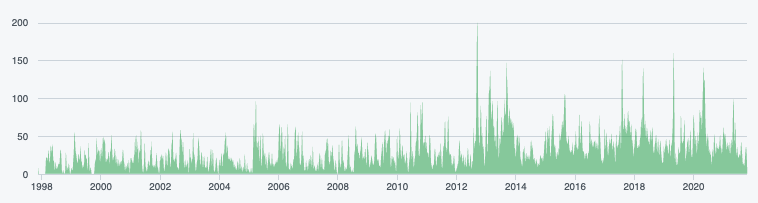
\includegraphics[width=3.2in]{fig/dealii.png}
\caption{Healthy CSS projects are   active. E.g. see the
numerous commits of new software to the deal.II    finite elements 
library since 1998. From  {\bf github.com/dealii}.}\label{fig:dealii}
\end{wrapfigure}
% ~{\IT} is a feasible goal. Our prior CSSI-funded work\footnote{Elements: Can Empirical SE be Adapted to Computational Science?
% Award \#1931425.  PI= Dr. Tim Menzies, NCState. 2019-2022.  }
% has shown regularities in CSS software that,
% in theory, make it amenable to  accurate prediction and repair.  
% When some phenomenon is regular and predictable then it makes it a clear candidate
% for control strategies. Hence this proposal. 
Central to this proposal is the concept of ``project health''.
Researchers agree that ``healthy'' software projects are   ``vigorous'' and ``active''~\cite{han2019characterization, wahyudin2007monitoring,jansen2014measuring,manikas2013reviewing,link2018assessing,wynn2007assessing,crowston2006assessing}. 
For example,   the 
deal.II  adaptive finite elements package  is very 
``healthy''
since,  at the time of this writing,
it  has over 10,000 closed ``pull requests'' (where people
outside the core team have successfully contributed fixes or enhancements).
Another measure of the ``health'' of that deal.ii is that it receives
thousands of commits (changes to its software) each year (see \fig{dealii}).




For non-CSS   software,
PI Menzies and his students 
(Mr. Taianpei Xia~\cite{xia2019sequential,xia2020predicting} and Mr. Huy Tu~\cite{tu2020changing,tu2021mining})
have used early prototypes of {\IT} to successful predicted project ``health''  twenty four months into the future. As discussed below, such information can be used to guide project improvement plans (e.g. improvement planning may be not be required, when a project is predicted to be healthy for the foreseeable future.

That said, those predictions have only be performed on conventional software (i.e. not CSS software). 
As discussed in
\S\ref{prior},
 CSS software  is very different to conventional software. E.g. the latter is subject to the whims of market forces while the former is subject to whims of  funding
agencies. Also, CSS developers are specialists in physics, chemistry, etc and so may lack certain training and experience of SE methods. 
 Accordingly, prior success for predicting health on conventional software needs to be checked for CSS software. Hence our first goal is:
\begin{formal}\noindent
{\bf Goal1}  predict project health for  some CSS projects (discussed in \S\ref{goal1}).
\end{formal}
\noindent
Merely measuring a problem is insufficient. After 
{\em measuring} must come {\em mitigation}. Once
we can  recognize a failing project, the next
step is to seek ways to fix it.
PI Menzies (and his graduate
student Mr. Kewen Peng~\cite{peng2021defect})
have shown that   software can be trusted to decrease its defects and increase its health. Since  this approach has  yet to tested on CSS software, our next goal must be: 
\begin{formal}\noindent
 {\bf Goal2}  plan effective improvements for some  CSS projects (discussed in \S\ref{goal2}).
\end{formal}





% \begin{wrapfigure}{r}{2.5in}
% 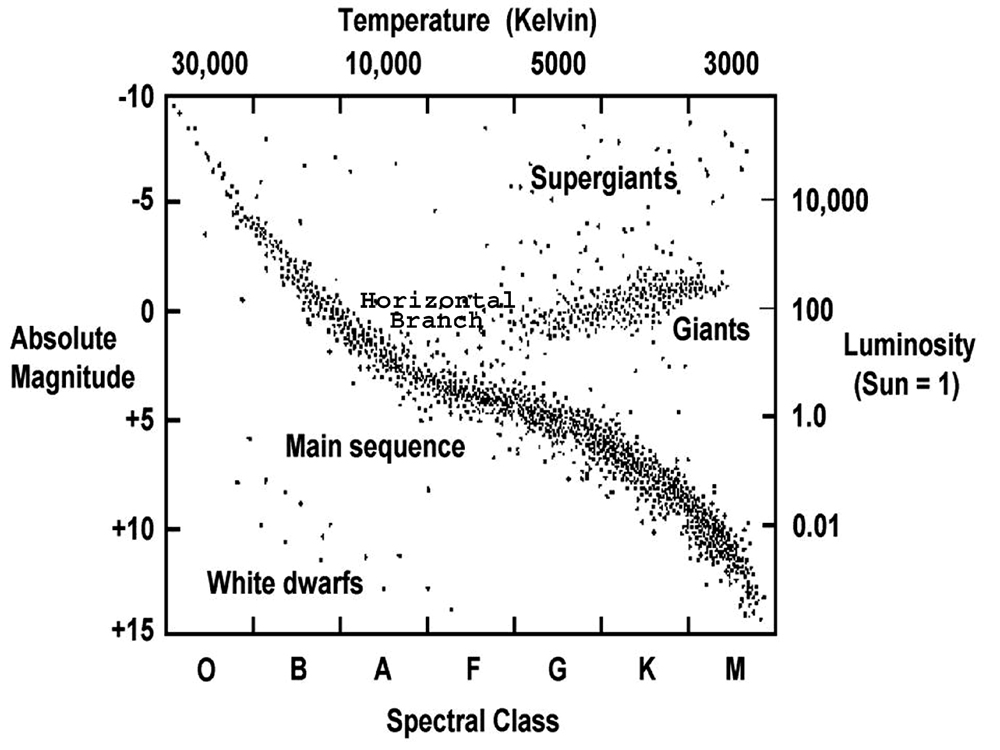
\includegraphics[width=2.5in]{fig/mainsequence.png}
% \caption{ Astronomers use  Hertzsprung-Russell diagrams to determine where is a star within the overall life-cycle of all stars.   Can we do something similar with software systems?}\label{fig:hr}
% \end{wrapfigure}
% By measuring, then mitigating, problems  in CSS software, this project will  enable all the 
% science that is discovered by that software.   Researchers into software
% analytics claim that there exists  
%   properties within all software projects that allows for the prediction
% of the future state of those projects. Like atoms in a star, these
% properties might be highly variable within any local context. 
% Nevertheless, if we step back to see the bigger picture, a pattern can emerge; e.g. see 
% Hertzsprung-Russell diagram of \fig{hr}. As with atoms, so too with software developers, If  we step back from the specifics of individual
% components, we can make predictions about large systems of individual developers.
%  But unlike stellar evolution,
% using the methods of this paper, developers and funding agencies can not only  predict 
% the current
% expected fate of a software project,  they can also take steps to 
% {\em change that fate}.

% % This project is somewhat different to a standard CSSI project. 
% % Instead of making predictions about physical phenomena,
% % in this work, we step back from that as say our ``phenomena''
% % being studied is the act of software development itself:

% % \begin{center}
% % {\em 
% % This proposal will make predictions about the   
% % process that  makes the software that enables computational science. 
% % \end{center}



% On the other hand,
% some CSS projects are not healthy and are ignored by the community
% (as witnessed by very little vigor or activity). To find, then fix,
% such projects, we apply methods from open source software to CSS projects.
% Those methods build models that offer
% accurate predictions on open source software project health,3,6,12,24 months into the future
% (where ``health'' is measured by values like number of closed pull requests and number of contributors).
% Those      methods have only been tested on software 
% that is ``market-driven''  (e.g. by   open source Silicon Valley industries) rather than ``science-driven''
% (e.g. by NSF funding cycles). Hence, here, we must test them   on computational science projects:
% \begin{formal}\noindent
% {\bf Goal1} of this project is to see how widely these health prediction methods apply to CSS projects.\newline
%  {\bf Goal2} of this project is to see if our predictors can be used to drive planners that propose
% useful changes to projects (where ``useful'' means ``improve project health'').
% \end{formal}
\noindent
Given the size of the CSS  community, our project improvement  goals
are  only widely applicable
if we can tame the data collection cost associated with this kind of analysis.  Outside of CSS
software,
{\em semi-supervised learning} has been used
to  restrain data collection to just the most informative examples. For non-CSS projects this
has meant  the effort associated with this kind of
study can be reduced by a factor of 40~\cite{tu2021frugal}\footnote{A core problem with analytics is ``labelling''; i.e. acquiring the ground truth associated with each example. Semi-supervised methods take a small number of labels then intelligently ``spread them round'' their nearest neighbors. In this way, Tu et al.~\cite{tu2021frugal} was able to reduce the labelling effort of their case study to just 2.5\% of the examples.}. 
But the value of that semi-supervised learning to
to CSS projects
has yet to be tested. Hence:
\begin{formal}\noindent
{\bf Goal3}: achieve Goal1,Goal2 for CSS projects via minimal data collection (discussed in \S\ref{goal3}).
\end{formal}
\noindent
Moving on to our next goal,
all this  research is   wasted {\em unless} it is applied
within the CSS community. Accordingly, our next goal must be:

\begin{formal}\noindent
{\bf Goal4}:  get our recommendations used by CSS community (discussed in \S\ref{goal4}).
\end{formal}
\noindent
For reasons of data availability, this proposal deals with CSS projects stored in the Github code repository.
By our counts, there are at least 700 such projects. But what about
other kinds of software?
\begin{formal}\noindent
  {\bf Goal5}:  apply our methods to CSS projects not stored in Github
  (discussed in \S\ref{goal5}).
\end{formal}
\noindent
Finally, we need one last goal:
\begin{formal}\noindent
 {\bf Goal6}:
find a set of general methods   for improving CSS projects (discussed in \S\ref{goal6}).
\end{formal}
\noindent
Technically speaking, {\bf Goal6} is a 
{\em transfer learning task}~\cite{KrishnaMF16,Nam13,Ma2012,jing15,Kocaguneli2014,yu2017feature,jamshidi2017transfer,pan2009survey,qing2015cross,li2018cost};
i.e.   lessons from one kind of project are   transferred
to another. 
As discussed in 
\S\ref{mm}, recently we had much success with hierarchical clustering algorithms that generate a handful of models  that apply to hundreds of conventional projects~\cite{majumder2019learning}. In  this proposal,
we would check if those methods work for CSS projects.
 
% The experience to date (with standard open source software~\cite{xia2020predicting}) is that while the prediction models are local to each project,    the method used to generate those models works for multiple projects.  That said, as discussed below, there is reason to suspect that it might be possible
% that CSS software is more regular that standard open source source. This means that it might be possible to learn general lessons for project health that apply to many CSS projects both within and without Github.
 
 
\section{Background}
\subsection{Frequently Asked Questions}
\noindent
 When discussing this proposal with colleagues, their first question is always:
 
 \begin{center}
 {\em FAQ1: are we trying to replace research scientists as they apply their creativity to computational science problems?} 
 \end{center} That is not the goal here.
 Instead,  {\IT} will explore  the software engineering decisions that can lead to
project success or failure.
 When we look at success stories for community-developed   software
 (e.g. the Apache Foundation or the Linux Foundation~\cite{apacheprojects,linuxprojects}), we find that the most successful software  projects
 are those  that attract  
 a large user base
 {\em and} a large funding base (where 3rd parties offer support for that code). While
 the funding support any one source   may be small,
 the combined funding   enables  the infrastructure needed for long-term viability.
 
 When attracting a funding base for a project,   the {\em reputation} of that project is very important. No one wants to fund a flailing or failing project. Hence,
 project health is often used to make the case 
 (e.g. to upper-management) that  some   software is worthy of funding.
A similar story can be told about how
 to attract developers to user your tools~\cite{xia21}. No
 one wants to based their work on some library
 that, in the near future, will be abandoned by its
 developers.  Perceptions of future  project health  of a project determines how many developers will be attracted to a project.
 
 Note that in both cases,   improving project health (via the methods of this proposal)  increases
 the probability that a project will become more sustainable (by attracting more
 funding and more developers).
  

Another questions we are often asked is:

\begin{center}
{\em FAQ2: what can be changed in a software project to make it better?}
\end{center}
Decades of research into software analytics by PI Menzies~\cite{menzies2016perspectives,menzies2018software,bird2015art,xia2019sequential,xia2020predicting,tu2020changing,tu2021mining,peng2021defect},
and others~\cite{kim2016emerging,buse2012information,amershi2019software,barry1981software}, shows that there are many  software project decisions that can make a project more (or less) attractive to other developers:
Some of these reasons are high-level
e.g.
\bi
\item
Choice of platform; using/avoiding unpopular dependencies; how the project interacts with the scientific developer community; choice of software license; numerous internal
architectural decisions; etc. 
\ei
Some of these reasons are much lower level; e.g.
\bi
\item
If a specific application programmer's interface
is tedious or complex to use, then external developers
will avoid this API, and perhaps even this entire CSS project.
\ei
In either case (low-level or high-level issues), {\IT}
will employ data mining on project data to:
\bi
\item Recognize a problem; e.g. recognize when the comments about an API are mostly negative;
\item
Propose a solution; e.g. recommend that the API be simplified.
\ei
Finally, we are often asked: 

\begin{center}{\em FAQ3: if {\IT} has already been developed, what is the core science of the problem being discussed here?}
\end{center}
In reply we say that parts of
{\IT} have only been tested only on general open source software, not CSS software. As discussed
below, these two kinds of software
are different enough to make it an open question if
{\IT} will work for CSS. 

As to the question about core science,
while {\bf Goal1, Goal4, Goal5} are case studies (where we apply  old {\IT} to new data), 
the other goals address core scientific issues
 relevant for any data mining problem:
 \bi
 \item {\bf Goal2}: Can our learners make any predictions about what to change in order to alter future outcomes?
\item {\bf Goal3}: Can we reduce the data sampling needed
to build an adequate model?
\item {\bf Goal6}: How general are our models (or must  we always reason over numerous different   models)?
\ei
\newpage
\subsection{Definitions}\label{distinct}
\noindent
Our premise is that Computational Science Software projects (CSS)
is very   
different to standard open source software (SOSS).
Hence, even thought we have preliminary results with {\IT} on SOSS code,
we can not assert that {\IT} will work on CSS software until we test it.

The next section offer empirical data on the   differences between CSS and SOSS. Before that, we offer some definitions:
\bi
\item {\em SOSS software:} 
Conventional open-source projects are developed and distributed
for free redistribution~\cite{Raja12}. SOSS tools are widely used, even within the CSS community.
For our purposes, the major different between CSS and SOSS is the level of domain comprehension
seen in the developers.  While CSS developers have a deep understanding of the phenomena that
are explored, an SOSS developer can be anyone in the world with any level of domain training.

\item {\em CSS software:} Computational scientists explore software models than  
explore the physical effects. Exploring such models can be  faster, cheaper, and safer than exploring
the real world. For example, it is safer to explore models of hurricanes rather than the real thing.
For another example,
in material science, CSS explores the properties of new materials by
synthesizing them. Such synthesis can be very  expensive so standard practice
is to use software to cull the space of possibilities (e.g. via a finite
element analysis).  
A key feature of CSS software is that extensive background needed to understand, maintain and improve
this kind of software. For this reason, many CSS developers have advanced degrees in Physics, Chemistry, etc.  
Another difference is that 
 CSS code is developed more for science reasons rather than,  in the case of SOSS, to satisfy they whims of the developers or the vagaries
of the market place.
\ei


% While all this will be applied to computational science, the more general   point here is
% a comment on how huamns should investigate the work.  
% Brieman decribes two cluterures of statiscal anaysis of data: either assume an  apriori some distribution (and go hunt for it) or apply some open-ended data mining  method that hunts though a large space of possible
% models before decising which one might be approrpaite. It is an open 
% isse which approach is most prdocutive. Both approaches
% have their
% ardent supporters and detractors (e.g. the Google team lead by Norvig endorses ``open-ended''
% while Bayesians urge us to first define our apriori assumptions before doing any mining).
% This NSF proposal 





%XXXX bridge from here to other stuff 
\subsection{Results from Prior CSSI Projects}\label{prior}


The   section offers  empirical evidence
that CSS projects are fundamentally different to
SOSS projects.  These results come from a  prior  CSSI-funded    project\footnote{Elements: Can Empirical SE be Adapted to Computational Science?
Award \#1931425.  PI= Dr. Tim Menzies, NCState. 2019-2022.}.  The differences documented
in this section justify the core premise of this work: even if parts of {\IT} are known to work for standard software systems, we still need to check if it works for CSS code. 


 \begin{wraptable}{r}{1.5in}
\vspace{-5pt}
\centering
\caption{Project selection rules. From~\cite{Kalliamvakou:2014}.}\label{tbl:sanity}
\vspace{-5pt}
\footnotesize
\begin{tabular}{r|l}
 Check   & Condition    \\\hline
 \# Developers & $\geq$ 7 \\
 Pull requests  & $>$ 0 \\
Issues & $>$ 10 \\
Releases &  $>$ 1 \\
Commits & $>$ 20 \\
Duration  & $>$ 1 year 
\end{tabular}%}
\vspace{-10pt}
\end{wraptable} 
The following  study used (1)~a
 {\bf comparison set} of CSS and SOSS projects;
 (2)~a set of 
 {\bf project health indicators}.
In this   study, we
 compared 60 CSS projects to  1037 Github SOSS projects from~\cite{Majumder19}.
 We  use  project data from Github since this keeps data on CSS and both SOSS in a standardized way.
 
As to how we selected these SOSS projects,
the software analytics community
has long debated how to select ``interesting'' projects. Their standard ``sanity checks'' (used in this analysis) are shown in 
Table~\ref{tbl:sanity}.

As to our selection of CSS projects, 
we combined projects associated with a specific NSF grant and from   contacts in the CSS community
(from the Molecular Sciences Software Institute (MOLSSI) and the Science Gateways Community Institute (SGCI)).
Many of these were single-person projects (e.g.   ``glue'' projects from the Gateway). While those kinds of projects are an important part of the CSS community, in terms of number of developers, we find that that we can cover far more developers by applying the Table~\ref{tbl:sanity} sanity checks to that sample of CSS projects.
 

  These CSS and SOSS projects were compared using the following   health indicators:
\be
\item \textit{Developers}: are the active contributors to a project.
% , who code and submit their code using commit to the code base. The number of developers signifies the interest of developers in actively participating in the project and volume of the work.
  
  

\item \textit{Commits:} adds the latest source code to the repository.
% in version control systems, a commit adds the latest changes to the source code to the repository, making these changes part of the head revision of the repository. 

\item  \textit{Open \& Closed Issues:} are used to track ideas, enhancements, tasks, or bugs.

% users and developers of a repository on Github use issues as a place to track ideas, enhancements, tasks, or bugs. As they work, they open issues with Github. When developers address those matters, they close the issues.

\item  \textit{Tags}: are references that point to a specific time in the Git version control history. 
%Tagging is generally used for marking version release (i.e., v1.0.1).


\item  \textit{Releases:} are different versions published (and  signifies a considerable  change between each version)
% mark a specific point in the repository’s history. The number of releases defines different versions published (and  signifies a considerable  change between each version).

\item \textit{Duration:} length of the project from its inception to the current date or project archive date (in weeks).
%of a project marks the length of the project from its inception to the current date or project archive date (in week as a unit of time). It signifies how long a project has been running and in the active development phase.
\item \textit{Stars:}  people who
  ``liked'' a project's repository (and bookmarked it to get updates on   future progress.)
  
\item   \textit{Forks}: how many people are interested in the repository to make a copy of it while  allowing users to freely experiment without affecting the original project.
   
   % Forking a repository allows users to freely experiment with changes without affecting the original project. 
   % This number is an indicator of how many people are interested in the repository and actively thinking of modification of the original version.
  
\item   \textit{Watchers}:  Github users asking to be notified of repository activity, but have not become collaborators. 
   % This is a representative of people actively monitoring projects, because of possible interest or dependency.
\ee
Note that some of these indicators are more insightful than others. ``Stars'', for example, is more a popularity contest than a deep semantic dive into a system. On the other hand, ``number of closed issues'' is a core measure  revealing who cares enough about   code to recompile it and fight with its errors.
 
 
% \begin{wraptable}{r}{1.5in}
% \vspace{-15pt}
% \caption{Languages in 59 CSc projects.  
% }\label{tbl:language}
% \vspace{-12pt}
%  \footnotesize
% %\begin{threeparttable}
% %\vspace{-10pt}
% %\resizebox{!}{0.2\linewidth}{
% %\setlength        abcolsep{10pt}
%  \hspace{-3pt}\begin{tabular}{l|c|c}
%  \multicolumn{1}{c|}{} & \multicolumn{1}{c|}{Count} & \multicolumn{1}{c}{Percent}\\
% \hline
% Other & 3 &  5\%  \\ 
% Javascript	& 2 & 3\% \\ 
% C &	3 & 5\% \\ 
% Java	& 5 & 9\% \\ 
% Fortran	& 6 & 10\% \\
% C++	& 17 & 29\% \\
% Python & 23 & 39\% 
% \end{tabular}
% \vspace{-10pt}
% %}
% %\end{threeparttable}
% \end{wraptable}
\fig{health} compares these indicators for CSS and SOSS projects.
 Based on  a combination of
  a 95\% confidence bootstrap statistical test~\cite{efron94} and an A12 effect size test~\cite{arcuri2011practical}, we offer the following notes:
  \bi
  \item Both projects have similar number of
  developers per project;
  \item
CSS  projects have a shorter  median {\em duration} 
than SOSS projects   (281 weeks versus 409 weeks);
\item Interestingly, in that time, the CSS projects
  (a)~make more commits and (b)~close many more issues and (c)~make many more releases.
  \item
  That is to say, at least in this sample, CSS projects
complete more work with the same number of people in 
signficantly less time than    SOSS projects.
  \ei 
\begin{figure}[!b]
~~~~~~~~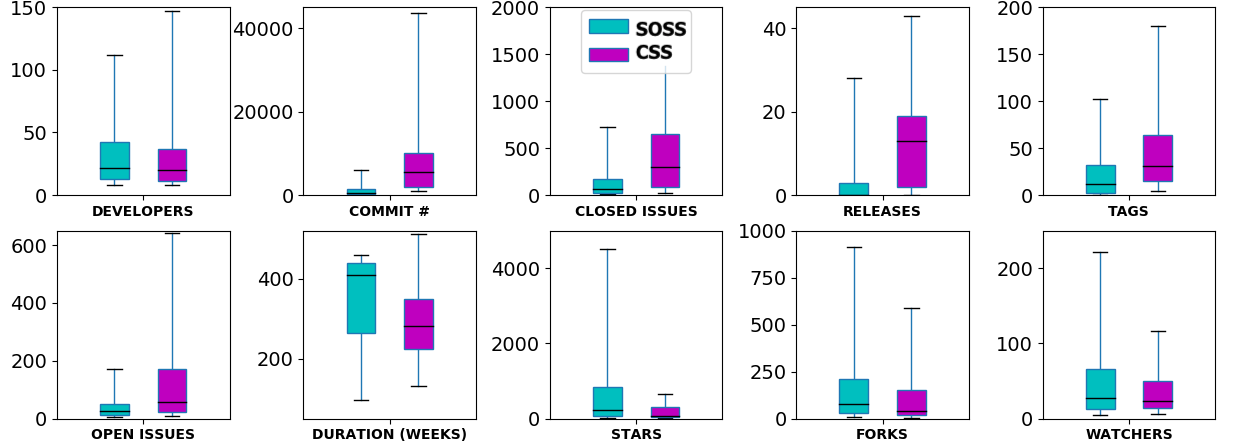
\includegraphics[width=5.7in]{fig/compare.png}
\caption{
Standard open source projects are shown in turquoise

\includegraphics[height=2mm,width=5mm]{fig/SOSS.png}.
Computational science software projects are shown in  purple

\includegraphics[height=2mm,width=5mm]{fig/CSS.png}.
 By all these health indicators, the following
CSS projects are better than SOSS:
{\em ABINIT,
AMBER,
APBS,
BLIS,
GooFit,
HooMD-blue,
LAMMPS,
LIBMESH,
Luigi,
MADNESS,
MDAnalysis,
MPQC,
NWChem,
OpenMPI,
OpenMX,
OpenMm,
PCMSolver,
PLUMED,
Psi4,
RMG-Py,
SCIRun,
TRILINOS,
TauDEM,
Use,
Xenon,
abaco,
cctools,
changa,
cyclus,
dealii,
elasticsearch,
forcebalance,
foyer,
hydroshare,
irods,
learnsphere,
mast,
mdtraj,
metpy,
openforcefield,
openmmtools,
orca,
parsl,
pymatgen,
pyscf,
quantum\_package,
radical-pilot,
signac,
signac-flow,
trellis,
yank,
yt}.
}\label{fig:health}
\end{figure}
% \fig{health} is not our only evidence that of the robust
% health of many CSS software. Many writers
% such as  Basili, and others~\cite{basili08_hpc, carver07_environment, Prabhu11_cssurvey, kendall05_C, ragan14_pythoncs,faulk09_secs,sanders08_risk,Prabhu11_cssurvey} express are concerned that CSS projects
% are using older tools (Fortran is often mentioned).
% To test if CSS software is  using out-moded tools, we counted  what were the main languages in our CSS sample.
% This test assumes that if CSS teams are mostly focused on ``old'' technology then most of those projects would use ``old'' languages and would not use automated testing
% tools such as  Travis CI\footnote{Travis
% CI is an automatic testing facility that is often run from Github.
% From {\em Wikidpedia}: When Travis CI has been activated for a given repository, GitHub will notify it whenever new commits are pushed to that repository or a pull request is submitted.  Travis CI will then check out the relevant branch and run the commands specified in the  .travis.yml file, which usually build the software and run any automated tests. When that process has completed, Travis notifies the developer(s).}
% The results of this ``are they using newer technology?'' test are shown in \tbl{language}.
% As seen there,  C and Fortran are just 15\% of our sample.
% Even if we call C++ ``old''\footnote{
% Johanson et al.~\cite{johan18_secs} say that, in CSS, Fortran and C are examples of this ``old'' technology. The use of C++ is an interesting borderline case- Johanson et al. regard that as ``new technology'' even though it is now decades old. In any case, C++ is not a part of the \fig{language} results.}, then the ``older'' technologies of \tnl{language}
% cover less than half the sample (44\%).
% As to other measures of ``new'', we find that  $43/59=73\%$
% have active
% Travis CI connections. 
% %We also observe some other SE methods and technologies include \textit{YT}~\cite{yt_project} and  \textit{AMBER}~\cite{Amber-MD} employ Docker~\cite{DOCKER} to simplify applications deployment,  \textit{LAMMPS}~\cite{lammps-sandia} and \textit{DEALII}~\cite{BangerthHartmannKanschat2007} can run on parallel processors, \textit{PSI4}~\cite{psi4} and \textit{XENON}~\cite{xenon} to test   code coverage. 
One way to summarize the above is that:
 
 
  \begin{center}
  {\em Computational science projects are performing much  better than standard SOSS
projects.} 
  \end{center}
This result is at odds with  prior work~\cite{basili08_hpc, carver07_environment, Prabhu11_cssurvey, kendall05_C, ragan14_pythoncs,segal_enduser,  carver13_perception, sanders08_risk} that complains that  CSS software is somehow
problematic:
\bi
\item
Basili et al., and others~\cite{basili08_hpc, carver07_environment, Prabhu11_cssurvey, kendall05_C, ragan14_pythoncs} say that
computational scientists prefer
``older''-style programming languages and technologies (and disregard most of the newer SE methods). To that, we would reply that even if they are using supposedly older tools, 
\fig{health} suggests CSS developers are using those tools very effectively. 
\item
Segal~\cite{segal_enduser},
and others~\cite{basili08_hpc, carver13_perception, sanders08_risk} comment that  few CSS scientists are trained in SE.  This is concerning as a lack of training might lead to sub-optimal software
development
 (for many of these people,
learning SE is perceived as an excessive additional burden~\cite{boyle09_lessons}).
To this concern we would reply that however they are trained, 
\fig{health} suggests that CSS developers are
using that training very effectively.
\ei
% % Before we list those widely-held beliefs, we stress that our research
% % suggests that the following beliefs
% % are \underline{\bf NOT} true (at least, for the CSS software we examined in Github):
% % \bi
% % \item
% % {\em Belief1: CSS developers have
% % old tools.}
% % According to this belief, CSS software uses old,
% % and possibly sub-optimal and out-dated, methods.
% % For example,
% % The usual argument here is that CSc Scientists are skeptical of modern SE methods and new technologies/languages.
% % This is based on several factors such as
% % (a)~a prejudice against  newer languages;
% % (b)~a perception that CSS developers would not 
% %   find new tools very  useful~\cite{Prabhu11_cssurvey};
% %   (c)~a decades-long commitment to  older-style languages (Fortran \& C)~\cite{faulk09_secs}.
% % (d)~a  belief that the extra features of the newer languages needlessly conflate functionality that can be more easily implemented in, e.g., one line of ``C'' macros~\cite{sanders08_risk}; 
% % \item
% % {\em Belief2: CSS developers have  the wrong skills,
% % and may not even want to learn new ones.}
% % CSS software is worse that other
% % code, it is said,  since it is built
% % by people not trained in up-to-date methods.
% % For example,   
% \ei
% Neither of these beliefs are supported by our results.
% The discussion around \tbl{language} found not evidence of a preponderance of older technology. Further,
% the results of \fig{health}, CSS projects are delivering and maintaining more software in less time with fewer developers than SOSS projects. 
To explain this discrepancy between
the optimism of \fig{health}
and the pessimism of Segal, Basili
and others~\cite{basili08_hpc, carver07_environment, Prabhu11_cssurvey, kendall05_C, ragan14_pythoncs,segal_enduser,  carver13_perception, sanders08_risk}, 
we offer three notes:\bi
\item
Software development is certainly difficult.
Hence, Segal, Basili
and others are certainly correct in warning the CSS software development is difficult. That said,
by asking a slightly different question, we arrive a new perspective not previously reported. Instead of asking
``Q1) is CSS code development difficult?'', we   ask instead ``Q2) is CSS code development
{\em comparatively more difficult} than
other kinds of software?''. And as \fig{health} shows us, the answer to Q2 is ``no''.
\item
Most of the papers lamenting the state of CSS code come from before the recent Silicon Valley boom. In our recent discussions with postdocs and Ph.D. students working on CSS projects,
we found that these developers were well aware of the potential salaries if they are adept at the popular tools used by contemporary agile software companies.
Hence we suggest that something of a ``phase change'' has come over
CSS software and that newer codes should be expected to be somewhat more
better than past offerings.
\item
When computational scientists developers write CSS code, they are exploring domains with  an extensive background theory (all the physics and chemistry achieved in thousands of years of scientific research).  When other developers write code
about (e.g.) database systems, they are writing about domains with only a few decades
of theory.  Also, CSS developers typically have multiple degrees, some even with higher degrees. Conventional software authors, on the other hand, many have a far less
scientific training. When stated this way, it is hardly surprising that developers with more scientific working over a  richer background theory generate better systems than otherwise.
\ei
\subsection{Measuring and Mitigating Project Health Issues}\label{mm}
 \begin{wraptable}{r}{3in}
 \begin{adjustbox}{max width=3in}
 \begin{tabular}{l|rrrrrr}
\multicolumn{7}{c}{ error =  MRE =  $\mathit{abs}(\mathit{predicted} - \mathit{actual})/\mathit{actual}$ (so {\em less} is {\em better})   }\\\hline
\rowcolor[HTML]{ECF4FF} 

{\cellcolor[HTML]{FFFFFF} predicting for:} & {\color[HTML]{000000} KNN} & {\color[HTML]{000000} LNR} & {\color[HTML]{000000} SVR} & {\color[HTML]{000000} RF} & {\color[HTML]{000000} CART} & {\color[HTML]{000000} DECART} \\\hline
{\color[HTML]{000000}   \#commits} & \cellcolor[HTML]{E2E2E2}53\% & \cellcolor[HTML]{F3F3F3}107\% & \cellcolor[HTML]{E9E9E9}68\% & \cellcolor[HTML]{E1E1E1}53\% & \cellcolor[HTML]{E2E2E2}52\% & \cellcolor[HTML]{DCDCDC}41\% \\
{\color[HTML]{000000}   \#contributors} & \cellcolor[HTML]{CACACA}32\% & \cellcolor[HTML]{9F9F9F}26\% & \cellcolor[HTML]{D9D9D9}35\% & \cellcolor[HTML]{898989}24\% & \cellcolor[HTML]{989898}24\% & \cellcolor[HTML]{666666}\textcolor{white}{18\%} \\
{\color[HTML]{000000}    \#stars} & \cellcolor[HTML]{BFBFBF}30\% & \cellcolor[HTML]{D9D9D9}35\% & \cellcolor[HTML]{D9D9D9}36\% & \cellcolor[HTML]{B9B9B9}30\% & \cellcolor[HTML]{DADADA}37\% & \cellcolor[HTML]{9F9F9F}26\% \\
{\color[HTML]{000000}  \#open issues} & \cellcolor[HTML]{D9D9D9}36\% & \cellcolor[HTML]{DEDEDE}45\% & \cellcolor[HTML]{DBDBDB}39\% & \cellcolor[HTML]{D9D9D9}34\% & \cellcolor[HTML]{C3C3C3}31\% & \cellcolor[HTML]{8C8C8C}23\% \\
{\color[HTML]{000000}   \#closed issues} & \cellcolor[HTML]{DCDCDC}41\% & \cellcolor[HTML]{B5B5B5}29\% & \cellcolor[HTML]{DDDDDD}44\% & \cellcolor[HTML]{ADADAD}28\% & \cellcolor[HTML]{CACACA}32\% & \cellcolor[HTML]{828282}22\% \\
{\color[HTML]{000000}   \#closed pull requests} & \cellcolor[HTML]{DADADA}38\% & \cellcolor[HTML]{DBDBDB}39\% & \cellcolor[HTML]{DBDBDB}40\% & \cellcolor[HTML]{DEDEDE}44\% & \cellcolor[HTML]{DCDCDC}41\% & \cellcolor[HTML]{C3C3C3}31\%
\end{tabular} 
\end{adjustbox}   
\caption{Predicting project health. Median errors  in  1,159 SOSS projects~\cite{xia2020predicting}.  Darker cells=less
error. 
Lowest errors from ``DECART''. }\label{tbl:med_mre}
\end{wraptable}
Software development can be hard. Even if \fig{health} shows that CSS projects
might be relatively stronger than SOSS projects, there are still all-to-many examples
of NSF-funded CSSI projects that failed, or fell into disrepute, or have been ignored
by the rest of the community.
To fix that problem this section describes  methods to {\em find}, then {\em fix}
a failing project. 

Just to be clear, {\em none} of the material in this section
have yet been applied to CSS projects. The methods of this section would need 
significant extension to achieve the goals listed in the introduction. In the {\em next} section  of this proposal,
we addresses how we would test, then adapt,
these methods for CSS projects.
 
PI Menzies' prior work with generating health predictors (for non-CSS software)
was reported in~\cite{xia2019sequential,xia2020predicting}. 
In that report it was noted that numerous research had studied
project health~\cite{jansen2014measuring,manikas2013reviewing,chaoss,weber2014makes,borges2016predicting,wang2018will,bao2019large,kikas2016using,jarczyk2018surgical,qi2017software,chen2014predicting}. PI Menzies found numerous shortcomings with that
prior work:
\bi
\item That prior work usually studied a very small number of projects (perhaps, just even one);
\item That prior work usually explored a small number of indicators
(often, only one);
\item That prior work did not explore a range of learner methods;
\item That prior work did not apply tuning methods to automatically infer the best learner control parameters.
\ei
% For example,
% the CART regression tree learner has hyperparameters:
% \bi
% \item 
% max\_features: number of features to consider when looking for the best split;
% \item 
% max\_depth:   maximum depth of the learned tree;
% \item 
% min\-sample-leaf: minimum samples required to be at a leaf node
% \item
% min\_sample\_split: minimum samples required to split internal node
% \ei
 







~To address those issues, PI Menzies (and his student
Mr. Tianpei  Xia) applied their DECART tool to a wide range 
of projects~\cite{xia2020predicting}. DECART is  a recursive entropy learner 
tuned by 
a hyperparameter optimizer~\cite{storn1997differential}. PI Menzies tested DECART on
1100+ Gitub projects to
explore seven health indicators. In the study,
DECART was compared to five different learners (linear regression, CART, random forests, k-nearest neighbor, and support vector regression). It was found that:
\bi
\item
The right-hand-side column of  \tbl{med_mre}  
shows that DECART's errors
($abs(want\;-\;got)/want$)
are much lower than the other studied methods.
 These results     are 
 unexpectedly accurate.
Prior experiment with effort estimation had generated predictions
 with error ranging up to 200\%~\cite{kocaguneli2012value}.
 Hence our  pre-experimental expectation was that  these
 prediction errors would be up to ten times larger than what is seen in the right-hand-side
 column of \tbl{med_mre}.
\item
We have repeated the \tbl{med_mre} analysis for predictions up to two years into the futre.
The prediction error was observed to increase, but not by very much  (as little as 5 to 10\% more).
\ei
In summary,   these predictions are hence accurate enough to predict medium-term trends in a project (at
least for the SOSS projects studied here).  
 
\definecolor{aoenglish}{rgb}{0.0, 0.5, 0.0}
 \definecolor{applegreen}{rgb}{0.74, 0.85, 0.75}


That said, \tbl{med_mre} is more a 
{\em starting point} than a {\em conclusion}.
All these results are from SOSS project so,
without further testing,
it is unclear if these methods   work on CSS projects.
Also,   once we can predict for  $X$,
then the next question to ask is 
``how can we improve $X$''?  

To address that issue for (non-CSS) projects, PI Menzies
and his student Mr. Kewen Peng made several  observations~\cite{peng2021defect}.
 {\bf FIRSTLY}, the delta $\Delta$
between two regions of the data is
a candidate {\em plan} for moving from
more region to another. For example, consider the defect prediction
regression tree of \fig{XTREE}.
Each branch of that tree a logical conjunction.
To create a plan that changes a project from
(e.g.) a defective 
  \textcolor{orange}{{\bf current branch}}  to a better
 \textcolor{aoenglish}{{\bf desired branch}}, we can apply the 
$\Delta$ between the two branches. In the case of the example of
\fig{XTREE}, plan is to   minimize two static code attributes {\em lcom} and {\em cam}.  Such values can be changed via {\em software refactoring operators}
such as ``fold a sub-class into a superclass''; or ``push down a super-class method into 
the children''.



{\bf SECONDLY},  the models generated  by DECART (that lead to  \tbl{med_mre}) are of the same  form as \fig{XTREE}.
\begin{wrapfigure}{r}{3in}
   \includegraphics[width=3in]{fig/XTREE_samp.pdf} 
    \caption{  A {\em plan}
     is the delta $\Delta$
     that moves a project from the defective  \textcolor{orange}{{\bf current branch}}
    (where defect probability  is 1.00)  to another
     \textcolor{aoenglish}{{\bf desired branch}} (with zero defects).}
    \label{fig:XTREE}
\end{wrapfigure}
That, is DECART could be a front-end to a project planning process.
Note that
this  planning process that could be applied to    any model that comments on projects process or project attributes that tend towards  better/worst results (i.e. to more than merely the static code attributes of \fig{XTREE}).
 
 




~{\bf THIRDLY},   it is important to check the plans found in this way. Such plans  are hardly causal determinants of behaviour  
(causality is  precisely defined--    a single counterexample can refute the causal claim~\cite{AAAI_1990}). 
These  plans  have some likelihood (but no certainty) that they will work in the
way predicted for future projects. Hence, this kind of plan generation has to be paired with some {\em sanity check}
that prunes bad plans. 
Accordingly,
Menzies and Peng~\cite{peng2021defect}
used a {\em precedence sanity check} to only endorse  plans that proposed changes found in the historical record of a project. They found
that plans found in this way were much smaller than those proposed
by prior state-of-the-art mechanisms;
and just as effective (and sometimes better) than that prior work.
To assess that effectiveness, Menzies and Peng ran the
following \underline{\bf a,b,c what-if procedure} queries
across the historical
\label{abc}
log of a software projects.
This procedure takes project information divided into 
{\em oldest}, {\em  newer}, and {\em most recent} data, then:
\bi
\item[a.] Use the {\em oldest} data to determine what attributes were often changed in a project,
\item[b.] Use the {\em newer} data to build plans;
\item[c.] Divide the {\em most recent}  data into (i)~those projects that {\em follow}ed the plans;
 and (ii)~{\em other}.
\ei
They then found that  the {\em follow}ing
set had far better outcomes (lower defects) than 
the {\em other}s~\cite{peng2021defect}.
That is, if those plans had been available to developers, and they had applied them,
then a large number of the projects in the {\em follow}ing set would have the predicted outcome.

 \section{Research Plan}
 
 The above results showed that for non-CSS projects, it is possible to make predictions about the future
 health of a software project, then propose effective plans to improve that future state.
 The rest of this proposal discusses ways to test if the above methods apply to CSS projects.
 
In the following,
 {\bf  Goals1,2} are ``preliminary'' work with a few sample projects
and {\bf Goal3} is where we will attempt to scale up these methods. {\bf Goal4} 
is where we check the effect of the scale up and {\bf Goal5} is an opportunistic goal to handle
certain special cases not handled by {\bf Goals1,2,3,4}. Finally, {\bf Goal6} is an overview
on all the results seen in this work
(and in that part of this work, we will look for
a small number of general models).



  
 \subsection{Research Goal1:  predict   project health for  some   CSS projects}\label{goal1}

Currently, we know of around 700 CSS projects within Github. For a sample 
of those projects, we will apply the above methods to generate predictions for the nine
health indicators of \S\ref{prior} (on page \pageref{prior}).

\textcolor{red}{{\bf Measurable Outcomes:}}
We would generate the \tbl{med_mre}
error measurements,  but for CSS
projects.  Saro et al.~\cite{sarro2016multi} comments that for software project management, these errors should be less than 25 to 50\%. Hence we would say {\bf Goal1}
is achieved if we can make low predictions with that kind of error.



\subsection{Research Goal2: 
plan effective improvements for   some CSS projects}\label{goal2}

\noindent
This proposal seeks improvement
tactics for CSS projects that (a)~are generally useful (and cover many projects);
(b)~yet also sufficiently powerful for specific projects.
Currently, we know   
  five  such  tactics:
\be
\item The {\bf planning algorithm} shown above: This
 could be applied to a wide range of attributes or goals.
\item Those plans could be used to improve the 
{\bf nine    project health indicators} of \S\ref{prior} (or, indeed, any other effect recorded in Github data).
\item
{\bf Sentiment analysis}: This is a particular kind of data mining tool that looks at thousands to millions of code comments and infer where in the code base developers or users are have the most difficulty. Such tools can be applied to very large code bases to find regions that need the most rework.
For an example of source code sentiment analysis, see Table~\ref{source}. PI Menzies and his students have much
recent success with identifying one particular kind of sentiment: {\em self-admitted technical debt}~\cite{zhesatd20}.
When developers cut corners and make haste to rush out code, that
code often contains technical debt (TD), i.e. decisions that must be
repaid, later on, with further work. Technical debt is like dirt in the
gears of software production. As TD accumulates, development
becomes harder and slower. Technical debt is often ``self-admitted'' by the developer in code comments~\cite{Potdar14}; e.g. Potdar and Shihab~\cite{Potdar14} concluded that developers intentionally leave traces of TD in their comments (saying things
like ``hack, fixme, is problematic, this isn’t very solid, probably a
bug, hope everything will work, fix this crap'').
That said, these self-admitted problems are often lost in
the rush to finish a release. Nugroho et al.~\cite{Nugroho11} report that medium-sized projects can carry around so enough technical debt
to significantly delay  enhancements and maintenance.
PI Menzies and his student Dr. Zhe Yu found they could
improve on current automated solutions  for identifying SATDs 
using a two-stage approach (where stage1 used simple methods
to find majority of simple SATD problems and stage2 used
much more complex methods to resolve the residual issues)~\cite{zhesatd20}. 
\item {\bf Automatic tuning methods}:  Many software systems come with configuration options; 
\bi
\item
e.g. 20 binary options means over a million possible configurations. 
\item
e.g. the Makefile of MySql has over a billion possible different configurations;
\item 
e.g. data miners are controlled by a large number of hyperparameters. Nearest neighbor methods, for example, need to know (a)~how many nearest neighbors to explore and 
(b)~how to to combine the information from those neighbors.
\ei
Automatic configuration tools can find configurations that are much better than those set by humans~\cite{Xu15a,shu2019improved,xia2019sequential,agrawal2018better,fu2016tuning,agrawal2018wrong,spike_jc_19,xia2018hyperparameter,chakraborty2019software,nair2017using}.
PI Menzies and his students have much recent success with building very fast, very scalable automatic tuning methods~\cite{agrawal18,flash_vivek,tu2021mining}
Table~\ref{casestudy} reports a case
study we successfully applied this
optimization technology to improve workflows from the  Pegasus Research group. 
\item
{\bf Automatic AI-based code  recommender systems:} Given a very large corpus, neural networks can learn expected words in a program. Such tools can peek at a few terms written by a programmer, then comment on what needs to come next in that code. Examples of these kinds of tools include Codex, Copilot, TabNine, Kite and Facebook's SapFix~\cite{codex,sapfix,xu-ide}.
\ee
\begin{table}[!t] 
\caption{Sentiment analysis   finds code   disliked by developers (that deserves improvement). From~\cite{Guzman14}.}\label{source}
\footnotesize
\begin{tabular}{p{2in}p{3.5in}p}\\\hline
Commit message &Word and sentence score& Total
score\\\hline
Sigh? It’s fixed, man – rejoice!! & Sigh?[sentence: 1,-1] It’s fixed ,man –rejoice[4]!![+1 punctuation emphasis]
[sentence: 5,-1]
&
5\\

% Wow amazing thread! even If I’m not a Rails
% developer!&
% Wow[3] amazing[3] [+1 consecutive positive words] thread![+1 punctuation
% emphasis] [sentence: 5,-1] even If I’m not a Rails developer ![+1 punctuation
% mood emphasis] [sentence: 2,-1]
% &
% 5\\
MY PRECIOUSSS!!! & MY PRECIOUSSS[3] [+0.6 spelling emphasis] !!![+1 punctuation emphasis]
[sentence: 5,-1]&
5
\\
If PHP code is producing errors with register globals on you are terrible terrible programmer. If you are using magic quotes you are
simply stupid.  &
If PHP code is producing errors[-2] with register globals on you are terrible[-4]
terrible[-4] [-1 consecutive negative words] programmer.[sentence: 1,-5] If you
are using magic quotes you are simply stupid[-3].[sentence: 1,-3]
&

-5\\
% % But this commit message makes me sad :cry: &But this commit message makes me sad[-4] :cry[-4] [-1 consecutive negative
% % words] :[sentence: 1,-5]&
% % -5\\
% This is really terrible - changing :private to
% :public without any deprecation warning? Not
% cool. &
% This is really terrible[-4] [-1 booster word] -changing :private to :public without
% any deprecation warning?[sentence: 1,-5] Not cool[2] [*-0.5 approx. negated
% multiplier] [sentence: 1,-5].&
% -5\\
\hline
\end{tabular}
\end{table}\begin{table}[!t]
\caption{Automatic tuning methods improving workflows for the  Pegasus Research group and Renaissance Computing Institute at UNC (RENCI). From~\cite{tu2021mining}. }\label{casestudy}
\small
\begin{tabular}{|p{.98\linewidth}|}\hline
Orchestrating and managing data movements for scientific workflows within and across   diverse infrastructures  is challenging~\cite{taylor14_workflows}. The problem is exacerbated by different kinds of failures and anomalies that can span all levels of such highly distributed infrastructures (hardware infrastructure, system software, middleware, networks, applications and workflows). Such failures add extra overheads to scientists that forestall or completely obstruct their research endeavors or scientific breakthrough.
At the time of this writing, these problems are particularly acute (the COVID-19 pandemic has stretched the resources used to monitor, maintain and repair the infrastructure).
  As shown here by the red dots, network traffic can spike, denoting periods of time where a site cannot handle all the incoming traffic (this data comes from RENCI-- 
   the   Renaissance Computing Institute at UNC): 
\begin{center}
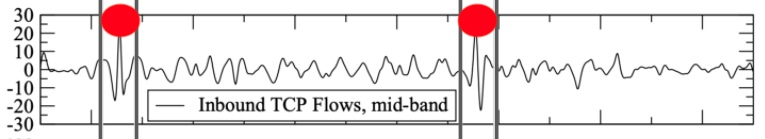
\includegraphics[width=4in]{fig/spike.jpg}
\end{center} 
All previous anomaly detection work in scientific workflow lacks (i) model optimization and (ii) a tuning study.  This is hardly ideal since much prior work    advises that using data miners without  parameter optimizer leads to sub-optimal results~\cite{agrawal18, fu2016tuning, spike_jc_19}.
PI Menzies and Mr Tu showed that for workflows seen at the Pegasus research group,   
standard anomalies learning tools for faulty TCP file transfers (without tuning) can be considered \textit{harmful} and \textit{misleading} to the reliability of networked infrastructures~\cite{tu2021mining}. 
%Among the cyberinfrastrucutre, such anomalies may change the experimental results that lead to scientific progress can be forestalled and discovery results can be even refuted.
Their proposed improvement utilized better data mining methods; specifically,
 an ensemble model (XGBoost~\cite{xgboost}) and a sequential model-based tuner (FLASH~\cite{flash_vivek}). They found that
\bi 
\item Tuning  learners will improve the relative performance up to 28\%, 29\%, and 40\% for F-measure, G-score, and recall   from the prior state-of-the-art  work~\cite{tcp_indis_19}. 
\item Tuning changes previous conclusions on what learner is the best performing, i.e., from random
forests (as recommended by prior work) to XGBoost (recommended by this work).

\item Tuning changes previous conclusions on what  factors are most
influential in detecting for anomalies by 30\%. That is, a side-effect of this work
is that it is time to change what we monitor for. 
\ei
  \\\hline
 \end{tabular}
  \end{table}
Computational considerations suggest that, of the above five tactics, we will be able to apply Tactics1,2,3 more often than Tactics4,5.
Tactics1,2,3 are data mining methods that can easily scale-up
to many   projects. Tactic4 is slower since, for each project,
it must re-run the learners hundreds to millions
of times (to learn the best tunings for that project). Lastly, Tactic5 might be slowest of all since it could
require  pre-training a neural net of  a very large corpus of CSS code.

 \label{tactics2}
\textcolor{red}{{\bf Measurable Outcomes:}} For   tactics 1,2,3 we can assess the results of our interventions using the  
    {\bf a,b,c what-if procedure} defined   at the end
of \S\ref{mm}
(on page \pageref{abc}). Also, for tactic3's self-admitted technical debt, 
if we   track the levels of technical debt in a project (using our data miners) 
and the metrics
of \fig{health}, then
then we can detect if our
technical debt reductions are having benefits within a projects.
As to tactics4,5 the outcomes we want to measure would need to be tuned to specific systems we are tuning or 
for which we are generating recommendations. 
 
 


\subsection{Research Goal3:  achieve Goal1,Goal2 via   minimal data collection}\label{goal3}

Given the size of the CSS community, the above goals may only be widely applicable if we can tame the data
collection cost associated with this kind of analysis.  
To understand that collection cost, we note
that any data miner uses large databases of $x,y$ examples to generates a model
$f$ of the form:
\[
y=f(x)
\]
Here, $x$ is project information 
(such as lines of code, number of recent updates, number of developers, etc) and $y$ is information about project performance (such as the ease of use of this code, the penetration of this code, the cost of developing the code).
Given access to Github, it is now possible to automatically collect $x$ data fro a very large number of projects. However, collection accurate $y$ is another matter.
Even when projects offer $x,y$ data, the $y$ labels
are often questionable. 
For example,  Yu et al. checked the $y$ labels
 (about software defects)
 from one Github project and
 found that more than 98\% of
the false positives (reported by prior work) were actually true positives, casting doubt on
work that used the original dataset~\cite{jitterbug}.
PI Menzies' graduate student Mr. Huy Tu~\cite{tu2019better} has developed cost models describing the effect required to check these $y$ labels where:
\bi
\item
Data is checked by pairs  of web-based crowd-sourced  workers using the Amazon Mechanical Turk facility (so results are not accepted unless two people
 agree on the label).
\item
The crowdworkers are assessed by questions with known answers (so we can prune unreliable  workers).
\ei
According to the Tu model,   it would take 
200,000 hours and cost \$2,100,000 to  review the $y$ values related
to known defects in the $\approx 700$ CSS projects we can find in Github. 

To say the least, such large costs
are   unacceptable.
Hence, Mr. Tu went on    to investigate
{\em semi-supervised methods} for reducing the cost associated with labelling Github data.
Working with non-CSS data, Mr Tu found that he could build effective software quality prediction models
by labelling just 2.5\% of the data~\cite{tu21Frugal}. Note that a 2.5\% reduction   reduces that \$2,100,000 to \$52,500 which, is spread out of a three year NSF projects becomes more acceptable at \$17,500 per year (a much more reasonable sum). 

For a brief tutorial on semi-supervised learning, see Table~\ref{inside}.
Note that none of those methods have yet to be  tested on CSS software. Nor have they been used
when trying to achieve {\bf Goal1,Goal2}. Hence...


\textcolor{red}{{\bf Measurable Outcomes:}} To test the effectiveness of semi-supervised 
learning for reasoning about CSS projects, we would generate ``trade-off graphs''
where we repeat the analysis of {\bf Goal1, Goal2} using fewer and fewer
$y$ levels (selected by  semi-supervised learning). {\bf Goal3} would be declared achievable
if we can achieve competency for {\bf Goal1, Goal2} after labelling 2.5\% (or less) of the
data.
\begin{table}[!t]
  \caption{A brief tutorial on semi-supervised learners 
}\label{inside}
 \small
 \begin{tabular}{|p{6.35in}|}\hline
 
 {\em Semi-supervised learners}~\cite{mit06}  train their models by
combining a small amount of labeled data ($Y$ values) with a large amount of unlabeled data ($X$ values).
More specifically, 
  semi-supervised algorithms~\cite{mit06}  
utilize
{\em manifold}, {\em continuity},
and {\em clustering}
assumptions.
The {\em manifold} assumption is that data
lies approximately on a manifold of a much  lower dimension than the input space.
Under this manifold assumption, higher-dimensional data
is approximated in a much lower dimension space, with little or no performance loss~\cite{NIPS2004_74934548}. 
When  data is spread over just a few underlying dimensions, then there are fewer ways that examples can differ.
Hence, there is more 
{\em continuity} between 
nearby examples and we do not need to reason separately about each example. Rather,
we can {\em cluster} similar examples and  reason about one item per cluster. 
Using those assumptions, there are many ways to extrapolate from a small number of labels to a larger set of data~\cite{zhu2005semi}.
For example, here we see a   recursive bi-clusters
the data down to $n=\sqrt{N}$ of the data: 

\begin{center}
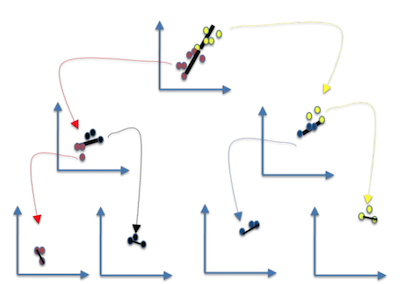
\includegraphics[height=3.6cm]{fig/fastmap.png}\hspace{1cm}
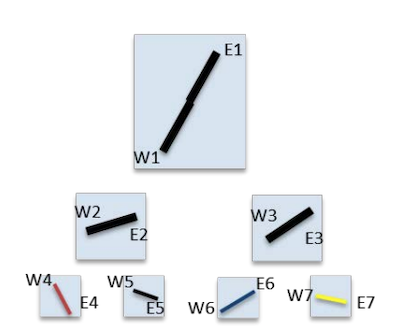
\includegraphics[height=3.6cm]{fig/tree1.png}
\end{center}

This tree of clusters was
generated via a recursive
  FASTMAP procedure~\cite{faloutsos1995fastmap}. Here, 
  $M$ is any example (selected at random).
  $E$  (east) is an example   furthest from $M$ and 
  $W$ (west) is an example   furthest from $E$.
  Note that $E,W$ can be found in time
  $O(2N)$.
  If  
  $c=dist(E,W)$ then
    other examples have distances $a,b$  to $E,W$, respectively and distance
    \mbox{ $x=(a^2+c^2-b^2) / (2c)$}
    on a line from  $E$ to $W$.
  By
splitting   data on   median $x$,
the examples can be then bi-clustered.
After generating the leaf clusters,
we can  (i)~evaluate just the centroid of each cluster;
then (ii)~propagating that label to all other items in that leaf.

As to other SSL approaches,
 {\em self training} algorithms~\cite{Yarowsky}  incrementally
guesses new labels from a learner
trained on all labels  seen to date.
Further, {\em GMM with expectation-maximization} algorithms~\cite{jonathonGMM}
use a Gaussian mixture
model to cluster the data (and use those clusters to label the data).
Furthermore,
 {\em label propagation algorithms}~\cite{Zhu02learningfrom} guess
labels using a majority vote across the labels  seen in nearby examples (or clusters).
Label propagation algorithms never update their old labels.
 {\em Label spreading} algorithms~\cite{Zhou04}, on the other hand,
update old labels using with feedback from subsequent labelling.
Label  spreading algorithm iterates on a similarity matrix
between example and   normalizes the edge weights by computing the normalized graph
of the Laplacian.\\\hline
\end{tabular}
\end{table} 


\subsection{Research Goal4:  get our recommendations used by CSS community}\label{goal4}

All the above work is pointless unless we can convince the
CSS community to use our results. In this regard, 
our experience offers much hope that these results
will be widely adopted. What we found is that if we go to projects with lists of problems and proposed improvements from that project,
then we find a ready audience. For example:
\bi
\item See the work documented in Table~\ref{casestudy};
\item We spend 2021 in bi-weekly meetings with the Linux kernel
team, discussing how our data mining results can improve their code.
\ei
In our experience, the only thing stopping the widespread
adoption of our prior results was the COVID crisis (that forced
many teams into working less with other teams and more with their
own internal workers). For the period 2022-2025 we anticipate far fewer problems with
COVID and much more collaboration between CSSI teams.


In any case, it will be important to track the application of these results. Hence:

\textcolor{red}{{\bf Measurable Outcomes:}} We will   log all our interactions with CSSI projects. We foresee that these interactions
will take three forms: (a)~initial tentative contacts;
(b)~preliminary results; (c)~review of impact, 12 months later.
We would say that {\bf Goal4} is achieved if our contacts is effective and frequent:
\bi
\item By ``frequent'', we are aiming for a least one tentative contact per month and four sets of preliminary results per year.
\item By ``effective'', we would use the same measurable outcomes
as seen in {\bf Goal3}.
\ei


\subsection{Research Goal5:  apply our methods to  CSS projects not stored in Github}\label{goal5}

For most of this project, we have assumed using data
from Github. But not all projects are stored in the location.
hence we need to check of our methods work for data from other venues.

We view {\bf Goal5} as being 
strongly connected to {\bf Goal4}. As a side-effect of all
the interactions associated with that goal, we will find
examples of code that is stored in locations other than Github.

What happens after that depends on the nature of those other sources:
\bi
\item
If these other locations support large scale data access
via web-based methods, we anticipate that our tools will readily transfer to other venues.
\item
Otherwise, we may be unable to achieve this goal.
\ei
In any case, it is important to track this issue:


\textcolor{red}{{\bf Measurable Outcomes:}} We will log all the non-Github sources found as part of this work. Also,
we will   log when (or if) our tools can achieve {\bf Goals1,2,3,4}.


\subsection{Research Goal6:  demonstrate that there exists a set of general methods   for improving CSS projects}\label{goal6}


Ideally, science can produce general
conclusions that hold in multiple contexts.
By that measure, how much of the above 
is ``scientifiic''? 

To say that another way,
what is the external validity of the conclusions reached
via the above methods? If we studied (say) 700 CSS projects, would we find general principles that hold across all these projects?
Or are all CSS projects are fundamentally different and nothing
can be generalized from one project to another?

 Before answering these quetions, we first motivate {\em why} they are worthy of discussion.
 If we could find a small number of models that represent the rest then that would have several benefits:
\bi
\item {\bf Training newcomers:} new CSS developers could be initiated by getting them to study the factors leading to CSS  project success or failure.
\item {\bf Tool development:} new tool development for CSS software could be focused
on the issues that our models find are most prevalent and most important for mitigating unhealthy project.
\item 
{\bf Early code quality improvement:} Suppose the year is 2026 and   this proposal found how CSS projects divide into communities. Suppose further
that the methods of this proposal have found quality predictors and effective plans for each of those communities. Now, new CSS
projects could quickly find the predictors and improvement plans most relevant to them {\em without running any of the tools of this project}just by (a)~finding its community; then (b)~looking up the predictors and plan known to work in that community.  
\ei
But what is the pragmatic reality about the probability of   general principles for 
improving CSS software?
Given the diversity of CSS systems, it seems unrealistic to believe that some single model holds for all projects. 
But if we cannot learn single models (for predicting project success) across all CSS projects, then perhaps we can find communities of projects with similar properties. If so, then to
reason about some new project, we need only know what ``community''the new project belongs to (after which, we can apply lessons learned from current members of that community).

Technically speaking, {\bf Goal6} is a 
{\em transfer learning task}~\cite{KrishnaMF16,Nam13,Ma2012,jing15,Kocaguneli2014,yu2017feature,jamshidi2017transfer,pan2009survey,qing2015cross,li2018cost};
i.e. what lessons about one kind of project can be transferred
to another.  To the best of our knowledge,
the transfer of knowledge (about predictors and plans for project success or failure) has not been previous explored for CSS code.
There are many reasons for using transfer learning.  Transfer learning can be useful when there is insufficient local data. Clark and Madachy~\cite{clark15} in their study of 65 software under-development by the US Defense Department in 2015 showed developers working in an uncommon area often benefit from transferring knowledge from more common areas.

One way to characterize transfer learning
methods
is the approach that it follows.  Firstly, {\em dimensional transformation} methods   manipulate the raw source data until it matches the target. An initial attempt on performing transfer learning with Dimensionality transform was undertaken by Ma et al.~\cite{Ma2012} with an algorithm called transfer naive Bayes (TNB). Since then there are many such algorithms have been proposed such as TCA~\cite{Nam13}, TCA+~\cite{Nam2015}, TPTL~\cite{liu2019two}, and balanced distribution~\cite{xu2019cross} (just to name a few).


Secondly, there is another group of algorithms invented by   PI Menzies
and his student Rahul
Krishna. According to the Oxford English Dictionary, the bellwether is the leading sheep of a flock, with a bell on its neck, that all other sheep follow.
A {\em bellwether} method~\cite{krishna2017simpler,krishna16}.
assumes that within a community of software projects, there is one exemplary project called the {\em bellwether}, which can define predictors for the others. This effect is called {\em the bellwether effect}. They exploit this Bellwether effect in their {\em  bellwether method}  that searches for such an exemplar bellwether project to construct a transfer learner with it. This proposal
will use the bellwether method since our experiments shows
that it out-performs dimensionality transform methods~\cite{krishna2017simpler}.

One problem with Krishna's bellwether methods is that the algorithm requires  an $O(N^2)$ comparison of all projects-- which becomes impractical when reasoning about (e.g.) 700 CSS projects~\cite{majumder2019learning}.  To solve that problem, 
PI Menzies and his student Suvodeep Majumder have added a clustering pre-processor to the bellwether method. In this approach, data from multiple projects is recursively grouped together into a
tree of clusters and sub-clusters and sub-sub-clusters etc.
The Bellwether method is applied to each leaf and the best model
is promoted up one level. Then at each level $i$ of the cluster tree,
 the bellwether method is applied to applied to all the models promoted up from level $i+1$.  The best model (as found by the bellwether method) is then promoted to level $i-1$.
 Promotion stops when the level $i$ performs worse
 than the models found at level $i+1$. In studies with  1,628 non CSS projects,
 this hierarchically bellwether method returns just six models; i.e. those 1628 projects could be approximated by by six communities (with one model from each community)~\cite{majumder2019learning}.
 


\textcolor{red}{{\bf Measurable Outcomes:}} In this project, we would repeat the Menzies \& Majumder hierarchical analysis
on CSS projects. {\bf Goal6} would be called a success if it could be shown that, for many $N$ CSS projects,  the
benefits seen in {\bf Goals,1,2,3,4,5} could be achieved via a small number of $M$ models 
($M \ll N$) models.



practitioners and researchers to build more robust models against  white-box   adversarial evasion attacks using an new tool called \mbox{OMNI-2}.
 Many  malware and intrusion detection systems use machine learning-based   detection models. Prior work has shown that such models are susceptible to adversarial evasion attacks~\cite{dalvi2004adversarial,lowd2005adversarial,lowd2005good} where inputs are    crafted by intelligent malicious adversaries~\cite{biggio2013evasion} in order make the defender
(e.g. a neural net) misclassify malicious inputs as ``benign''. %Once the attackers can fool a classifier to think that a malicious input is actually benign, they can render a machine learning-based malware or intrusion detection system ineffective.
% We propose defeating
% adversarial learners via 
% {\bf {\em multi-objective configuration}}\footnote{All
% terms shown in {\bf {\em bold}} are explained, later in this proposal.}. 
To recognize an adversarial attack,
 a defender must configure a  
learner.  
Using   {\bf {\em multi-objective geometry tricks}} including {\bf {\em epsilon domination}}, OMNI-2 can  explore the configuration of a large number of possible    defenders, then cache
100s of {\bf {\em nearly-optimal}}, but {\bf {\em unexpectedly different}}
ones.
By jumping randomly between all those configurations, it is possible to   prevent an adversary from finding
patterns in the defenses.
Results from our OMNI-1 prototype~\cite{shu2020omni} have demonstrated the value of this approach. 
As seen in Figure~\ref{fig:contagio_distance} of page~\pageref{fig:contagio_distance} of this proposal,
the {\em greater} the 
{\bf {\em  unexpectedness}} of the defender,
the {\em better} the post-attack accuracy of OMNI-1's defense. 

The  success of   OMNI-1   suggests that  \underline{\bf prior work     made  premature and 
 incorrect conclusions}  about the value of diversity-based defences (against adversarial learning). 
  Prior work   suggested
    that    different  defending
  learners generate the  same decision boundary
  (the region separating malicious from benign inputs)~\cite{zhang2020decision,zhang2018gradient,he2017adversarial,DBLP:conf/iclr/TramerKPGBM18,DBLP:journals/corr/PapernotMG16}. This is highly
  undesirable since it  mean
   attackers can also learn that structure, {\em even if the attacker does not know
  the learner being used by the defender}.  Yet if this were always so, then OMNI-1 
  would not have worked.  The possibility, to be explored here with OMNI-2, is that  if we jump around a very large range of defense options, we can effectively defend against a wide range of adversarial attacks. 
% This work revisits the value of

To explore the value of this kind of defence with OMNI-2, we need to achieve several
goals. Firstly, we need to address certain limitations in the prior
  \mbox{OMNI-1}   study. For example,  there still remains a large gap in the pre-attack performance and then best results obtains via \mbox{OMNI-1}. Hence,   OMNI-2 must:
\begin{formal}\noindent
{\bf GOAL1:} Improve the post-attack performance. 
\end{formal}
\noindent
(For this goal, we will explore more learners and pre-processors than used in \mbox{OMNI-1}.)

Also,
\mbox{OMNI-1} took   hours to generate its population.
This is highly undesirable since this kind of   defence is most  useful when it can generate more
candidate defences. Hence, for OMNI-2, we must:
\begin{formal}\noindent
{\bf GOAL2:} OMNI-2 needs to  orders of magnitude
faster than OMNI-1. 
\end{formal}
\noindent
(This goal will be explored via the innovations of \S\ref{faster}:   
 {\bf {\em old-but-gold}}, and
{\bf {\em dumb-but-faster}}, and others.)

Further, \mbox{OMNI-1}  was tested with static adversaries that do     not adapt  
tactics while attacking. Hence:
\begin{formal}\noindent
{\bf GOAL3:} Show that \mbox{OMNI-2}  defeats  
state-of-the-art \underline{adaptive} adversaries. 
\end{formal}
\noindent
(Our pre-experimental intuition is that defending against adaptive adversarial attacks will
become another speed problem; i.e. the faster we can generate different defenses adaptively, the better we will be able to counter against attack adaption.)

 \mbox{OMNI-1}  was  
tested   on   Table~\ref{data}'s   data
and  it should be tested on   more case studies. Hence: 
\noindent
\begin{formal}
{\bf GOAL4:} Show that \mbox{OMNI-2}  works in numerous  domains. 
\end{formal}
\newpage
\noindent
With all that done, we can turn to the main point of this resaerch: 
  \noindent
\begin{formal}
{\bf GOAL5:}    Ensure that    \mbox{OMNI-2}'s defensive learners do not converge
  to the same decision boundary.
  \end{formal}
  \noindent
This goal is important shice
Khasawneh et al.\cite{khasawneh2017rhmd} and Demontis et al.~\cite{demontis2019adversarial}  argue that,
in terms of explaining how adversarial learning can defeat
an attacker,   
  the  properties of the learner  are  less important  than 
  the {\em properties of the decision boundary}.
  In our whitebox scenario, the attackers and defenders have access to the same examples.
  If an attacker can learn the same decision boundary
  as the defender, then they can always craft inputs that  confuse the defender.
 
 
  
  
  
  
  
\begin{table}[!t]

\small
\begin{tabular}{p{.98\linewidth}} 
\rowcolor[HTML]{ECF4FF}
{\bf NSL-KDD}~\cite{nsl-kdd} : an improved version of KDD'99~\cite{tavallaee2009detailed}. Records network traffic under different types of attacks. \\ 
{\bf CIC-IDS-2017}~\cite{sharafaldin2018toward}. Normal traffic and simulated abnormal data caused by intentional attacks on a test network.
\\ 
\rowcolor[HTML]{ECF4FF}
{\bf CSE-CIC-IDS2018}~\cite{sharafaldin2018toward} is  an intrusion detection dataset that  includes seven different attack scenarios (Brute-force, Heartbleed, Botnet, DoS, DDoS, Web attacks, and infiltration of the network from inside). \\ 
{\bf CICAndMal2017}~\cite{lashkari2018toward} is an Android malware dataset that collects 426 malicious and 1,700 benign applications collected from 2015 to 2017.   Malicious samples in 4 categories: Adware, Ransomware, Scareware, SMS Malware.   \\ 
\rowcolor[HTML]{ECF4FF}
{\bf Contagio PDF Malware}~\cite{contagio-pdf} dataset has  labels
on a set of benign and malicious PDF documents
(i.e. those used as delivery vechiles for
malicious content), including a relatively large number from targeted attacks.\\ 
 \end{tabular}
 \caption{Data sets used to test \mbox{OMNI-1}.}\label{data}
 \end{table}
 
 
 Yet if this were always so, then OMNI-1 
  would not have worked.   Perhaps if we explore a much larger range of defense options
  (as proposed for OMNI-2), we can find good defences against a wide range of adversarial attacks. 
  The success of \mbox{OMNI-1} is a preliminary result suggesting {\bf GOAL5} might be  achievable
  (since
 one way to explain the  observed success of \mbox{OMNI-1} is that this defender found
  different decision boundaries, thus thwarting the attackers). 
But  as stated above,   \mbox{OMNI-1} was a somewhat limited study.
  Accordingly, in this proposal, we must explore this issue more broadly.

\section{
Relevance to Secure and Trustworthy Cyberspace (material required by  solicitation)} 
\subsection{Clear and concise description of the threat model(s)}
\bi
\item
This work assumes that an {\em adversary's goal} is to impact target model’s prediction performance by causing its misclassification in the testing phase, thus 
allowing a malicious payload not being detected.
\item
Also, as to the {\em adversary's knowledge},
we assume a whitebox agent that has access to      knowledge of the defender model as well
as the examples used to train the defender. 
\item
As to the 
{\em adversary’s capability},  we assume adversarial attacks are carried out at the inference time (i.e., testing time), which means the attackers are only able to perturb the immediate inputs, while not be able to manipulate the training dataset. 
\ei
\subsection{Discuss the generalizable theories and research methods that will be developed.} {\bf GOAL5} is
a very general point that speaks to core nature of machine learning.

As to generality of what OMNI-2 can recommend for different data sets, this work will be tested
on a wide range of data sets (including Table~\ref{tbl:securityDataset}, and  other data we   find 
during the course of this research).


Another generalizable result is what this says about  
 ensembles, and their value for  defending against attackers. Ensemble defences has is proponents~\cite{kariyappa2019improving,biggio2010multiple,DBLP:conf/iclr/TramerKPGBM18,smutz2016tree,kantchelian2016evasion} and it detractors~\cite{zhang2020decision,zhang2018gradient,he2017adversarial,DBLP:conf/iclr/TramerKPGBM18,DBLP:journals/corr/PapernotMG16}. 
 We argue here before we can use ensembles to defend against attackers, we need to change the way we build and use ensembles.  
Instead of averaging out multiple conclusions, OMNI  uses conclusions
from a large number of learners {\em all of which are  very
different from each other}\footnote{For an operational definition of ``very different'', see page \pageref{definititions}
of this proposal.}.
That is to say, 
 OMNI's conclusions come from exploring the 
 {\em far corners of a very large ensemble}, rather than just the center
of a   small ensemble. 

\subsection{Discuss the trade-offs and risks involved in the research plan}
See our research plan, below, in
\S\ref{r1}, \S\ref{r2}, \S\ref{r3}, \S\ref{r4} and \S\ref{r5}.
 
 
 
 
 
 \section{Motivation and Related Work}\label{back}
 
 The global security threat continues to evolve at a rapid pace, with a rising number of types of threats.
 In the social network realm, Facebook estimated that hackers stole user information from nearly 30 million people through malicious software~\cite{facebookreport}.
According to the International Data Corporation (IDC), the Android operating system covers around 85\% of the world’s smartphone market. Because of its increasing popularity, Android is drawing the attention of malware developers and cyber-attackers. Android malware families that are popular are spyware, bots, Adware, Potentially Unwanted Applications (PUA), Trojans, and Trojan spyware, which affect millions of Android users~\cite{bhat2019survey}.
 With the growing reliance on information technology, cybercrime is a serious threat to the economy, military and other industrial sectors~\cite{bissell2019cost,jang2014survey,chang2019evaluating,opderbeck2015cybersecurity,rovskot2020cybercrime}. 
In 2019, the damage cost caused by malware and cybercrime exceeded a trillion dollars~\cite{morgan2019official}. For example, a March 2019 ransomware attack on aluminum producer Norsk Hydro caused 60 million pounds of remediation cost~\cite{sechel2019comparative}. The attack brought production to a halt at 170 sites around the world. More generally, a 2019 study by Accenture reports that cybercrime will cost US \$5.2 trillion over the next five years~\cite{bissell2019cost} Alarming, that cost is growing.  That same report documents that in the United States, the annual average cost to organization of malicious software has grown 29\% in the last year. 


There are many kinds of malicious software.
{\em Malware}   is a malicious file or hidden within files; e.g. PDF files can carry malicious code~\cite{smith01}.
{\em Ransomware}  encrypts a victim's files then demands a ransom from the victims to restore access to the data upon payment. For example, a March 2019 ransomware attack on aluminum producer Norsk Hydro caused 60 million pounds of remediation cost. The attack brought production to a halt at 170 sites around the world (some 22,000 computers were affected across 40 different networks)~\cite{sechel2019comparative}. 
{\em Industrial espionage software} infects, then destroyed industrial machinery; e.g. the Stuxnet virus used to damage centrifuges at Iran’s Natanz uranium enrichment facility~\cite{langner2011stuxnet}.
Other kinds of malicious software~\cite{monshizadeh2014security} include (a) {\em scareware} that socially engineers anxiety, or the perception of a threat, to manipulate users into e.g. buying unwanted software; (b) {\em adware} that throws advertisements up on your screen (most often within a web browser); and (c)~software that infects your computer then, without your permission of knowledge,   {\em mounts a denial of service attack} on other computers. 

In response to the above,
security practitioners now routinely add security detectors to their environments, which are machine learning models that utilize known detective patterns to verify whether an application becomes a threat. Such detectors can be built in many ways including (but not restricted to) building a classifier to examine a web page for malicious content~\cite{canali2011prophiler,eshete2012binspect}; constructing multiple classifier systems to classify spam emails~\cite{biggio2010multiple}; building classifiers to detect malicious PDF files~\cite{xu2016automatically};
applying machine learning to detect Android malware~\cite{grosse2017adversarial}; designing supervised learning algorithm to classify HTTP logs~\cite{liu2017robust}; designing machine learning models to detect ransomware~\cite{munoz2017towards}; and detecting malicious PowerShell commands using deep neural networks~\cite{hendler2018detecting}.


 Paradoxically, machine learning also introduces a new attack vector for motivated adversaries\cite{barreno2006can,DBLP:journals/pr/BiggioR18}.   \textit{Adversarial machine learning}  is a technique that attempts to fool or misguide a machine learning-based model with malicious inputs
 (for a sample of these methods, see  Table~\ref{attacks})
This technique was
first studied in spam filtering~\cite{dalvi2004adversarial,lowd2005adversarial,lowd2005good} and later on since 2014, Szegedy et al.~\cite{szegedy2013intriguing} found that small perturbations in images can cause misclassification in neural
network classifiers. This technique is also widely studied in the security domain. \textit{Adversarial evasion attack}~\cite{biggio2013evasion} is one of the most prevalent types of adversarial machine learning attacks that happens during the testing stage in the machine learning pipeline. In this attack, attackers try to evade the detection system by manipulating the testing data, resulting in a wrong model classification. The core of adversarial evasion attack is that when an attacker can fool a classifier to think that a malicious input (e.g., malicious Android application or network traffic) is actually benign, they can render a machine learning-based malware detector or intrusion detector ineffective.


\begin{table}[!t]

\begin{tabular}{p{.98\linewidth}} 
\small
\rowcolor[HTML]{ECF4FF}
\textit{\textbf{Fast Gradient Sign Method (FGSM)}}~\cite{DBLP:journals/corr/GoodfellowSS14} is a method to that learns the region of making loss (classifier error) by studying the gradient changes 
found in a model after   from minor perturbations to the data.
\\
\textit{\textbf{Basic Iterative Method (BIM)}}~\cite{KurakinGB17a}   iteratives over  FGSM, adding a small perturbation at  each iteration.   BIM-A       iterating once a   mislcassification is achieved.   BIM-B   
stops after a fixed number of rounds.
\\
\rowcolor[HTML]{ECF4FF}
\textit{\textbf{Jacobian-based Saliency Map (JSMA)}}~\cite{papernot2016limitations}  uses feature selection with the aim of minimizing the number of features perturbed (i.e., the $L_{0}$ distance metric) before a misclassification is achieved.
\\
\textit{\textbf{DeepFool}}~\cite{moosavi2016deepfool} works iterative to  minimizing the   distance between perturbed   and original data (i.e., the $L_{2}$ distance metric).   Adversarial 
examples are generated
via a linear approximation of the decision boundary that  different classes, and then adding a perturbation perpendicular to that decision boundary, which brings the input closest to a linear approximation of the decision boundary.  
\\
\rowcolor[HTML]{ECF4FF}
\textit{\textbf{Carlini-Wagner (C \& W)}} attack~\cite{carlini2017towards,DBLP:conf/ccs/Carlini017} is an optimization tactic that seeks the smallest noise  added to input $x$ that   changes the classification to a class $t$ (in our case, from malicious to benign).
\end{tabular}
\caption{Examples of adversial attack methods.}\label{attacks}
\end{table}


Prior studies have tried~\cite{DBLP:conf/iclr/TramerKPGBM18,smutz2016tree,kantchelian2016evasion} to thwart evasion attacks by building a more robust and complex model via \textit{ensemble learning}~\cite{dietterich2002ensemble}. Ensemble learning is the process of (a)~building multiple models and then (b)~polling across the models to arrive at a final decision. 
For example, Biggio et. al.~\cite{biggio2010multiple} investigated ways to build a multiple classifier system (MCS) that improved the robustness of linear classifiers. Tramer et. al.~\cite{DBLP:conf/iclr/TramerKPGBM18} introduced a technique called ensemble adversarial training that augments training data with perturbations transferred from other models to increase robustness. Kariyappa et. al.~\cite{kariyappa2019improving} showed that an ensemble of models with misaligned loss gradients is an  effectively defence mechanism.


In theory, ensemble learning defend against adversarial evasion attack since attackers have to craft payloads (i.e., adversarial examples) that are able to subvert all constituent models at once.
However, some  studies~\cite{zhang2020decision,zhang2018gradient,he2017adversarial,DBLP:conf/iclr/TramerKPGBM18,DBLP:journals/corr/PapernotMG16} caution that adversaries can still defeat ensemble-based strategy. For example, Papernot et al.~\cite{DBLP:journals/corr/PapernotMG16} find that, even when ensemble classifiers are used, adversarial attackers can still manage to use their own models to find ways to ``transfer'' the adversarial examples to a victim model (i.e., attacker's target model), even if (a)~the adversary has little knowledge of the victim model; and even if (b)~the defender uses an ensemble of classifiers.

Why do ensembles fail to defend against attackers? Once issue is that  when ensemble learning combines conclusions from ensemble methods, that ``voting'' process trends to conclusions that approximate
  the median decision boundary between classifiers. Hence, some researchers
report that  ensemble learning may not be an adequate defense against attackers~\cite{zhang2020decision,zhang2018gradient,he2017adversarial,DBLP:conf/iclr/TramerKPGBM18,DBLP:journals/corr/PapernotMG16}. For example, Zhang et al.~\cite{zhang2020decision} show that a discrete-valued tree ensemble classifier can be easily evaded by adversarial inputs manipulated based only on the model decision outputs.  Papernot et al.~\cite{DBLP:journals/corr/PapernotMG16} find the transferability property of adversarial examples  (where two different learners working on the same data generate the same decision boundary) also make ensemble classifier less effective. 


Can we build ensembles in a different manner, making them better suited to adversarial defence? Perhaps so, and we some evidence that supports
that conjecture.
(see the results from the OMNI-1 research  in
 Figure~\ref{fig:contagio_distance} of page~\pageref{fig:contagio_distance} of this proposal).
 We began working on   OMNI after observing that
{\em 
prior work on ensemble learning against adversarial evasion attack barely explored the vast range of configurations available within a model or explored few different models. }
As shown in Table~\ref{tbl:hyperparameters}, 
malware or intrusion detection models can be built from a space of trillions of configurations (i.e., hyperparameter choices of a model). 
Yet   researchers build their ensemble-based approaches using a small number of constitute models; e.g., Kantchelian et al.~\cite{kantchelian2016evasion} use seven constitute models in their ensemble classifier. Strauss et al.~\cite{strauss2017ensemble} use an ensemble of ten classifier as the defense strategy against adversarial perturbations.
Hence it is possible that we can  
\underline{\bf defeat adversaries by building defences  
    from a   very large set of possible  configurations.}
 

Another concern we had with prior work was
that   
the smoothing out of individual variations
(via ensemble voting) can make a decision boundary smoother, and hence easier to predict (and attack). 
An alternate approach, used by OMNI is to   {\bf not}
to average across a collection of learners but, instead
\underline{\bf defeat adversaries  by selecting  defenders from the corners of a   very large set of possible  configurations}. 




 \section{About OMNI}\label{back}
% PI Menzies has had some   success with automatically explore
% large sets of configurations for
%   software
% problems. His 2002 paper with Martin Feather (from JPL) is one of the earliest applications
% of concepts of multi-parameter optimization to software requirements engineering~\cite{DBLP:conf/re/FeatherM02}. In more recent work, he 
% has
% explored stochastic optimizations methods for configuring video encoding software~\cite{chen2018sampling},
% aircraft control software~\cite{DBLP:journals/tse/KrallMD15},
% and cloud computing control methods~\cite{chen2017riot} in $O(n.log(n))$ time. Whereas
% other method might take hours to days, many of PI Menzies' stochastic
% algorithms terminate in seconds
% to minutes (depending on the model).


\begin{table}[!t]
\centering

\footnotesize
\begin{threeparttable}
\begin{tabular}{|r@{~:~}l|} 
\hline
\rowcolor[HTML]{ECF4FF} \textbf{Hyperparameter} & \multicolumn{1}{l|}{\cellcolor[HTML]{ECF4FF}\textbf{Ranges}} \\ \ 
\begin{tabular}[c]{@{}c@{}}Hidden layer  activation function\end{tabular} & \begin{tabular}[c]{@{}l@{}}elu, relu, selu, sigmoid, softmax, tanh, hard\_sigmoid, softplus,    softsign,  linear, exponential\end{tabular} \\  
\begin{tabular}[c]{@{}c@{}}Output layer  activation function\end{tabular} & \begin{tabular}[c]{@{}l@{}}elu, relu, selu, sigmoid, softmax, tanh, hard\_sigmoid, softplus, softsign,  linear, exponential\end{tabular} \\  
First layer dense & quniform(30, 150, 1) \\  
Second layer dense & quniform(30, 50, 1) \\  
Third layer dense & quniform(10, 32, 1) \\  
Drop out rate & uniform(0.0, 0.5) \\  
Optimizer & \begin{tabular}[c]{@{}l@{}}Adadelta, Adagrad, Adam, Adamax,   NAdam, RMSprop, SGD\end{tabular} \\  
Batch size & 16, 32, 64, 128 \\ 
Number of epochs & quniform(5, 20, 1) \\  
Learning rate & 0.001, 0.01, 0.1 \\ \hline
\end{tabular}
\begin{tablenotes}
    %   \small
\item  \textbf{quniform($low$, $high$, $q$)} means $round(uniform(low, high)/q) * q$. \textbf{uniform($low$, $high$)} returns a value uniformly from $low$ to $high$.
% \item * Note-2: We do not optimize the number of hidden layers but use 3 layers in our study, since we observe that they are enough for us to make good predictions and speed up the training process.
\end{tablenotes}
\end{threeparttable}
\caption{Prior explorations of
the hyperparameters of adversarial defenders  explored just dozens to hundreds of possibilities. This barely scratches the  surface of the large space of possible hyper-parameter options. For example,
here are the hyperparameters for a   deep neural networks Assuming the drop out rate is divided into 100 options, then this table shows around $10^{13}$ options: 
$11*11*120*20*22*100*7*4*15*3$.}
\label{tbl:hyperparameters}
\end{table}

 
% The core innovation of OMNI is to:
% \bi
% \item Use   {\em hyperparameter optimization}~\cite{feurer2019hyperparameter} to generate  a   very large ensemble of possible  configurations.
% \item Prune that ensemble by selecting 
% {\bf {\em near optimal}}, but {\bf {\em unexpectedly different}} configurations.
% \ei
The last section suggested that we can build better adversarial defences by working across   very large set of very different learners.
One  way to generate a very large space of different learners is via  
  automatic hyperparameter configuration.
{\em Hyperparameter optimizers} are algorithms that   seek the control
settings of a  machine learning algorithm that most improves its performance.  In a machine learning algorithm, hyperparameters are properties that control the behaviors of the machine learning algorithms. For example, when reasoning about ``$k$-nearest neighbors'', the hyperparameter ``$k$'' decides how many neighbors to use for making a decision. And when reasoning about
configuration parameters for a learner designed
to detect adversarial input, the hyperparameters
might be the control parameters of
a deep learner  seen in
Table~\ref{tbl:hyperparameters}.

 

\begin{wraptable}{r}{2.5in}
\centering
\footnotesize
\begin{tabular}{|rcc|}\hline
\rowcolor[HTML]{ECF4FF} &Metrics   & Definition                                    \\  
$y_1$=&Accuray   & (TP$+$TN)$/$(TP$+$TN$+$FP$+$FN)                         \\ 
$y_2$=&Precision & TP$/$(TP$+$FP)                                    \\ 
$y_3$=&Recall    & TP$/$(TP$+$FN)                                    \\  
$y_4$=&False Alarm &TN$/$(TN$+$FN)\\
$y_i=$& etc. &\\
\hline
\end{tabular}
\caption{Objectives based on true negatives (TN), false negatives (FN), true positives (TP) and false positives (FP).}\label{tab:metrics2}
\end{wraptable}

There are many hyperparameter optimization
techniques such as (a)~genetic algorithms
that mutate a population across many generations
to find good solutions~\cite{goldberg1988genetic};
(b)~differential evolution~\cite{price2006differential};
(c)~various reinforcement learning schemes~\cite{MAZYAVKINA2021105400};
(d)~Bayesian parameter optimization algorithms
such as Hyperopt~\cite{bergstra2012random}
or SMAC~\cite{Hutter11} that reflect
on small models built so far in order to select
what to test next;
(e)~PI Menzies' geometric learning schemes that
reflect over the shape of the example seen so far in order
to decide where to sample next~\cite{chen18}; and many more.

 
OMNI extends standard hyperparameter optimization with some 
{\bf {\em multi-objective geometry tricks}}. 
To understand these tricks, we first have to discuss the {\em twin spaces} of optimization shown in Figure~\ref{moo}.
When optimizing some function \[y_1,y_2,...\;=\;f(x_1,x_2,x_3,....)\]
the independent $x_i$ variables are the things we alter and the
dependent $y_i$ variables are the effects associated
with those alterations. For example, if hyperparameter settings from an adversarial
defender are the  
the $x_i$ variables then  the $y_i$ variables could be the performance
scores seen when that learner is deployed as an adversarial defender (see  Table~\ref{tab:metrics2}).

\begin{figure}[!t]
\caption{In this multi-objective optimization
problem $y=f(x)$ and the best models are those that result in (e.g.)
low false alarms and high recalls (i.e. the top-left region of the right-hand-side
objective space). Similar decisions
usually have similar   objective scores (see   purple and brown points). But sometimes, similar objective scores arise from very different decisions
(see the orange points).   }\label{moo}
\begin{center} 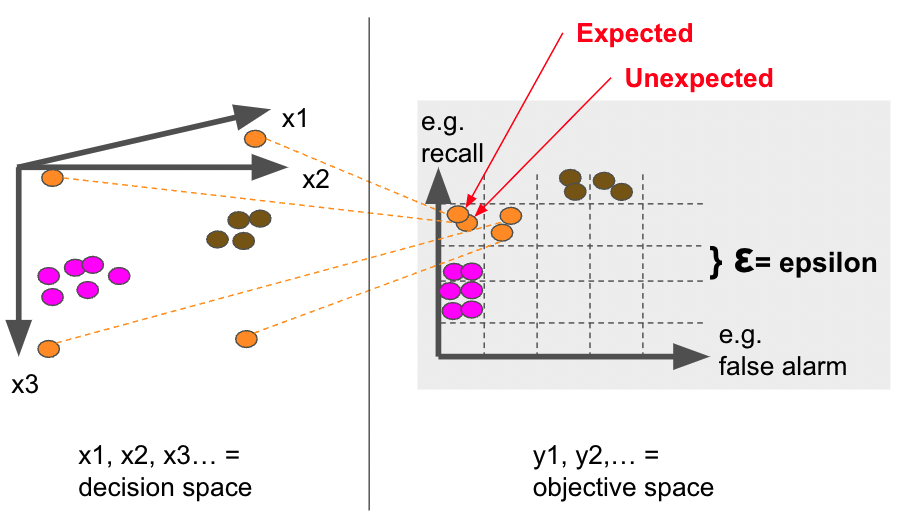
\includegraphics[width=4in]{fig/yfx.png}\end{center}
\end{figure}
In the usual case, similar $x$ decisions lead to similar $y$ results (see the brown and purple points of Figure~\ref{moo}). But sometimes,
as shown in   orange  in Figure~\ref{moo}, very different $x$ decisions 
lead to the same $y$ values.  This suggests the following tactic:
\bi
\item

In our whitebox scenarios, attackers and defenders   access   the same examples and know the range of parameters available to the defender's learners.
In this case, attackers might   explore a range of configurations 
to find the best one-- which we   marked as ``Expected" in  Figure~\ref{moo}
(this configuration is ``best'' and ``Expected" since it has lowest false alarms and
most recall).
\item

But also in Figure~\ref{moo}, we can see that very close to ``Expected'' is an 
{\bf {\em nearly-optimal}},  but {\bf {\em unexpectedly different}} configuration
which we have marked as ``Unexpected''. We say it is unexpectedly different 
since it comes from a very
different part of the decision space to the expected configuration.
\item
If the  attacker  tries to confuse the ``Expected'' configuration, but the defender
is using the ``Unexpected'' configuration then, as seen with OMNI-1, that  attack can fail.
\item
Further, if the defender learns a large cache of nearly optimal but unexpectedly
different configurations, then switches randomly between them for each new input,
then, theoretically, that could exhaust the defender's ability to design inputs that
confuse that large space of defenders. OMNI-2 will explore this possibility.
\ei
(Aside: this all    assumes   samplings of different configurations
do not converge to the same decision boundary-- hence {\bf GOAL5},
listed on page~1). 

We say that a configuration is:\label{definititions}

% \begin{table}
% \caption{Results from the \mbox{OMNI-1} prototype. From~\cite{XXX}.}
% \begin{tabular}{|p{.98\linewidth}|}



\bi
\item
{\bf {\em Nearly-optimal}} if its
$\Delta{y}$ distance to the ``Expected'' configuration is 
{\em small}
\item
{\bf {\em Unexpectedly different}}
if its $\Delta{x}$ distance to the ``Expected'' configuration is 
{\em large} 
\ei
(where $\Delta{y}$ is computed across the objective space and $\Delta{x}$
is computed across the decision space).

To operationalize {\bf {\em nearly-optimal}},  but {\bf {\em unexpectedly different}}, \mbox{OMNI}   needs a distance function that works in decision or objective space. While objective space values are all numeric, decision space variables
might be discrete (e.g. some policy setting {\em true} or {\em false} denotes enabling some feature of a learner). 
The 
\textit{Gower distance}~\cite{gower1971general} of
Equation~\ref{eqgow} is a distance measure   for such heterogeneous spaces:

\begin{center}
{\small
\begin{minipage}{.25\linewidth}
{\small \begin{equation}\label{eqgow}
    d(i,j) = \frac{\sum_{k=1}^{N} w_{ij}^{(k)}d_{ij}^{(k)}}{\sum_{k=1}^{N} w_{ij}^{(k)}}
\end{equation}}
\end{minipage}\hspace{.7cm}\begin{minipage}{.25\linewidth}
\begin{equation}\label{eqcat}
    d_{ij}^{(k)} =  
    \begin{cases}
    1, & \text{if} \: x_{i}^{(k)} \neq x_{j}^{(k)}\\
    0, & \text{if} \: x_{i}^{(k)} = x_{j}^{(k)}
    \end{cases}
\end{equation}  
\end{minipage}\hspace{.7cm}\begin{minipage}{.3\linewidth}
\begin{equation}\label{eqnum}
    d_{ij}^{(k)} = \frac{|x_{i}^{(k)} - x_{j}^{(k)}|}{max(x^{(k)}) - min(x^{(k)})}
\end{equation}\end{minipage}}
\end{center}
Here, $w_{ij}^{(k)}$ is the weight of variable $k$ between observation $i$ and $j$ and $d_{ij}^{(k)}$ is the distance between $i$ and $j$ on variable $k$. Moreover, $d_{ij}^{(k)}$ applies different formulas to categorical and numerical variables.
In Equation~\ref{eqcat},
  if two categorical observations are the same then the distance $d_{ij}^{(k)}$ of them is assigned $0$, otherwise assigned $1$.
  In Equation~\ref{eqnum},
  For numerical variable, the absolute difference is calculated between observation $i$ and $j$, then the result is scaled to range $[0,1]$ by dividing the range of values of variable $k$.  Note that, in both equations,  
 all these distances $d_{ij}$ are normalized 0..1 for min..max.


 Equation~\ref{eqgow} lets us test the core assumption of  OMNI\footnote{
 As stated on the last page, the core assumption of OMNI is effective
defenders against adversarial attacks can be built from 
configurations that {\bf maximizes} the $\Delta{x}$ distance
(to the ``Expected'' configuration)
while {\bf minimizing} the 
  $\Delta{y}$ distance.}. Figure~\ref{fig:contagio_distance} show post-attack classification accuracies (for recognizing ``malicious'' attacks)  using \mbox{OMNI-1} using an    ensemble built from  $\Delta{y}\le 0.05$ 
  and $\Delta{x}\in \{0.1, 0.3. 0.5, 0.7, 0.9\}$.
  Note that   
  across all six adversarial method studied here,
  the larger the  $\Delta{x}$, the greater the post-attack accuracy.   The improvement can be very striking.
  E.g. for BIM-A, \mbox{OMNI-1} triples the post-attack accuracy. 


\begin{figure}[!t]
\caption{\mbox{OMNI-1} post-attack classification \textit{accuracy} (\%) seen on the Contagio PDF
data set seen for 
$\Delta{x}\in \{0.1, 0.3. 0.5, 0.7, 0.9\}$ (see the x-axis). 
For details on this data set, see Table~\ref{data}.
For details on the attack methods, see Table~\ref{attacks}. 
For a definition of accuracy (on the y-axis),
see Table~\ref{tab:metrics2}.
These results are median values seen when 
the data was  as split  five times into   80\% (for   training and   optimization) and 20\% for final model testing.
The training set was    further split with ratio 3:1
where our hyperparameter optimizer trained with the former part (75\%), and then evaluated in the latter part (25\%). While this figure shows results from one data sets,
recent work~\cite{shu2020omni}  sows that the   pattern seen here (that increasing $\Delta{x}$ improves post attack accuracies) also occurs in all the data sets of Table~\ref{data}. }\label{fig:contagio_distance}
\centering
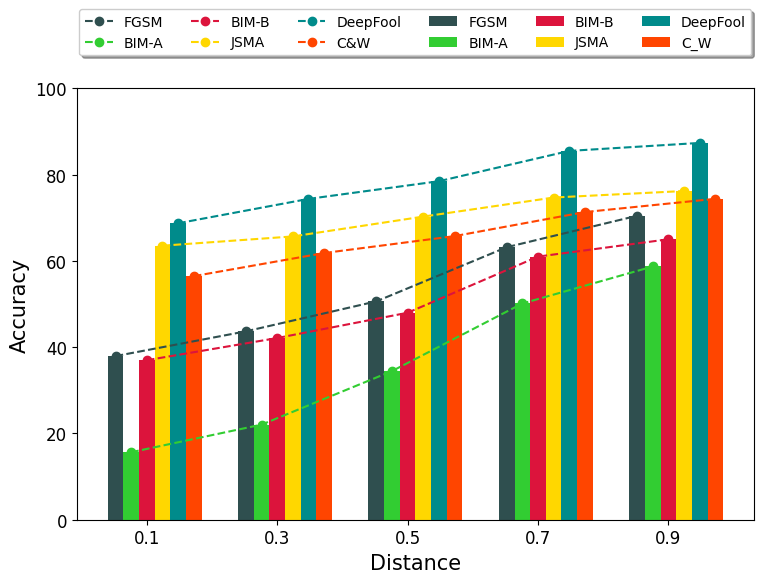
\includegraphics[width=11cm]{fig/contagio_distance.png}

\end{figure}

 


Recently~\cite{shu2020omni}, PI Menzies and his former graduate student Dr. Shu have repeated the analysis of
 Figure~\ref{fig:contagio_distance}
 across all the data sets of Table~\ref{data}
 and all the adversarial attack methods
of  Table~\ref{attacks}.
In a result endorsing the core
assumption of this proposal,
across all those data sets and across all those attack methods, the effect is the same; i.e.    increasing the diversity of the ensemble
methods (i.e. increasing
$\Delta{y}$) also increases the post-attack accuracy.  

\newpage
\noindent As seen in Table~\ref{tbl:contagioAccuracy},  Menzies and Shu have also compared OMNI-1  to other defense strategies:
\bi
\item[{\bf R1:}]  Do nothing;
\item[{\bf R2:}]  A basic ``adversarial training''
method~\cite{DBLP:conf/iclr/TramerKPGBM18,DBLP:conf/iclr/NaKM18,DBLP:conf/iclr/MadryMSTV18,DBLP:conf/iclr/FarniaZT19};
\item[{\bf R3:}] 
Building an ensemble from random members of the final population of ``good'' configurations found by 
Bergstra
Hyperopt/TPE algorithm~\cite{Bergstra:2012}, but 
with no consideration on $\Delta{x}$;
\item[{\bf R4:}] A cut down version of OMNI-1.
that neglects to weigh ensemble members
according to the known performance of
that member;
\item[{\bf R5:}]  Full OMINI-1.
\ei

 
\begin{table}[!b]
 \small

\begin{tabular}{|p{1.5cm}|p{1.5cm}|p{2cm}|p{2cm}|p{2cm}|p{2.5cm}|p{2cm}|p{2cm}}
\cline{3-7}
\multicolumn{2}{c}{~}&\multicolumn{5}{|c|}{Post-attach accuracy after using   $R1,R2,R3,R4,R5$  }\\ 
\multicolumn{2}{c}{~}&\multicolumn{5}{|c|}{to defend against the attacks shown in column one.}\\\cline{2-7}
\multicolumn{1}{p{1.4cm}|}{
~\newline
~\newline~\newline
Attack }& $R0$:\newline Pre-attack  defender accuracy& {\bf R1}: \newline Attack impact (no defense)&
{\bf R2}: \newline Basic\newline defense & 
{\bf R3}:\newline Standard \newline  ensembles & 
{\bf R4}: \newline \mbox{OMNI-1} minus \newline   ensemble weights & 
{\bf R5}: \newline \mbox{OMNI-1}\newline \\\hline
BIM-A    &\multirow{6}{*}{~~~~~~~93}& 14 & 55 & 23 & 51 & \textbf{59} \\ \cline{1-1}\cline{3-7}
BIM-B    && 36 & 61 & 37 & 53 & \textbf{65} \\ \cline{1-1}\cline{3-7}
FGSM     & & 38 & 59 & 34 & 58 & \textbf{70} \\ \cline{1-1}\cline{3-7}
C\&W     && 55 & 66 & 46 & 65 & \textbf{74} \\ \cline{1-1}\cline{3-7}
JSMA     && 63 & 73 & 57 & 70 & \textbf{76} \\ \cline{1-1}\cline{3-7}
DeepFool && 67 & 71 & 55 & 73 & \textbf{87} \\\hline
\multicolumn{7}{|p{.95\linewidth}|}{}\\
\multicolumn{7}{|p{\linewidth}|}{
This figure shows
 six treatments.}\\
\multicolumn{7}{|p{\linewidth}|}{\rowcolor[HTML]{ECF4FF}
 {\bf   $R0$}: {\em Baseline}:  This baseline treatment
 reports how well a machine learner (i.e., neural networks) can classify known prior attacks as "benign" or "malicious".} \\
\multicolumn{7}{|p{.95\linewidth}|}{{\bf R1}: {\em Do nothing}:  Impact of   adversarial attack on the efficacy of
 the defending machine learner.}\\
\multicolumn{7}{|p{\linewidth}|}{\rowcolor[HTML]{ECF4FF}
{\bf R2}: {\em Basic defence}: 
This treatment shows the results of simple
anti-adversarial machine learner. 
With ``adversarial training'', the trained models are expected to learn some traits of existing adversarial examples in order to make better predictions on new adversarial examples~\cite{DBLP:conf/iclr/TramerKPGBM18,DBLP:conf/iclr/NaKM18,DBLP:conf/iclr/MadryMSTV18,DBLP:conf/iclr/FarniaZT19}.   For   each type of adversarial attack, we generate ``adversarial examples'' with attack control set $S_1$ on a portion of testing datasets, then we aggregate training datasets with created adversarial examples. We then perform same type of adversarial attack with adversarial examples generated with attack parameter set $S_2$ while $S_1 \neq S_2$. }\\
\multicolumn{7}{|p{\linewidth}|}{{\bf R3}:    In {\em standard ensembles}, 
the defender is an ensemble classifier constructed
from random members of the final population of
learners optimized via Hyperopt/TPE.
Unlike OMNI, this ensemble dos not apply the
$\Delta{x}$  distance criteria. Adversarial attacks are applied to the ensemble classifier.}\\
\multicolumn{7}{|p{\linewidth}|}{\rowcolor[HTML]{ECF4FF}
 {\bf  R4}: {\em OMNI-1}, minus: This
treatment applies a cut-down version of full OMNI
that selects the ensemble using $\Delta{y}\le 0.05$ 
  and $\Delta{x}\ge 0.9$, but then does
  not tune the weights assigned to each member of that ensemble.}\\
\multicolumn{7}{|p{\linewidth}|}{{\bf R5}: {\em Full \mbox{OMNI-1}}:  Post-attack classification accuracy using
  the \mbox{OMNI-1} defense tactics  with $\Delta{y}\le 0.05$ 
  and $\Delta{x}\ge 0.9$.}
 \\\hline
\end{tabular}
\caption{Classification \textit{accuracy} (\%) on adversarial examples of dataset Contagio PDF. For details on this data set, see Table~\ref{data}.
For details on the attackers, see Table~\ref{attacks}.
While this figure shows results from one data sets,
recent work~\cite{shu2020omni}  sows that the   pattern seen here (that for many attack strategoes OMIN performs better than standard ensembles) also occurs in all the data sets of Table~\ref{data}.
}\label{tbl:contagioAccuracy}
\end{table}


Table~\ref{tbl:contagioAccuracy} shows results for one data set (Contagio PDF). PI Menzies and Dr.Shu have repeated the analysis of this table for all the other data sets
of Table~\ref{data}. In all those results:
\bi
\item The pre-attack defense accuracies for distinguishing benign from malicious   was    high (90\% or more);
\item Post-attack, with no defenses, the defenders found it harder to recognise malicious attacks;
\item As other defenses, post-attack it can be observed that OMNI-1 obtained best results (of the method explored here, including the use of standard ensemble methods.
\ei
\newpage
\section{Research Plan}\label{plan}
While the above results are promising,
this section discusses issues  that  
deserve   more attention.


Before we go deeper into each part of our research question, we first introduce several general design principles that are not specific to any individual research question. Carlini et al.~\cite{carlini2019evaluating} provide practical advice for evaluating adversarial defense that is intended to be robust to adversarial examples. Specifically, their work shows a list of principles of rigorous evaluations and a checklist of recommendations. Motivated by their work, here we list principles that are applicable to our work. Besides, we also add some other principles that beyond Carlini et al.'s suggestions.

\bi
\item \textit{P1}: State a precise threat model that defense is supposed to be effective under.
\item \textit{P2}: Release pre-trained models and source code.
\item \textit{P3}: Report clean model accuracy when not under attack.
\item \textit{P4}: Besides reporting accuracy, also report TP (true positives), TN (true negatives), FP (false positives) and FN (false negatives).
\item \textit{P5}: Generate an attack success rate vs. perturbation budget curve.
\item \textit{P6}: Describe the attacks applied, and report all attack hyperparameters.
\item \textit{P7}: Apply a diverse set of attacks.
\item \textit{P8}: Verify that the attacks have converged under selected hyperparameters.
\item \textit{P9}: Compare against prior work and explain important differences.
\item \textit{P10}: Report per-case attack success rate.
\item \textit{P11}: Record the execution time of hyperparameter learning phase.
\item \textit{P12}: Any work with a stochastic component need to repeat experiments 10 times and study effect size and take a significance test.
\ei
In the following,
all our experiments will adhere
to $P_1..P_{12}$.


\subsection{GOAL1: Improve the post-attack performance}
While OMNI-1's ensembles performed better than standard ensembles, looking at the R0 and {\bf R5} columns of Table~\ref{tbl:contagioAccuracy}, we can see that even with OMNI-1, there is a large gap between the pre-attack baseline and best post-attack performance. 
In the case of Table~\ref{tbl:contagioAccuracy}, the pre-attack accuracy was 93\% yet the best we could achieve (with OMNI-1) was 72 to 87\% (median to max).
Similar large reductions were seen in all the other experiments with the data of Table~\ref{data}~\cite{shu2020omni}.
Hence, {\bf GOAL1} of this proposal: improve the post-attack performance\footnote{For completeness sake, as an aside,
we point out that while we can {\em decrease} this gap, we should not expect that we can {\em remove} it entirely.
Using  
probably approximately correct (PAC) learning theory~\cite{valiant84},
Khasawneh et al.~\cite{khasawneh2017rhmd}  argue that  ``using low-accuracy but high-diversity classifiers allow the defender to induce a higher error rate on the attacker, but will also degrade the baseline performance against the target''.
To say that another way, they argue that any adversarial defense is mathematically required to lose predictive accuracy as it struggles to respond to an attack.    That said, the issue is how much we can best mitigate that loss. Hence, {\bf GOAL1}.}.

There are many ways that this gap could be reduced. OMNI-1 only explored one neural net architecture and there are many other types of machine learning models include random forests~\cite{breiman2001random}, support vector machines~\cite{hearst1998support}, etc. Also, from the above description of OMNI-1, we can
see many under-explored aspects of that system. For example:
\bi
\item  
The Gower distance (recall Equation~\ref{eqgow}) allows a weight $w_{ijk}$ assigned to each individual variable base on the importance of that variable in the distance calculation.   \mbox{OMNI-1} used $w_{ijk}=1$, which is
 something that \mbox{OMNI-2} hopes to improve on (perhaps using some tuning or stochastic gradient descent).  
  \item OMNI is an ensemble learning. Ensembles make decisions by voting across
  the different learners in an ensemble.
  Within the voting process itself, there are many variants that could be applied such as bagging, boosting and
stacking, negative correlation based deep ensemble models, explicit/implicit ensembles, homogeneous/heterogeneous ensemble, decision fusion strategies, unsupervised, semi-supervised, reinforcement learning and online/incremental, multilabel based deep ensemble model~\cite{ganaie2021ensemble}. Some of these are supervised methods (e.g. boosting) in which case they may be of limited value (since it often it may not be known if a cargo is malicious till sometime after the learning process). On the other hand, some of these voting strategies  are unsupervised
methods that (e.g.)
reflect on the changing patterns of weights within a deep learner to decide where best to draw the next conclusions.
 \item \mbox{OMNI-1} built its ensembles using all configurations satisfying  $\Delta{y}\le 0.05$ 
  and $\Delta{x}\ge 0.9$. There are many possible variants of that process. For example, we could  adjust the $\Delta{y}$ and/or $\Delta{x}$ thresholds.
  Also, inspired by the decomposition research into MOEA/D~\cite{zhang2007moea}, we think it plausible
   that:
   \bi
   \item
   Given a set of nearly optimum but unexpectedly different configurations $C_1,C_2,C_3,...$ etc, then...
   \item ... better
  results would be obtained by voting only across subsets of similar configurations  optimum

  \ei
\ei
\label{g1} Further to the last point, one way to increase OMNI's defense capabilities is to constantly change its decision boundaries.
One
way to do that is to use random subsets  of the configurations.  This ``take a random subset'' approach would have to be tested
carefully:
\be
\item
In theory, it might be a better defense strategy, 
assuming that different subsets do not converge to the same decision boundary: see {\bf GOAL5};
\item
But also, it could lead to worse predictive performance since fewer ensemble members are voting on the conclusion.
\ee
Hence, as part of {\bf GOAL1}, we would need to carefully watch for these two effects.

In any case, when successful, our better design for OMNI-2's learners will decrease the gap between the pre-attack baseline and post-attack performance.

\subsubsection{Trade-offs and Risks}\label{r1}
If we spend too much time on this task, nothing else will get done.
Hence, it this task takes too long, then we might accept the current
post-attack accuracies and move on to   more general  and theoretically
significant issues (e.g. {\bf GOAL5}).



 
\subsection{GOAL2: OMNI-2 needs to orders of magnitude faster than OMNI-1}\label{faster}
A requirement for {\bf GOAL1} is that we can run enough variants of our system in order to find a useful extension.
Currently, the OMNI-1 prototype is too slow for that purpose\footnote{ Using cloud-compute, Table~\ref{tbl:contagioAccuracy} needed  15 hours to generate;
hence   Figure~\ref{fig:contagio_distance} needed 65 hours and  Table~\ref{data} needed over 300 hours.}. Hence, {\bf GOAL2} of this proposal is to speed up OMNI-2 to run orders of magnitude faster than OMNI-1.

PI Menzies' research work is on optimization, and how to make it run faster. This section describes three such tactics called
{\bf {\em 1.~old-but-gold}}; {\bf {\em 2.~dumb-but-faster}};
and {\bf {\em 3.~dodging}}. 

 \noindent
\underline{\bf {\em 1.~Old-but-gold}} : In the experience of PI Menzies, the {\em more} we tune a  data miner, the {\em better} it becomes. Also, the 
{\em faster} a learner runs, the {\em more} often we can improve it, via tuning.
This suggests an interesting strategy where, to generate better data miners, take some older and less sophisticated version of a learner (which runs faster), then tune it more often.   We came to this  {\bf {\em old-but-gold}} after reading arguments that   deep learning researchers have rushed on too far and have overlooked
the benefits of simpler neural architectures. For example, Galke and Scherp~\cite{galke2021forget}  show that for image classification, simple, decades-old feedforward networks  can perform as well as modern deep learning techniques,
at some small fraction of the computational cost.  In work with his graduate student Mr. Rahul Yedida, PI Menzies has shown that
for certain software quality models, much better results can be obtained via tuning feed forward networks (that take seconds
to terminate) than using state-of-the-art deep learners (that take hours to terminate)~\cite{yedida22a}.

 \noindent
\underline{\bf {\em 2.~Dumb-but-faster}} :  In essence, OMNI is a configuration problem and suffers from the same
problem seen in much of the  configuration management research~\cite{8469102}.
Specifically, reasoning about configurations can be very slow
since there are a very large number of possible configurations\footnote{E.g. 20 binary options implies a configuration space of $2^{20}>1,000,000$ options.}. In work with his former graduate student Dr. Vivek Nair, PI Menzies has explored the value
of approximate surrogates for evaluating each configuration.  In their work, they learned regression trees~\cite{BreiFrieStonOlsh84}
from examples of configured learners (with their associated performance scores) to generate guesstimates for the efficacy of new configurations.
Such regression trees can be generated very quickly but may generated inaccurate guesses.
 Menzies and Nair~\cite{nair2017using} showed that
exact performance values (e.g., accuracy of recognizing malicious payloads)
  are not required to rank configurations and to identify the optimal one. As shown by their experiments, performance models that are cheap to learn but inaccurate (with respect to the difference between actual and predicted performance) can still be used rank configurations and hence find the optimal configuration. Their novel rank-based approach could allow OMNI-2 to  significantly reduce the cost (in terms of number of measurements of sample configuration) as well as the time required to find good configurations.

\noindent
\underline{\bf {\em 3. Dodging}} : PI Menzies and his former graduate student Dr. 
Amritanshu Agrawal have exploited Deb's 2005 notion of {\em epsilon domination}~\cite{deb2005evaluating} to speed up optimization. {\em Epsilon domination} assumes that when we run 
any system via stochastic choice (e.g. we used 90\% of the data, selected at random, for training) then there is some natural
variability epsilon $\epsilon$ in the performance output. Hence,  when comparing two systems, if the  performance delta is less than $\epsilon$ , they are indistinguishable. Menzies and Agrawal added a tabu search to their optimizer: if two random configurations produced results within
$\epsilon$  of each other  (in $y$ space) then a ``dodge'' factor was added to those points (in $x$ space) such that we avoid
sampling
near those points again. 

When tested on other domains, {\bf {\em old-but-gold}} and {\bf {\em dumb-but-faster}}
and {\bf {\em dodging}}   speed up optimization by factors of  120, 20, and 35 (respectively).
This proposal will be the first to test those methods in the domain
of   adversarial defense.

\subsubsection{Trade-offs and Risks}\label{r2}
The faster we can do the optimizations, the more learners we can explore,
But, as with the previous goal, if we spend too much time on this task, we risk getting nothing else done.
Hence we may need to trade the benefits of exploring more learners against an exploration of core  theoretically
significant issues like {\bf GOAL5}.



\subsection{GOAL3: Show that OMNI-2 defeats state-of-the-art adaptive adversarie}

As mentioned in our introduction,
OMNI-1 was tested against
{\em non-adaptive attacks}. In such attacks, the control parameters of the attacker are fixed.
{\em Adaptive attacks}~\cite{DBLP:conf/nips/TramerCBM20},
on the other hand,
are a type of attacks that are strategically improve the attack methods and specifically designed to target a given defense. In this part of the research, we will test OMNI-2 against adaptive attacks.


There are many examples of adaptive attack which we can test on OMNI-2:
\bi
\item
For example, Ada-FGSM~\cite{shi2020adaptive} is a new iterative adversarial attack that  adjusts the step size by better exploiting gradient information obtained. The authors
of that method argue that in order for a better attack effect, the step size should be positively related to the gradient value obtained at each step, instead of being evenly distributed.   Ada-FGSM can exploit the gradient's historical information and allocate more reasonable step size for the noise.
\item Yuan et al.~\cite{yuan2020adaptive} pointed out that generating adversarial examples was an optimization problem that make an imperceptible change on the original samples while making the model predict incorrectly and previous attacks optimize a weighted sum of losses. They proposed an adaptive method that learns the weightings without manually searching hyperparameters.
\item Wang et al.~\cite{wang2019invisible} provided a method that adaptively distribute the sample perturbation to a local stimulus in the benign image data and they showed that adaptive adversarial attacks can synthesize indistinguishable adversarial examples from benign ones and outperform the state-of-the-art
methods.
\item For Li et al.~\cite{li2020adaptive},
instead of   uniform distribution of attack configurations,
they learn a rule about the sampling strategy from each iterations. 
\item Xiao et al.~\cite{xiao2020adversarial} introduced an adaptive gradient based adversarial attack method named Adpative Iteration Fast  Gradient Method (AI-FGM) that focused on seeking the input's preceding gradient and adjusted the accumulation of perturbed entity adaptively for performing adversarial attacks.
\ei
Our pre-experimental intuition is that defending against adaptive adversarial attacks will become another speed problem; i.e.  the faster we can generate different defenses  (using the results of {\bf GOAL2}) , the better we will be able to counter against attack adaption.

%Moreover, prior works~\cite{DBLP:conf/nips/TramerCBM20} argue the fact that adaptive attacks cannot be automated and always require appropriate tuning to a certain defense. For example, carefully designing the loss function so that higher loss values result in strictly stronger attacks. 
\begin{table}[!t]
\centering
\footnotesize
\caption{Defense strategies   evaluated in 
Tramer et al.~\cite{DBLP:conf/nips/TramerCBM20}. In this table, adaptive nethods are shown in bold.}
\begin{tabular}{|r|l|}
\hline
\multicolumn{1}{|c|}{\textbf{Defense}} & \multicolumn{1}{p{5cm}|}{\textbf{Brief Description}} \\ \hline \hline
k-Winners Take All & \begin{tabular}[c]{@{}l@{}}Propose an activation function that is intentionally designed to mask  backpropagating gradients \\in order to defend against gradient-based  attacks.\end{tabular} \\ \hline
The Odds are Odd & \begin{tabular}[c]{@{}l@{}} Uses a  statistic to detect adversarial examples, using    the distribution of a classifier’s logit values.\end{tabular} \\ \hline
Generative Classifiers & \begin{tabular}[c]{@{}l@{}}Use multiple models, aggregation of multiple losses, stochasticity, and an extra detection step.\end{tabular} \\ \hline
Sparse Fourier Transform & \begin{tabular}[c]{@{}l@{}}Introduce a defense to $l_{0}$ adversarial examples via a``robust sparse Fourier transform''.\end{tabular} \\ \hline
Rethinking Cross Entropy & \begin{tabular}[c]{@{}l@{}}Propose a new loss function to use during training in order to increase adversarial robustness.\end{tabular} \\ \hline
\textbf{Error Correcting Codes} & \begin{tabular}[c]{@{}l@{}}\textbf{Propose a method for training an ensemble of models with sufficient} \\ \textbf{diversity that the redundancy can act as error-correcting codes to}  \textbf{allow for robust classification.}\end{tabular} \\ \hline
\textbf{Ensemble Diversity} & \begin{tabular}[c]{@{}l@{}}\textbf{Train an ensemble of models with an additional regularization term that}  \textbf{encourages diversity.}\end{tabular} \\ \hline
EMPIR & \begin{tabular}[c]{@{}l@{}}Constructing an ensemble of models with mixed precision o weights and activations.\end{tabular} \\ \hline
Mixup Inference & \begin{tabular}[c]{@{}l@{}}  Stochastic interpolation  to mitigate  effects of adversarial perturbations.\end{tabular} \\ \hline
ME-Net & \begin{tabular}[c]{@{}l@{}}Train a model on such pre-processed inputs, with the aim  of learning representations that are less \\ sensitive to small input variations.\end{tabular} \\ \hline
Asymmetrical Adv. Training & Use adversarially-trained models to detect adversarial examples. \\ \hline
Weakness into a Strength & Adversarial example detector. \\ \hline
\end{tabular}
\label{tbl:adaptiveAttack}
\end{table}


\subsubsection{Trade-offs and Risks}\label{r3}

%Existing ensemble based defense strategy is also shown to suffer from adaptive machine learning attacks. Therefore, OMNI-2 would take this into consideration and enable the ensemble defense strategy adaptive accordingly. For example, adjust the strategy to select ensemble classifier or with a different ensemble size.

 Once {\bf GOAL2} is achieved,
 then OMIN-2 can adjust its defenses very quickly by
 (a)~rapidly generating a large ensemble of near-optimal but unexpectedly different classifiers then (b)~using some random subset of that ensemble at runtime to defend
 against adversaries. 
 
That said, it is difficult to defend against adaptive
attacks. After evaluating the robustness of existing defense strategies (selected from top machine learning conferences such as ICLR, ICML and NeuralIPS, see
Table~\ref{tbl:adaptiveAttack}), 
Tramer et al.~\cite{DBLP:conf/nips/TramerCBM20} 
reported that the adaptive attacks can circumvent all of them and reduce the accuracy from claimed performance. 

Hence we say that defending against adaptive adversaries is one goal of OMI-2, but not the only goal. That is, it is possible we can fail in this goal while still succeeding
on the other goals.

Also, we point out the value of {\bf GOAL5} in this research.
If in {\bf GOAL3}, OMNI-2 can defend against adaptive attacks
(by rapidly changing between of a wide range of defence tactics), then that would be supportive evidence
for {\bf GOAL5}; i.e. that all learners do not converge to the same decision boundary. And it that case,   we could offer much hope
that defenders can defeat attackers.


%Table ~\ref{tbl:adaptiveAttack} lists several state of the art defense methods. With evaluation of adaptive attacks against these defense method, Tramer et al. found that despite the presence of an adaptive attack evaluation, studied methods could be circumvented with improved attacks. In this case, Tramer et al. suggest to focus on defense on adaptive attacks as well as a non-adaptive evaluation.


\subsection{GOAL4: Show that OMNI-2 works in numerous domains}

As stated in the introduction, one limiting
nature of the   OMNI-1 study was the range of examples
used to assess.
Hence {\bf GOAL4} of this work is to test OMNI-style reasoning in a broader context.

As the field of adversarial learning expands, this field
extends the set of comparison algorithms and data sets. 
In this research, we would compare the OMNI-2 against
the methods of Table~\ref{tbl:adaptiveAttack},
using the data of Table~\ref{tbl:securityDataset}. Also, over the course of this grant, we would expect the set of
available algorithms and data sets to further expand
(and when that happens, we would test OMNI-2 on that expanded set). 

\begin{table}[!htbp]
\centering
\small
\caption{Publicly Available Security Datasets from UNB Canadian Institute for Cybersecurity. These datasets are available by request from ~\cite{CIC-Dataset}.}
\begin{tabular}{|l|l|}
\hline
\multicolumn{1}{|c|}{\textbf{CIC Datasets}} & \multicolumn{1}{c|}{\textbf{Dataset Type}} \\ \hline \hline
CIC-Bell-DNS-EXF-2021 & DNS traffic generated by exfiltrating various file types. \\ \hline
CIC-Bell-DNS2021 & DNS traffic from benign and known-malicious domains. \\ \hline
CCCS-CIC-AndMal2020 & Android malware dataset includes benign and malware Android app samples \\ \hline
CIRA-CIC-DoHBrw2020 & Benign DNS over HTTPS (DoH) traffic along with non-DoH traffic. \\ \hline
CICMalDroid2020 & Android malware dataset collected from several publicly available sources. \\ \hline
CICDarknet2020 & Darknet traffic datasets covering Tor and VPN. \\ \hline
CIC-InvesAndMal2019 & Android malware dataset from 42 unique malware families. \\ \hline
CIC-DDoS2019 & Benign and the most up-to-date common DDoS attack traffic. \\ \hline
CSE-CIC-IDS2018 & Intrusion detection network traffic under seven different attack scenarios. \\ \hline
CIC-IDS2017 & Intrusion detection network traffic under most up-to-date common attacks. \\ \hline
CIC-AndMal2017 & Android malware dataset covers several common malware families. \\ \hline
CIC-AAGM2017 & Android malware dataset from captured network traffic. \\ \hline
CIC-DoS-2017 & Application layer DoS attack traffic intermixed with attack-free traces. \\ \hline
ISCXVPN2016 & VPN network traffic as well as non-VPN traffic. \\ \hline
ISCXTor2016 & Tor network traffic as well as non-Tor traffic. \\ \hline
ISCX-URL2016 & Spam, Phishing and Malware URLs and benign URLs. \\ \hline
ISCX Android Botnet 2015 & Android botnet samples. \\ \hline
ISCX Botnet 2014 & A combination of three existing IDS and botnet traffic datasets. \\ \hline
ISCX Android Validation 2014 & Android validation dataset contains apps and their transformations. \\ \hline
ISCX-IDS-2012 & Labeled intrusion detection network traffic dataset. \\ \hline
ISCX  NSL-KDD 2009 & NSL-KDD network traffic dataset. \\ \hline
\end{tabular}
\label{tbl:securityDataset}
\end{table}



\subsubsection{Trade-offs and Risks}\label{r4}

We do not see significant risks or trade-off for 
{\bf GOAL4}.

\subsection{GOAL5: Ensure that OMNI-2’s defensive learners do not converge to the same decision boundary.}


To calculate the decision boundary (between malicious and benign), we need only apply what ever learner we are uses to its own training data. This will assign classifications (malicious or benign) to every training example. Then, for each example:
\bi
\item Find its nearest neighbor with a different classification;
\item Sort every example by its distance to its nearest unlike neighbor;
\item Look a the top (say) 100 pairs.
\ei
Then, to see it two learners have the same boundary, compute the Jaccard index (intersection divided by overlap) of their top 100 pairs.

% Note that to run the above for an ensemble learner, then compute ``classification'' via the results of whatever voting rule
% (over the items in the ensemble) is used to make decisions from that ensemble.

The conjecture behind OMNI (which is supported by the results of 
Figure~\ref{fig:contagio_distance} of page~\pageref{fig:contagio_distance} of this proposal) is that ensembles built using {\bf {\em unexpectedly different}} members will have a very different decision boundary to:
\bi
\item 
Solo learners or  
\item
Those found by ensembles
that just use average votes across all their members.
\ei
Further, returning the ``take  a random subset'' idea discussed in \S\ref{g1} on page~\pageref{g1}, we would also need to show that
this decision boundary changes, by a large amount, across different subsets (without damaging the predictive performance of the defender).

\subsubsection{Trade-offs and Risks}\label{r5} We would
characterize this goal as one with the highest risk and the highest potential payoff.
As discussed in the introduction,
a core theoretical issue in adversarial methods is the nature of the decision boundary (that distinguishes benign for malicious input). If all methods learn the same boundary then ultimately no
defense is complete since the attackers can certainly find where they can confuse the defender.
Hence {\bf GOAL5} of this work must be to check if indeed OMNI-2 actually changes the decision boundary. The results of Figure~\ref{fig:contagio_distance} suggest that this might indeed be the case. That said, the previous OMN1-1 study was too limited to let us claim that we have discovered a new way to build
ensembles with variable decision boundaries.
Hence, this proposal must significantly extend the OMNI-1 experiments.
